%! TEX root = main.tex
\chapter{Computational Experiments and Benchmarks}\label{chap:pinn-cases}

\section{2D Taylor-Green Vortex}\label{sec:pinn-2d-tgv}

    \subsection{Problem Description and PINN Configurations}
    \label{sec:pinn-2d-tgv-intro}
    %! TEX root = main.tex

The first benchmark is done with the 2D Taylor-Green vortex (TGV) problem described in section \ref{sec:petibm-vv}.
This TGV problem serves as a good benchmark case because it reduces the number of required residual constraints in PINNs.
The approach described in section \ref{sec:periodic-boundary} eliminates the constraints coming from periodic BCs.
The optimization becomes simpler, and the optimizer can focus only on IC and PDE residuals.

The neural network used in the PINN solver is the weight-normalized MLP described in section \ref{sec:mlp}.
Cases in this benchmark can be categorized into five groups.

Cases in the first group use common optimization configurations (described later).
They serve as the base for all tests in the subsequent subsections for comparison.
This category covers different numbers of hidden layers ($N_l$), numbers of neurons per hidden layer ($N_n$), and numbers of training points per batch ($N_{bs}$).
$N_l$ ranges from $1$ to $3$ layers.
$N_n=2^i$ for $i$ ranging from $4$ to $8$.
$N_{bs}=2^i$ for $i$ ranging from $10$ to $16$.
This group contains a total of 105 cases.

The other four groups will be described in the corresponding subsections: section \ref{sec:pinn-2d-tgv-scaling} describes cases for parallel scaling tests; section \ref{sec:pinn-2d-tgv-training-strategy} describes cases with adaptive loss aggregation, cases with cyclical learning rates and SWA, and cases with conjugate-gradient solvers.

The training processes for cases in the first group are the same: \num{400000} iterations of the Adam optimization with an exponentially-decaying learning rate schedule: $\operatorname{lr}(k) = 0.95^\frac{k}{5000}$, where $k$ is the iteration counter.
We use the default parameters for the Adam optimizer from PyTorch: $\beta_1=0.9$, $\beta_2=0.999$, and $\epsilon=10^{-8}$.

Given an $N_{bs}$, a total of $\num{10000} \times N_{bs}$ points are used to evaluate PDE residuals.
And another $\num{10000} \times N_{bs}$ points are used to evaluate IC residuals.
In other words, each batch of training points is repeated every $\num{10000}$ iterations.
And the models see each training point $40$ times during the training process.

The training points for PDE residuals are randomly sampled from the spatial-temporal domain of $[-\pi, \pi]\times[-\pi, \pi]\times(0, 100]$.
Note that $t=0$ is excluded from the sampling pool.
It means the PDE is not enforced at t=0.
The training points for IC residuals are randomly sampled from the spatial domain of $[-\pi, \pi]\times[-\pi, \pi]$ and have a fixed time $t=0$.

The hardware used is NVIDIA's V100 GPUs.
All cases in the first group ran on only one GPU.

After training, the PINN solver's prediction errors (i.e., accuracy) were evaluated on cell centers of a $512 \times 512$ Cartesian mesh against the analytical solutions.
And if needed, we predicted solution snapshots at $t=0, 1, 2, \cdots, 100$ for temporal errors.
Two types of errors were used: spatial-temporal error ($L_{2,sp-t}$), and spatial $L_2$ error at a given time $t$.
$L_{2,sp-t}$ has been defined in \eqref{eq:spt-err-def}.
The $L_2$ error norm for a given $t$ is
\begin{equation}\label{eq:l2norm}
    \begin{aligned}
        L_2
        &=
        \sqrt{
            \frac{1}{L_x L_y}
            \int\limits_{x}\int\limits_{y} \lVert f - f_{ref}\rVert^2
            \diff x \diff y
        } \\
        &\approx
        \sqrt{
            \frac{1}{N_x N_y}
            \sum\limits_{i}^{N_x}\sum\limits_{j}^{N_y}
            \left(f^{\left(i, j\right)}-f_{ref}^{\left(i, j\right)}\right)^2
        }
    \end{aligned}
\end{equation}
$i$ and $j$ are the indices of a cell center in the Cartesian mesh.
For this particular TGV benchmark, $N_x=N_y=512$, and $L_x=L_y=2\pi$.

A special note should be made here: the PINN solver used single-precision floats, which is the default for modern deep learning frameworks like PyTorch and TensorFlow.

To have a comparison against conventional CFD code, figure \ref{fig:petibm-tgv-spatial-temporal-error} shows the $L_{2,sp-t}$ versus time-to-solution in seconds.
\begin{figure}[hbt!]
    \centering%
    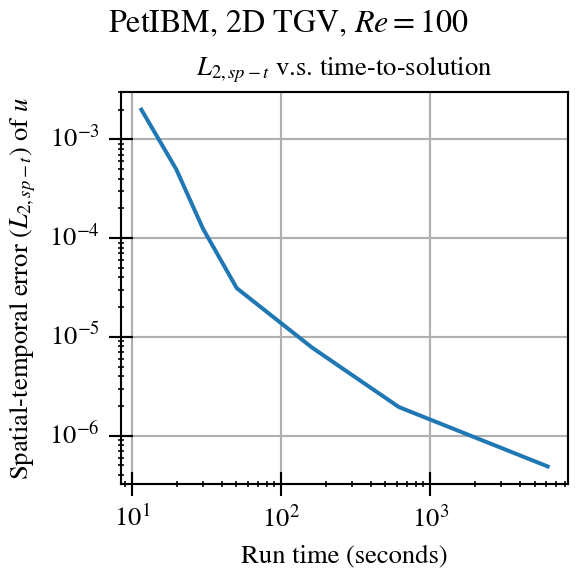
\includegraphics{tgv-2d-re100/petibm/tgv-2d-re100-err-u}%
    \caption[%
        PetIBM, TGV 2D $Re=100$: spatial-temporal error ($L_{2,sp-t}$) of $u$%
    ]{%
        PetIBM, TGV 2D $Re=100$: spatial-temporal error ($L_{2,sp-t}$)  of $u$ versus time-to-solution in seconds%
    }\label{fig:petibm-tgv-spatial-temporal-error}%
\end{figure}
We will be able to compare the time cost to get the desired error with conventional CFD code and with a PINN solver.
The configurations of PetIBM simulations can be found in section \ref{sec:petibm-vv}.
% vim:ft=tex


    \subsection{Result Visualizations}
    \label{sec:pinn-2d-tgv-vis}
    %! TEX root = main.tex

Before we use the cases in the first group for further benchmarking, we examine some results in this section.
We present the training histories and visualizations for the cases with the best, median, and worst $L_{2,sp-t}$ of $u$ velocity.
These cases correspond to $(N_l, N_n, N_{bs}) = (3, 256, 4096)$, $(2, 32, 65536)$, and $(1, 32, 16384)$, respectively.
And their $L_{2,sp-t}$ are $8.3e-3$, $1.4e-1$, and $3.1e-1$.
In the following discussion, we will use the format of $(N_l, N_n, N_{bs})$ to refer to the specific case we are discussing.

\begin{figure}[hbt!]
\centering%
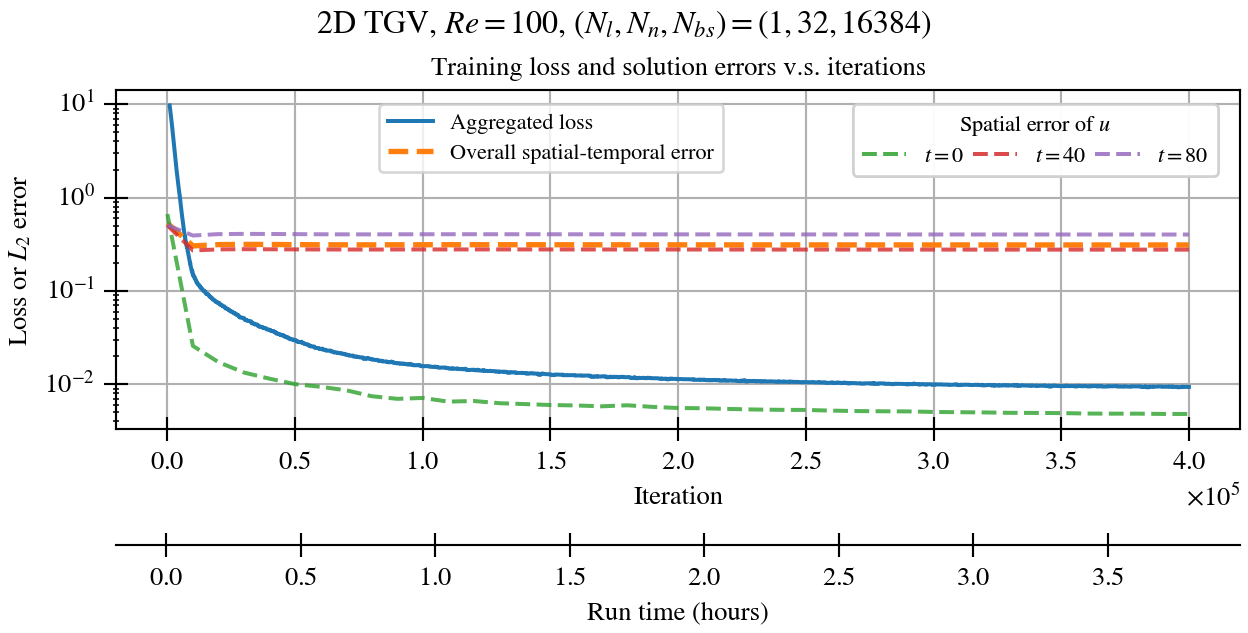
\includegraphics[width=0.9\linewidth]{tgv-2d-re100/training-hist/nl1-nn32-npts16384}%
\caption[%
    PINNs, 2D TGV, $Re=100$: Aggregated loss and $L_2$ errors of $u$ v.s. iterations ($(N_l, N_n, N_{bs})=(1, 32, 16384)$; the worst case)%
]{%
    PINNs, 2D TGV, $Re=100$: Aggregated loss and $L_2$ errors of $u$ v.s. iterations ($(N_l, N_n, N_{bs})$ $=$ $(1, 32, 16384)$; the worst case)%
}\label{fig:nl1-nn32-npts16384-loss-err-hist}%
\end{figure}

\begin{figure}[hbt!]
\centering%
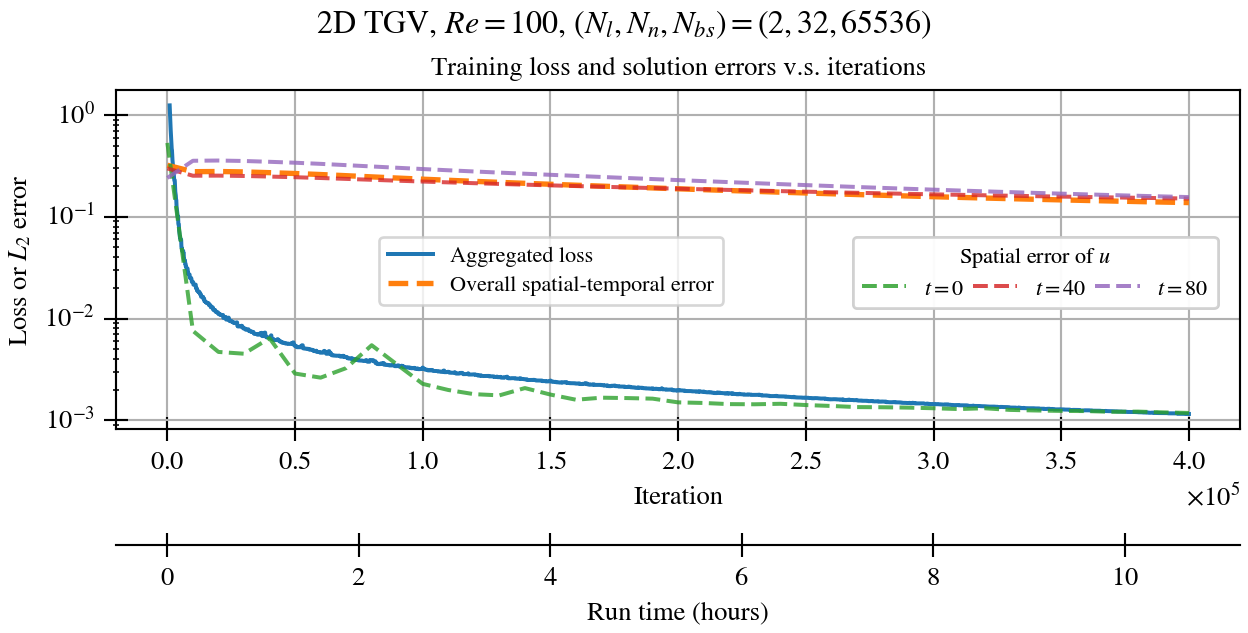
\includegraphics[width=0.9\linewidth]{tgv-2d-re100/training-hist/nl2-nn32-npts65536}%
\caption[%
    PINNs, 2D TGV, $Re=100$: Aggregated loss and $L_2$ errors of $u$ v.s. iterations ($(N_l, N_n, N_{bs})=(2, 32, 65536)$; the median case)%
]{%
    PINNs, 2D TGV, $Re=100$: Aggregated loss and $L_2$ errors of $u$ v.s. iterations ($(N_l, N_n, N_{bs})$ $=$ $(2, 32, 65536)$; the median case)%
}\label{fig:nl2-nn32-npts65536-loss-err-hist}%
\end{figure}

\begin{figure}[hbt!]
\centering%
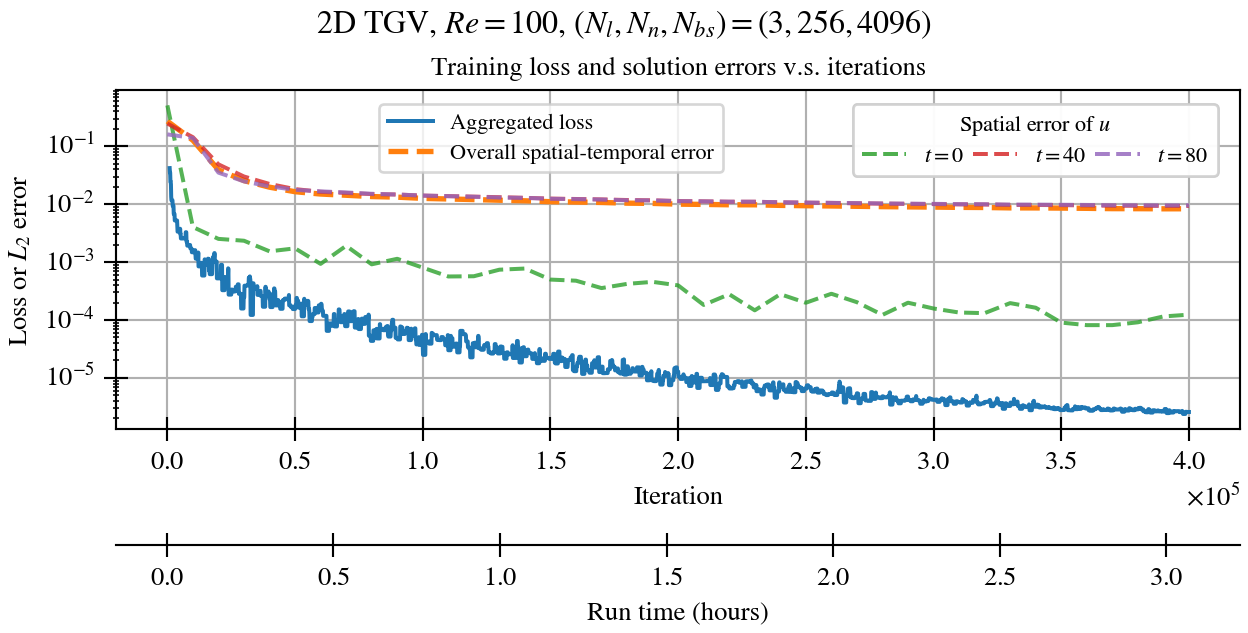
\includegraphics[width=0.9\linewidth]{tgv-2d-re100/training-hist/nl3-nn256-npts4096}%
\caption[%
    PINNs, 2D TGV, $Re=100$: Aggregated loss and $L_2$ errors of $u$ v.s. iterations ($(N_l, N_n, N_{bs})=(3, 256, 4096)$; the best case)%
]{%
    PINNs, 2D TGV, $Re=100$: Aggregated loss and $L_2$ errors of $u$ v.s. iterations ($(N_l, N_n, N_{bs})$ $=$ $(3, 256, 4096)$; the best case)%
}\label{fig:nl3-nn256-npts4096-loss-err-hist}%
\end{figure}

Figures \ref{fig:nl1-nn32-npts16384-loss-err-hist}, \ref{fig:nl2-nn32-npts65536-loss-err-hist}, and \ref{fig:nl3-nn256-npts4096-loss-err-hist} show how the aggregated loss $L_{2,sp-t}$, $L_2@t=0$, $L_2@t=40$, and $L_2@t=80$ for $u$ velocity progressed with training iterations.
A second $x$ axis at the bottom of these figures shows the corresponding run time (in hours).

Only the aggregated loss of $(1, 32, 16384)$ obviously converged, and the other two still show some potential to reach a smaller loss.
However, if we examine the history of $L_{2,sp-t}$, $L_2@t=40$, and $L_2@t=80$, the trends of these errors do not show much potential for improvement.
Especially from the case of $(3, 256, 4096)$, we see that the errors of $u$ does not change significantly after 200,000 iterations.
More training iterations only improve the error at $t=0$.
Note that the solution at $t=0$ is determined by the IC losses only, meaning the correct solution at $t=0$ is given to PINNs.
The solutions of $t=40$ and $t=80$ are mainly affected by PDE losses, and the PINNs do not have correct solutions.
The results shown in these figures mean that PINNs in this benchmark are only able to learn well from where we already provide explicit and correct answers.
PINNs do not perform well on solving the actual PDEs, where the solutions are unknown to them.
And learning well on IC does not help in solving the PDEs.

\begin{figure}[hbt!]
    \centering%
    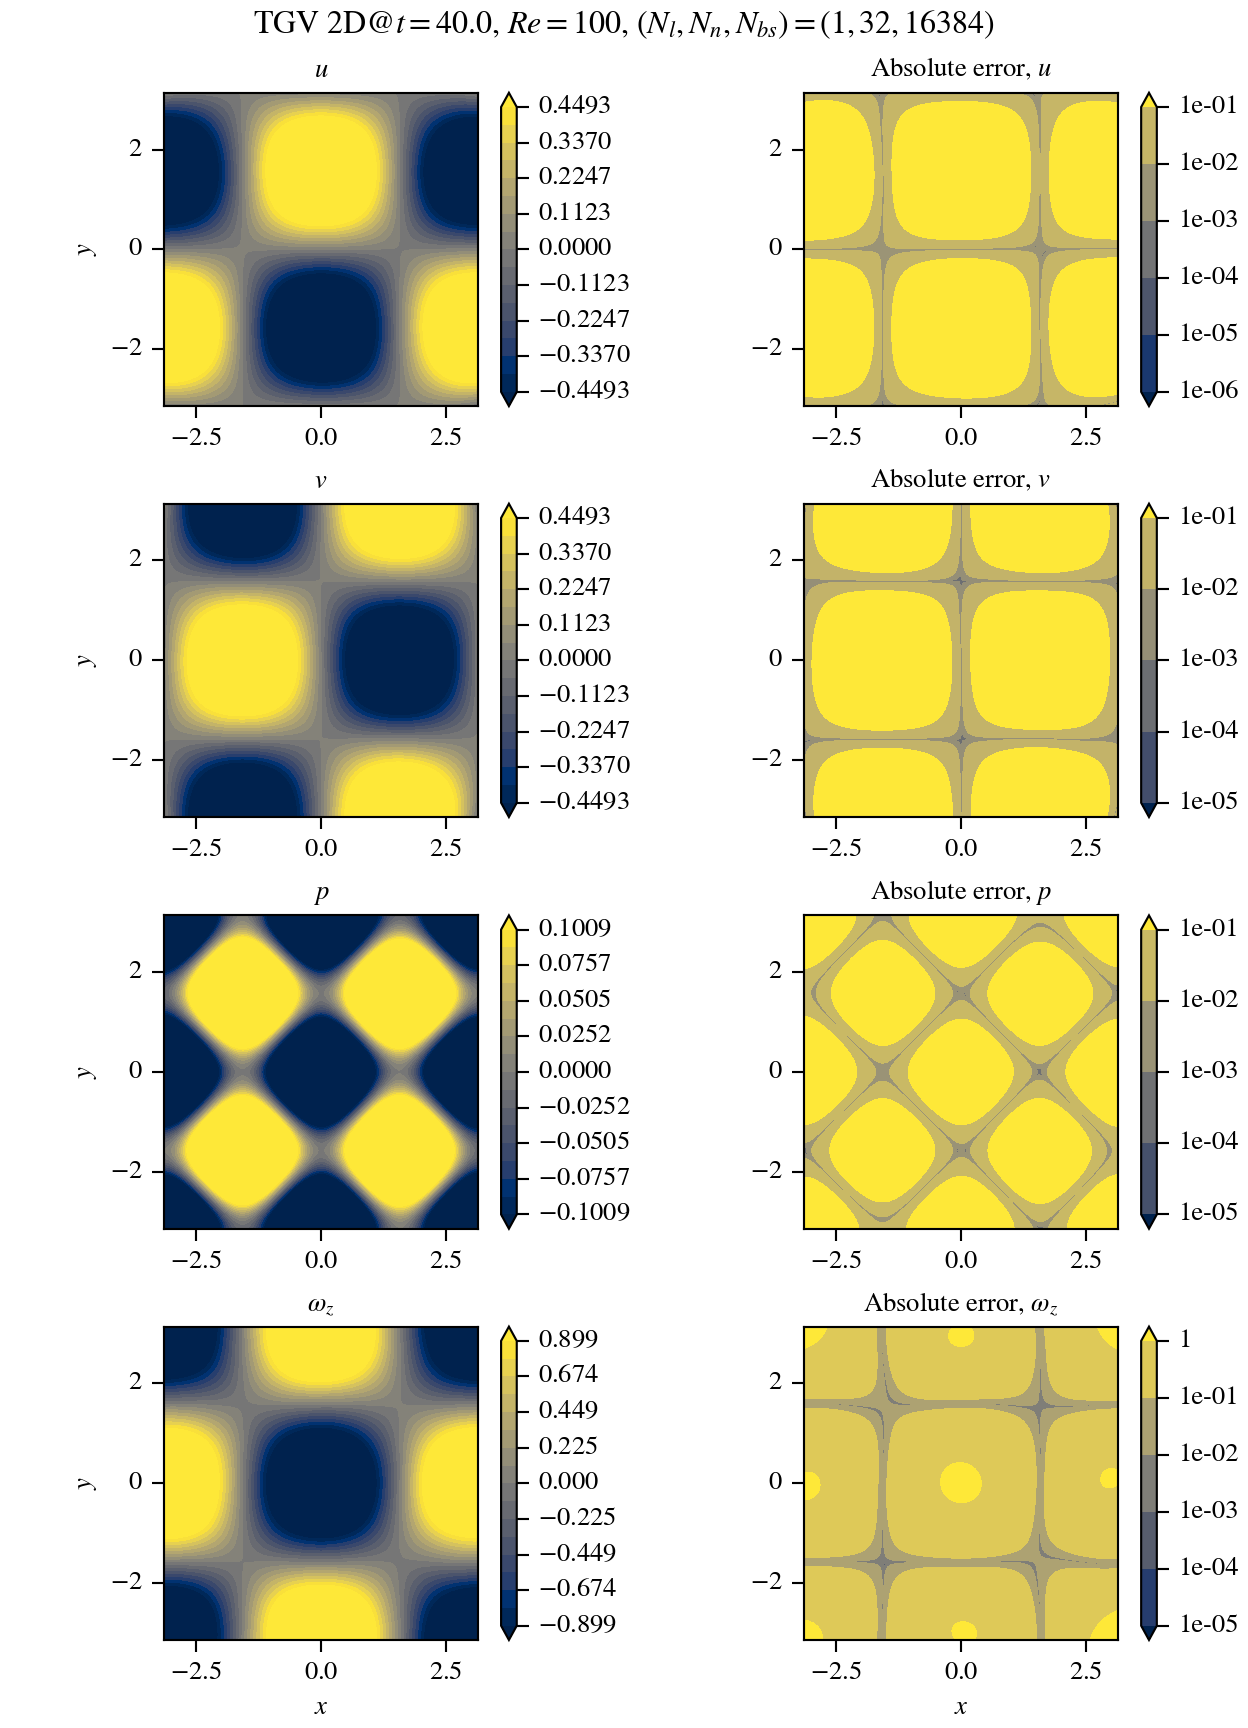
\includegraphics[width=0.9\linewidth]{tgv-2d-re100/contours/nl1-nn32-npts16384-t40.0.png}
    \caption[%
        PINNs, 2D TGV, $Re=100$: Predictions and error contours at $t=40$ ($(N_l, N_n, N_{bs})=(1, 32, 16384)$; the worst case)%
    ]{%
        PINNs, 2D TGV, $Re=100$: Predictions and error contours at $t=40$ ($(N_l, N_n, N_{bs})$ $=$ $(1, 32, 16384)$; the worst case)%
    }
    \label{fig:nl1-nn32-npts16384-t40-contours}
\end{figure}

\begin{figure}[hbt!]
    \centering%
    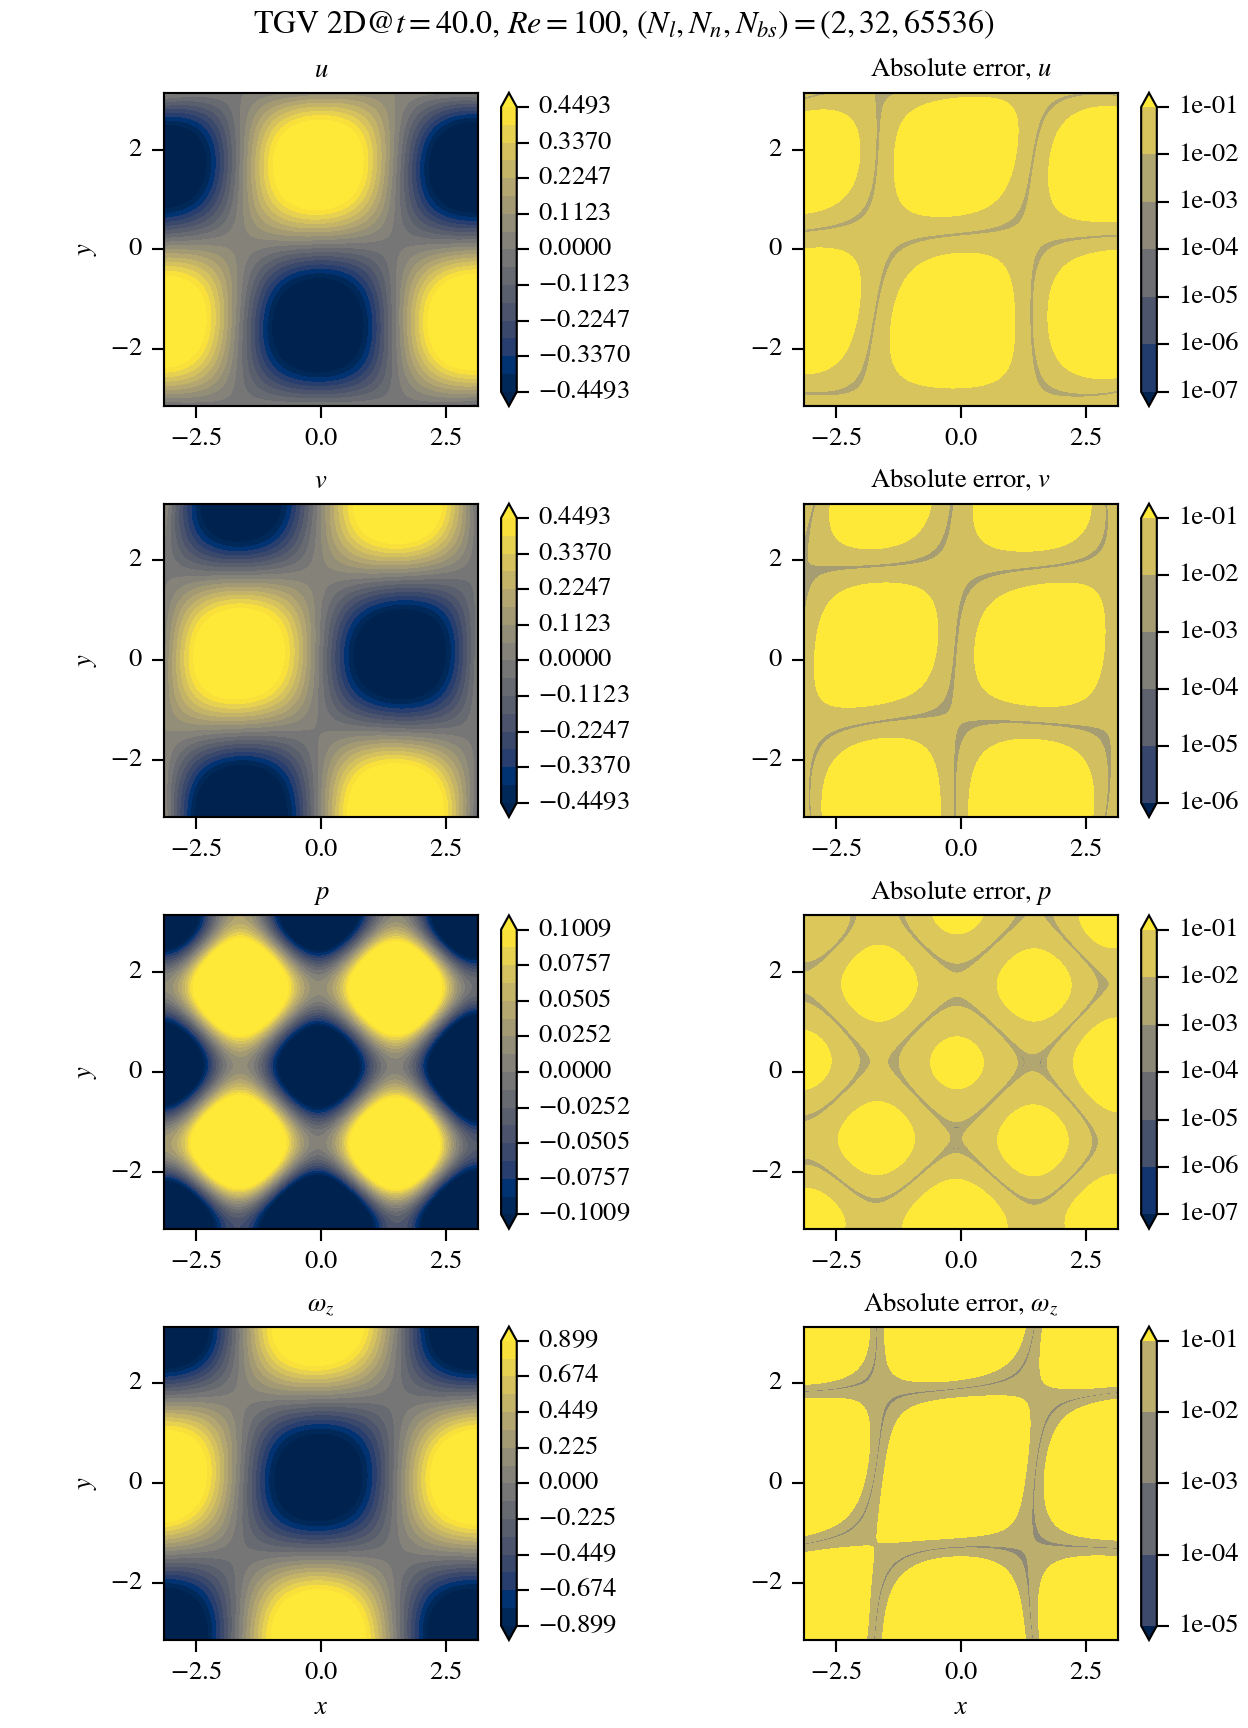
\includegraphics[width=0.9\linewidth]{tgv-2d-re100/contours/nl2-nn32-npts65536-t40.0}
    \caption[%
        PINNs, 2D TGV, $Re=100$: Predictions and error contours at $t=40$ ($(N_l, N_n, N_{bs})=(2, 32, 65536)$; the median case)%
    ]{%
        PINNs, 2D TGV, $Re=100$: Predictions and error contours at $t=40$ ($(N_l, N_n, N_{bs})$ $=$ $(2, 32, 65536)$; the median case)%
    }
    \label{fig:nl2-nn32-npts65536-t40-contours}
\end{figure}

\begin{figure}[hbt!]
    \centering%
    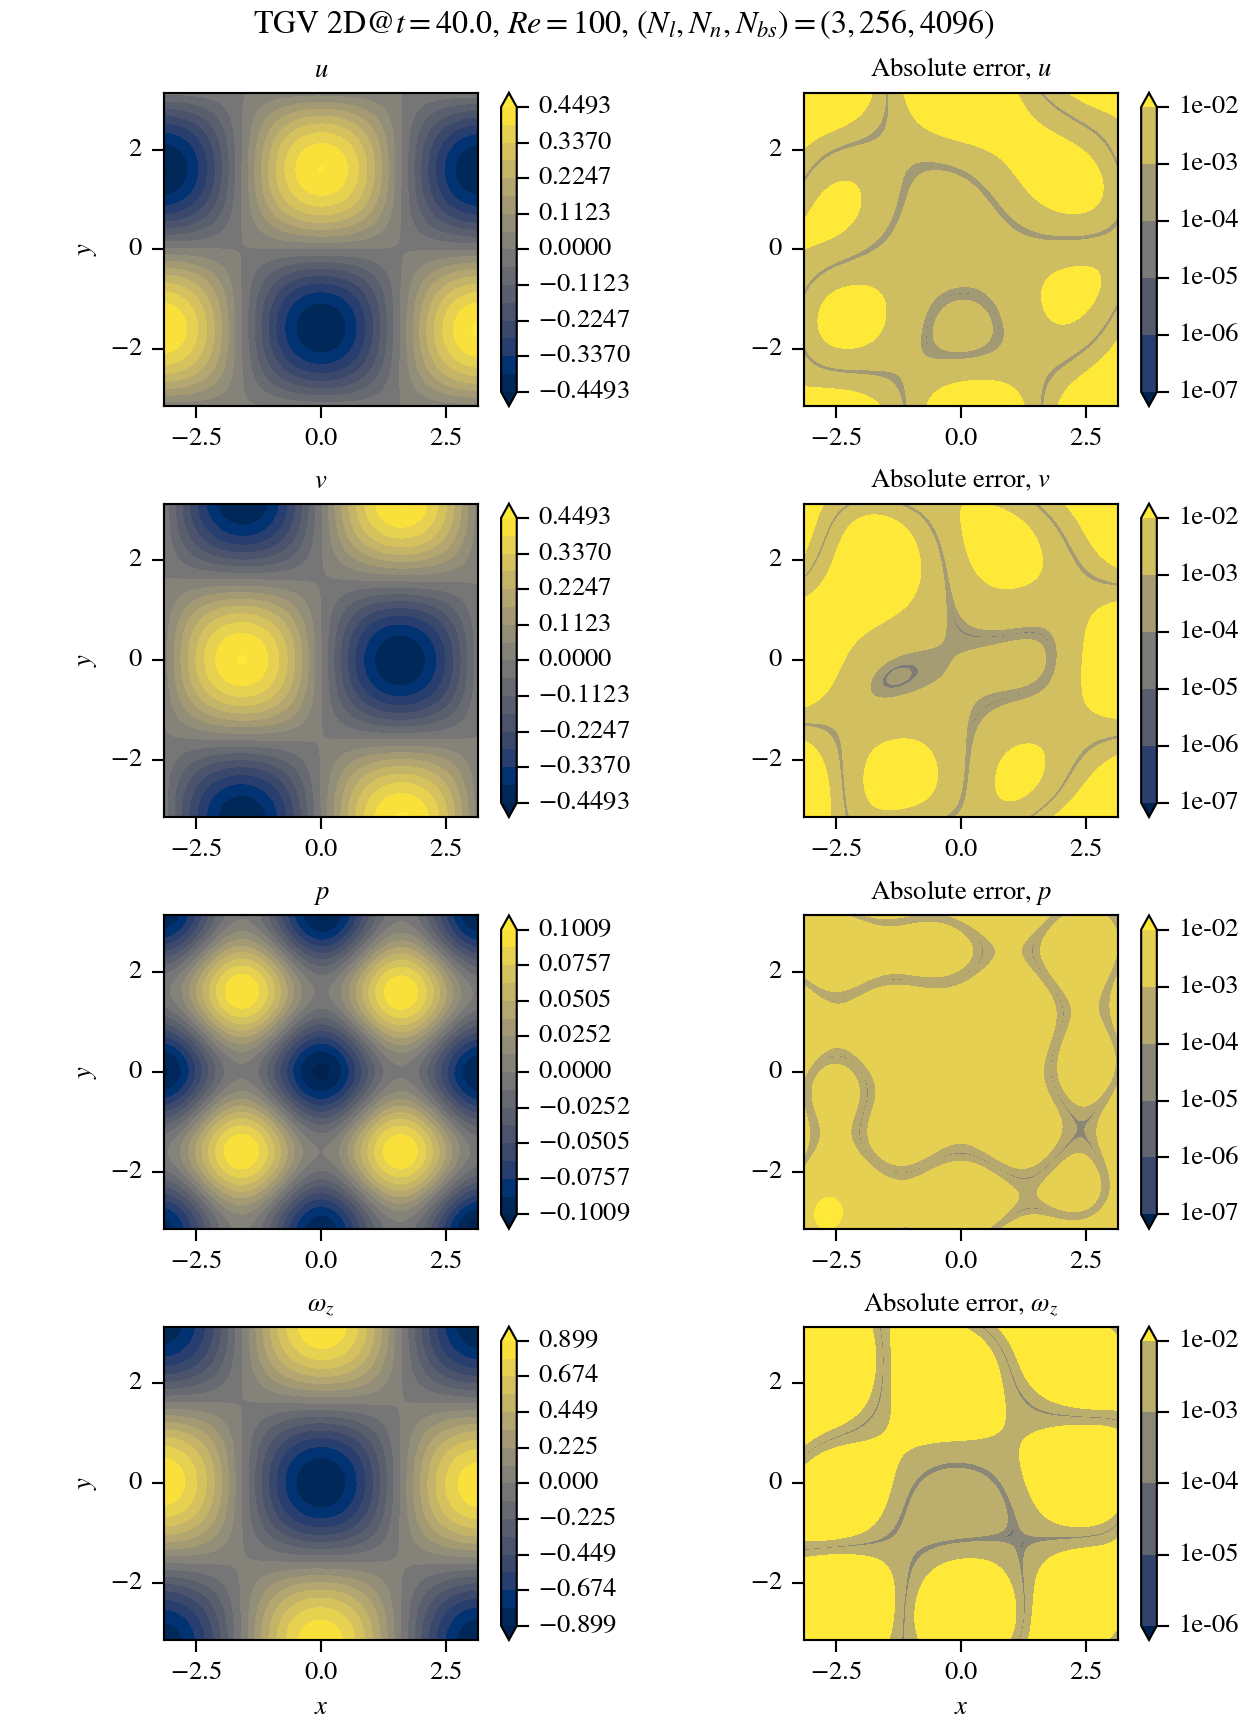
\includegraphics[width=0.9\linewidth]{tgv-2d-re100/contours/nl3-nn256-npts4096-t40.0.png}
    \caption[%
        PINNs, 2D TGV, $Re=100$: Predictions and error contours at $t=40$ ($(N_l, N_n, N_{bs})=(3, 256, 4096)$; the best case)%
    ]{%
        PINNs, 2D TGV, $Re=100$: Predictions and error contours at $t=40$ ($(N_l, N_n, N_{bs})$ $=$ $(3, 256, 4096)$; the best case)%
    }
    \label{fig:nl3-nn256-npts4096-t40-contours}
\end{figure}

If we compare the run times, the case of $(2, 32, 65536)$ took the longest, about 10.5 hours.
The case of $(1, 32, 16384)$ and $(3, 256, 4096)$ took about 3.8 and 3 hours, respectively.
Intuitively speaking, this observation shows that the run times are mainly dominated by the numbers of training points per batch rather than the complexity of a network.

We also compare the final $L_{2,sp-t}$ from the three cases with that in figure \ref{fig:petibm-tgv-spatial-temporal-error}.
While PetIBM was able to achieve an error level of $10^{-3}$ in less than 20 seconds, none of the three PINN cases was able to achieve the same level of error-cost ratio.

Figures \ref{fig:nl1-nn32-npts16384-t40-contours}, \ref{fig:nl2-nn32-npts65536-t40-contours}, and \ref{fig:nl3-nn256-npts4096-t40-contours} show the solution contours at $t=40$ for the three cases.
The color bars' levels are fixed according to the exact solution.
It is obvious that cases with $N_l=1$ and $N_l=2$ only work at where the exact solutions are zero.
The results are not even visually acceptable.
Only the case with $N_l=3$ is able to predict visually acceptable results.
It means both $(1, 16, 15384)$ and $(2, 32, 65536)$ underfit the solution, implying the model complexities are not enough in these two cases.
Later in section \ref{sec:pinn-2d-tgv-model-complexity}, we will see more comparison regarding the run times, model complexity, and the batch sizes.
% vim:ft=tex


    \subsection{Parallel Scalability}
    \label{sec:pinn-2d-tgv-scaling}
    %! TEX root = main.tex

In this section, we are interested in the scalability of PINNs.
In the weak scaling tests, we scaled $(2, 32, 8192)$ and $(3, 128, 8192)$ with 1, 2, 4, and 8 GPUs. 
As for the strong scaling tests, we scaled $(2, 32, 65536)$ and $(3, 128, 65536)$ with 1, 2, 4, and 8 GPUs. 
We will use an expression of $(N_l, N_n, N_{bs})\times N_{gpu}$ to denote how many GPUs are used and how many training points per batch on each GPU.
On the other, an expression of $(N_l, N_n, N_{bs}\times N_{gpu})$ denotes a case running on only one GPU but has $N_{bs}\times N_{gpu}$ training points per batch.

Figures \ref{fig:nl2-nn32-npts8192-weak-scaling} and \ref{fig:nl3-nn128-npts8192-weak-scaling} show the results of weak scaling tests.
These figures show the losses and errors of $u$ versus iterations on the left $y$-axis.
And for the other $y$-axis, we have the run times in hours versus iterations.

\begin{figure}[hbt!]
    \centering%
    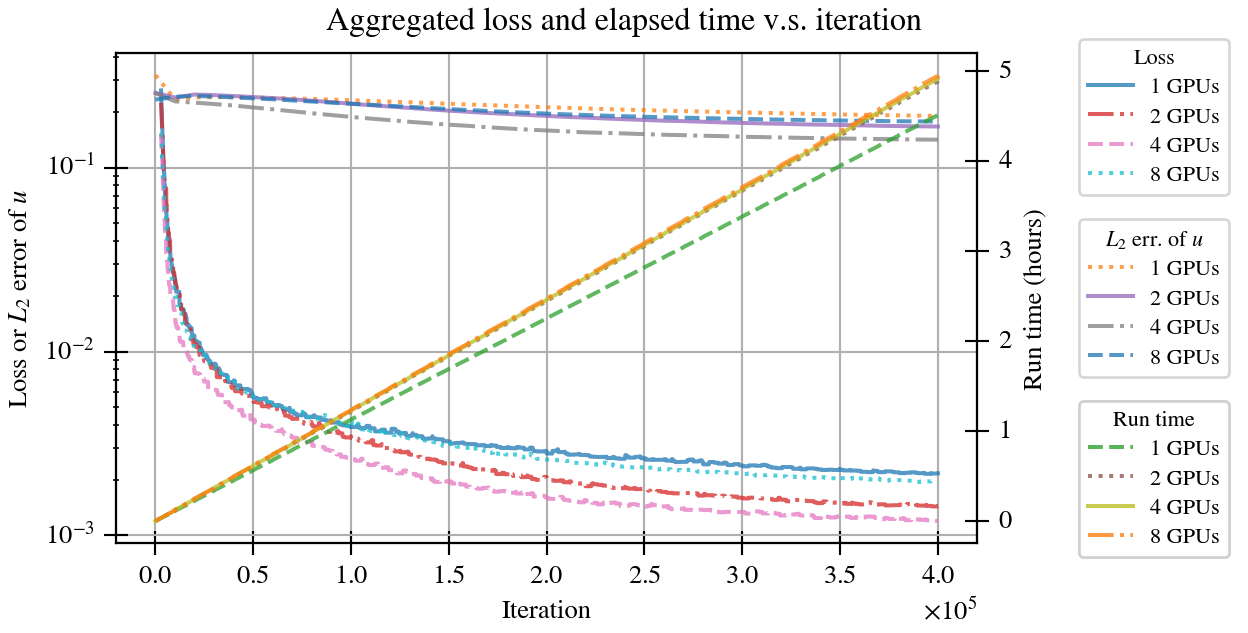
\includegraphics[width=0.9\linewidth]{tgv-2d-re100/scaling-tests/nl2-nn32-npts8192-weak-scaling.png}
    \caption[%
        Weak scaling: aggregated loss and run time v.s. iteration ($(N_l, N_n, N_{bs})$ $=$ $(2, 32, 8192)$)%
    ]{%
        Weak scaling: aggregated loss and run time v.s. iteration ($(N_l, N_n, N_{bs})$ $=$ $(2, 32, 8192)$)%
    }\label{fig:nl2-nn32-npts8192-weak-scaling}
\end{figure}

\begin{figure}[hbt!]
    \centering%
    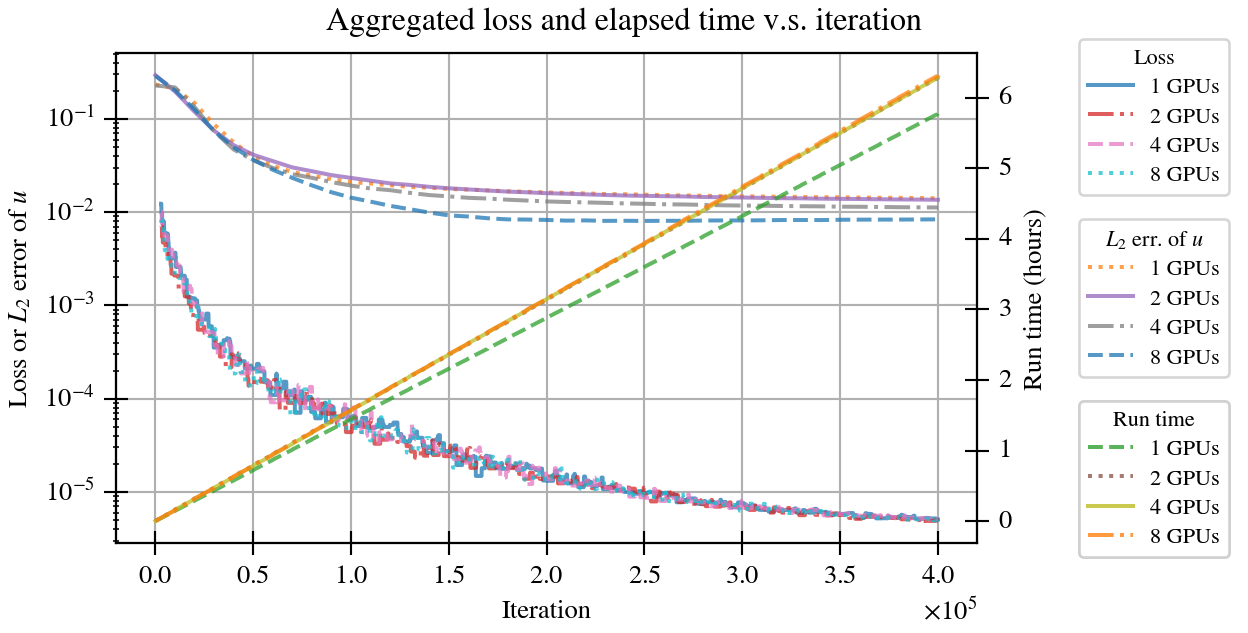
\includegraphics[width=0.9\linewidth]{tgv-2d-re100/scaling-tests/nl3-nn128-npts8192-weak-scaling.png}
    \caption[%
        Weak scaling: aggregated loss and run time v.s. iteration ($(N_l, N_n, N_{bs})$ $=$ $(3, 128, 8192)$)%
    ]{%
        Weak scaling: aggregated loss and run time v.s. iteration ($(N_l, N_n, N_{bs})$ $=$ $(3, 128, 8192)$)%
    }\label{fig:nl3-nn128-npts8192-weak-scaling}
\end{figure}

In weak scaling, because each GPU has the same amount of work loading, the run time versus iterations should be the same for different cases.
From figure \ref{fig:nl2-nn32-npts8192-weak-scaling} and \ref{fig:nl3-nn128-npts8192-weak-scaling}, we found that, except for the 1-GPU cases, cases with other GPUs match each other.
The reason that 1-GPU cases show different results may be that it does not have the latency overhead due to exchanging with other GPUs.

We further checked the losses and error histories and considered no significant difference between using different numbers of GPUs.
Note that while lines do not overlap on the figures, quantitatively speaking, the difference in the orders of magnitude is minor, as we will see in table \ref{table:weak-scaling-perf}. 

Theoretically, $(N_l, N_n, N_{bs})\times N_{gpu}$ is expected to equal to $(N_l, N_n, N_{bs}\times N_{gpu})$ in terms of losses and errors.
So the difference between using a different number of GPUs should be similar to the effect of using a different number of training points per batch on one GPU.
We will examine the effect of different $N_{bs}$ in section \ref{sec:pinn-2d-tgv-model-complexity}.
Instead, here we would like to check if it is true that $(N_l, N_n, N_{bs})\times N_{gpu}$ is equivalent to $(N_l, N_n, N_{bs}\times N_{gpu})$.
Figure \ref{fig:nl2-nn32-npts8192-multi-singl-gpus} shows the comparisons between $(2, 32, 8192)\times N_{gpu}$ and $(2, 32, 8192\times N_{gpu})$.
And figure \ref{fig:nl3-nn128-npts8192-multi-singl-gpus} shows the same comparisons between $(3, 128, 8192)\times N_{gpu}$ and $(3, 128, 8192\times N_{gpu})$.

\begin{figure}[hbt!]
    \centering%
    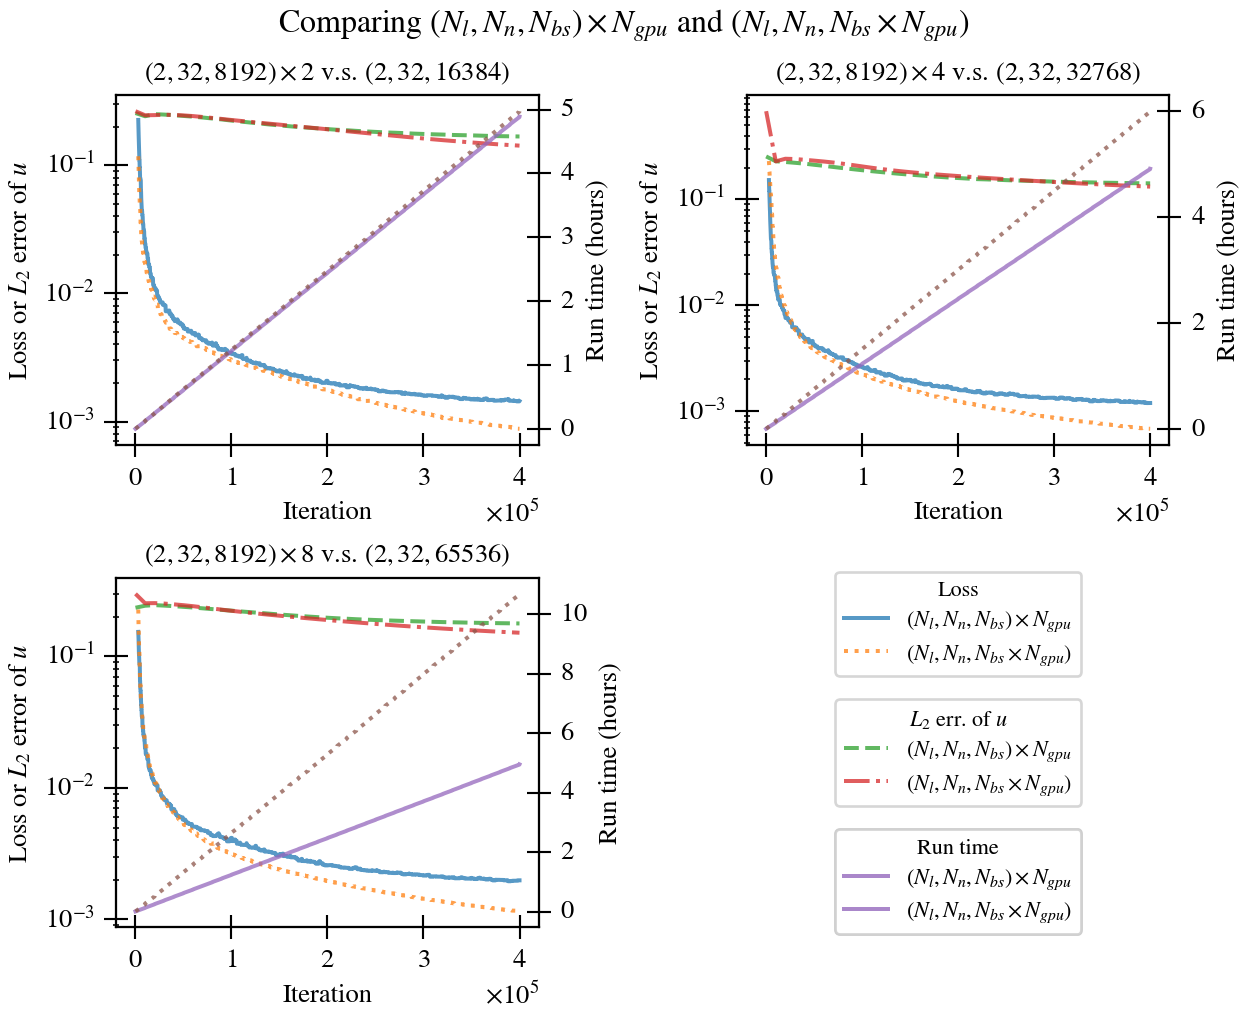
\includegraphics[width=0.9\linewidth]{tgv-2d-re100/scaling-tests/nl2-nn32-npts8192-multi-singl-gpus.png}
    \caption[%
        Comparing multi-GPU and single-GPU cases ($(N_l, N_n)$ $=$ $(2, 32)$)%
    ]{%
        Comparing multi-GPU and single-GPU cases ($(N_l, N_n)$ $=$ $(2, 32)$)%
    }\label{fig:nl2-nn32-npts8192-multi-singl-gpus}
\end{figure}

\begin{figure}[hbt!]
    \centering%
    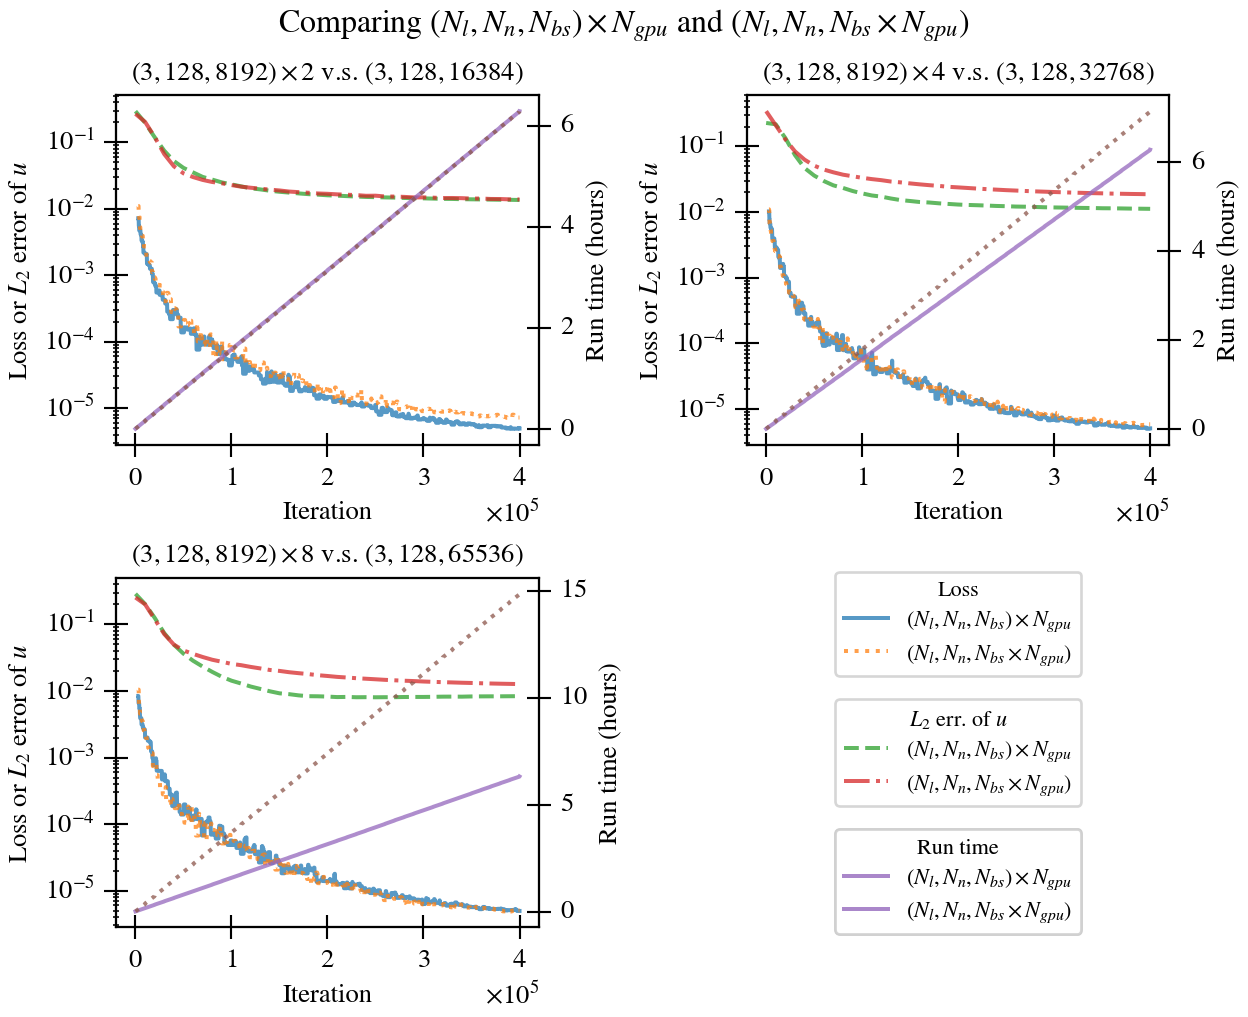
\includegraphics[width=0.9\linewidth]{tgv-2d-re100/scaling-tests/nl3-nn128-npts8192-multi-singl-gpus.png}
    \caption[%
        Comparing multi-GPU and single-GPU cases ($(N_l, N_n)$ $=$ $(3, 128)$)%
    ]{%
        Comparing multi-GPU and single-GPU cases ($(N_l, N_n)$ $=$ $(3, 128)$)%
    }\label{fig:nl3-nn128-npts8192-multi-singl-gpus}
\end{figure}

In these figures, it is expected that the run times are different and that the losses and errors are similar.
However, though losses and errors show similar trends between $(N_l, N_n, N_{bs})\times N_{gpu}$ and $(N_l, N_n, N_{bs}\times N_{gpu})$, visible differences exist.
In $(N_l, N_n)=(2, 32)$, losses stop improving earlier for multi-GPU cases, and multi-GPU cases have slightly worse errors.
On the other hand, for $(N_l, N_n)=(3, 128)$, the multi-GPU cases in general have better errors, though the loss histories do not show a noticeable difference.
The reason is unknown to us at this point.
The observation shows that $(N_l, N_n, N_{bs})\times N_{gpu}$ and $(N_l, N_n, N_{bs}\times N_{gpu})$ are not necessarily the same.
Nevertheless, we believe the differences are quantitatively minor if we consider their orders of magnitude.

\begin{table}[hbt!]
\centering
\singlespacing
\caption[
    PINNs, 2D TGV, $Re=100$: weak scaling performance for $(N_l, N_n, N_{bs})=(2, 32, 8192)$ and $(3, 128, 8192)$
]{
    Weak scaling performance for $(N_l, N_n, N_{bs})$ $=$ $(2, 32, 8192)$ and $(3, 128, 8192)$.%
    Time costs denote the wall time required to finish 400k training iterations in hours.%
    Efficiency here stands for weak scaling efficiency in $\%$.%
    The aggregated losses are those at the last iteration.%
    The $L_{2, sp-t}$ errors were the overall spatial-temporal errors at the last training iteration.%
}
\label{table:weak-scaling-perf}
\begin{tabular}{lcccccccc}
\toprule
 & \multicolumn{4}{c}{(2, 32, 8192)} & \multicolumn{4}{c}{(3, 128, 8192)} \\
\cmidrule(rl){2-5} \cmidrule(rl){6-9}
\multicolumn{1}{r}{GPUs} & 1 & 2 & 4 & 8 & 1 & 2 & 4 & 8 \\
\midrule
Time cost &  4.51 &  4.89 &  4.92 &  4.95 &  5.77 &  6.28 &  6.29 &  6.32 \\
\addlinespace
Efficiency & 100 & 92 & 92 & 91 & 100 & 92 & 92 & 91 \\
\addlinespace
Loss & 2.2e-03 & 1.5e-03 & 1.2e-03 & 2.1e-03 & 6.7e-06 & 5.3e-06 & 5.5e-06 & 5.3e-06 \\
\addlinespace
$L_{2,sp-t}$, $u$ & 1.9e-01 & 1.5e-01 & 1.2e-01 & 1.7e-01 & 1.3e-02 & 1.3e-02 & 1.0e-02 & 8.9e-03 \\
\addlinespace
$L_{2,sp-t}$, $v$ & 1.9e-01 & 1.5e-01 & 1.3e-01 & 1.8e-01 & 1.1e-02 & 1.2e-02 & 1.1e-02 & 9.6e-03 \\
\bottomrule
\end{tabular}
\end{table}


The quantitative results are listed in table \ref{table:weak-scaling-perf}.
The weak-scaling efficiencies are all above $90\%$.
The losses and errors are close in terms of the orders of magnitude.
PINNs generally have good weak-scaling if we define the workload using $N_{bs}$.
During training, each GPU calculates the gradients $\nabla_{\Theta} r(\Theta)$ independently, and then each training iteration only needs one reduction operation to calculate the averaged gradients across all GPUs.
A good weak scaling is thus expected.

Lastly, we examined the strong scaling.
Figure \ref{fig:nl2-nn32-npts65536-strong-scaling} shows the strong scaling results of $(2, 32, 65535)\times 1$, $(2, 32, 32768)\times 2$, $(2, 32, 16384)\times 4$, and $(2, 32, 8192)\times 8$.
Figure \ref{fig:nl3-nn128-npts65536-strong-scaling} shows the similar strong scaling tests for $(N_l, N_n)=(3, 128)$.
Quantitative results are listed in table \ref{table:strong-scaling-perf}. 

\begin{figure}[hbt!]
    \centering%
    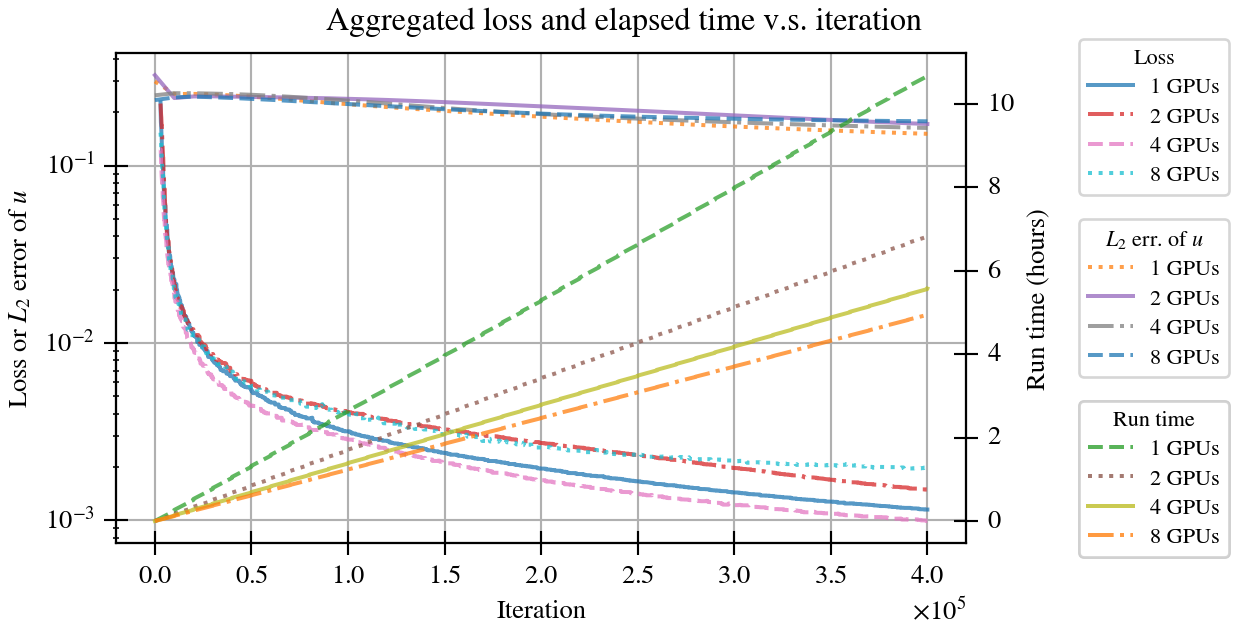
\includegraphics[width=0.9\linewidth]{tgv-2d-re100/scaling-tests/nl2-nn32-npts65536-strong-scaling.png}
    \caption[%
        Strong-scaling: aggregated loss and run time v.s. iteration ($(N_l, N_n, N_{bs})$ $=$ $(2, 32, 65535)$)%
    ]{%
        Strong-scaling: aggregated loss and run time v.s. iteration ($(N_l, N_n, N_{bs})$ $=$ $(2, 32, 65535)$)%
    }\label{fig:nl2-nn32-npts65536-strong-scaling}
\end{figure}

\begin{figure}[hbt!]
    \centering%
    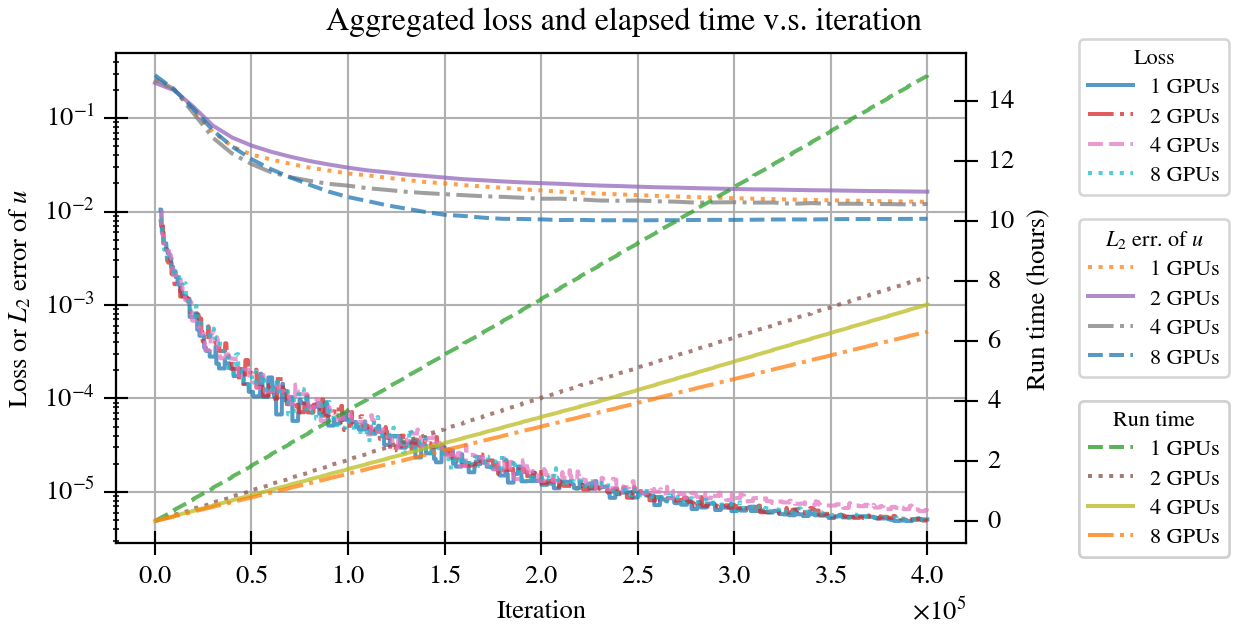
\includegraphics[width=0.9\linewidth]{tgv-2d-re100/scaling-tests/nl3-nn128-npts65536-strong-scaling.png}
    \caption[%
        Strong-scaling: aggregated loss and run time v.s. iteration ($(N_l, N_n, N_{bs})$ $=$ $(3, 128, 65535)$)%
    ]{%
        Strong-scaling: aggregated loss and run time v.s. iteration ($(N_l, N_n, N_{bs})$ $=$ $(3, 128, 65535)$)%
    }\label{fig:nl3-nn128-npts65536-strong-scaling}
\end{figure}

Theoretically, a good strong scaling result should show similar losses and errors.
Figures \ref{fig:nl2-nn32-npts65536-strong-scaling} and \ref{fig:nl3-nn128-npts65536-strong-scaling}, instead, exhibit some differences.
However, if we consider their orders of magnitude, we consider the differences minor.
This claim can be examined from table \ref{table:strong-scaling-perf}.
On the other hand, the results show deteriorating strong scaling efficiencies.
The worse strong scaling is caused by only dividing the training points across GPUs, while the model itself is not divided.  
The model complexity also contributes to the work loading.
We do not have a clear way to divide a model and distribute the work loading across GPUs.
Neither do we have means to exclude the model's contribution to the work loading and correctly calculate the strong scaling efficiencies and speedups.
Lacking these knowledges limited our investigation into the strong scaling of PINNs.

\begin{table}[hbt!]
\centering
\singlespacing
\caption[
    PINNs, 2D TGV, $Re=100$: strong scaling performance for $(N_l$, $N_n$, $N_{bs})$ $=$ $(2$, $32$, $65536)$ and $(3$, $128$, $65536)$
]{
    Strong scaling performance for $(N_l$, $N_n$, $N_{bs})$ $=$ $(2$, $32$, $65536)$ and $(3$, $128$, $65536)$.%
    Time costs denote the wall time required to finish 400k training iterations in hours.%
    Efficiency here stands for strong scaling efficiency in $\%$.%
    The aggregated losses were those at the last iteration.%
    The $L_{2,sp-t}$ errors were the overall spatial-temporal errors at the last training iteration.%
}
\label{table:strong-scaling-perf}
\begin{tabular}{lcccccccc}
\toprule
 & \multicolumn{4}{c}{(2, 32, 65536)} & \multicolumn{4}{c}{(3, 128, 65536)} \\
\cmidrule(rl){2-5} \cmidrule(rl){6-9}
\multicolumn{1}{r}{GPUs} & 1 & 2 & 4 & 8 & 1 & 2 & 4 & 8 \\
\midrule
Time cost & 10.69 &  6.82 &  5.57 &  4.95 & 14.79 &  8.12 &  7.23 &  6.32 \\
\addlinespace
Speedup & 1.0x & 1.6x & 1.9x & 2.2x & 1.0x & 1.8x & 2.0x & 2.3x \\
\addlinespace
Efficiency & 100 & 78 & 48 & 27 & 100 & 91 & 51 & 29 \\
\addlinespace
Loss & 1.2e-03 & 1.5e-03 & 1.0e-03 & 2.1e-03 & 5.1e-06 & 5.2e-06 & 6.7e-06 & 5.3e-06 \\
\addlinespace
$L_{2,sp-t}$, $u$ & 1.4e-01 & 1.6e-01 & 1.5e-01 & 1.7e-01 & 1.1e-02 & 1.6e-02 & 1.2e-02 & 8.9e-03 \\
\addlinespace
$L_{2,sp-t}$, $v$ & 1.4e-01 & 1.6e-01 & 1.5e-01 & 1.8e-01 & 1.0e-02 & 1.7e-02 & 1.2e-02 & 9.6e-03 \\
\bottomrule
\end{tabular}
\end{table}

% vim:ft=tex

    \subsection{Aggregate Loss and Prediction Accuracy}
    \label{sec:pinn-2d-tgv-loss-vs-accuracy}
    %! TEX root = main.tex
One particular question we would like to investigate is the relationship between training loss and the actual prediction errors or accuracy.
As we have seen from the previous section, further training in many cases only reduces the IC losses, while the PDE losses already converged.
Reductions in IC losses, though they improve the prediction error of the solution at $t=0$, do not help the overall spatial-temporal $L_{2,sp-t}$ at all.
This implies the training loss may not reflect the models' prediction capabilities.
If true, then the aggregated loss is not a sufficient indicator to monitor the training progress.
Also, given a known aggregated loss and error, we may not able to predict how much loss we need to further reduce and achieve a desired error level.
We would hence like to investigate the relationship between the aggregated loss and the overall spatial-temporal errors.

Figure \ref{fig:tgv2d-re100-err-vs-loss} shows the $L_{2,sp-t}$ of all cases.
The $x$-axis represents the square roots of aggregate losses, and the $y$-axis is $L_{2,sp-t}$ of $u$ and $v$.
For each case, $u$ and $v$ are separate dots in the figure.
The figure uses the square roots of aggregate losses because losses are defined as the sum of residuals' squares.
See equation \eqref{eq:residual-norms}

\begin{figure}[hbt!]
    \centering%
    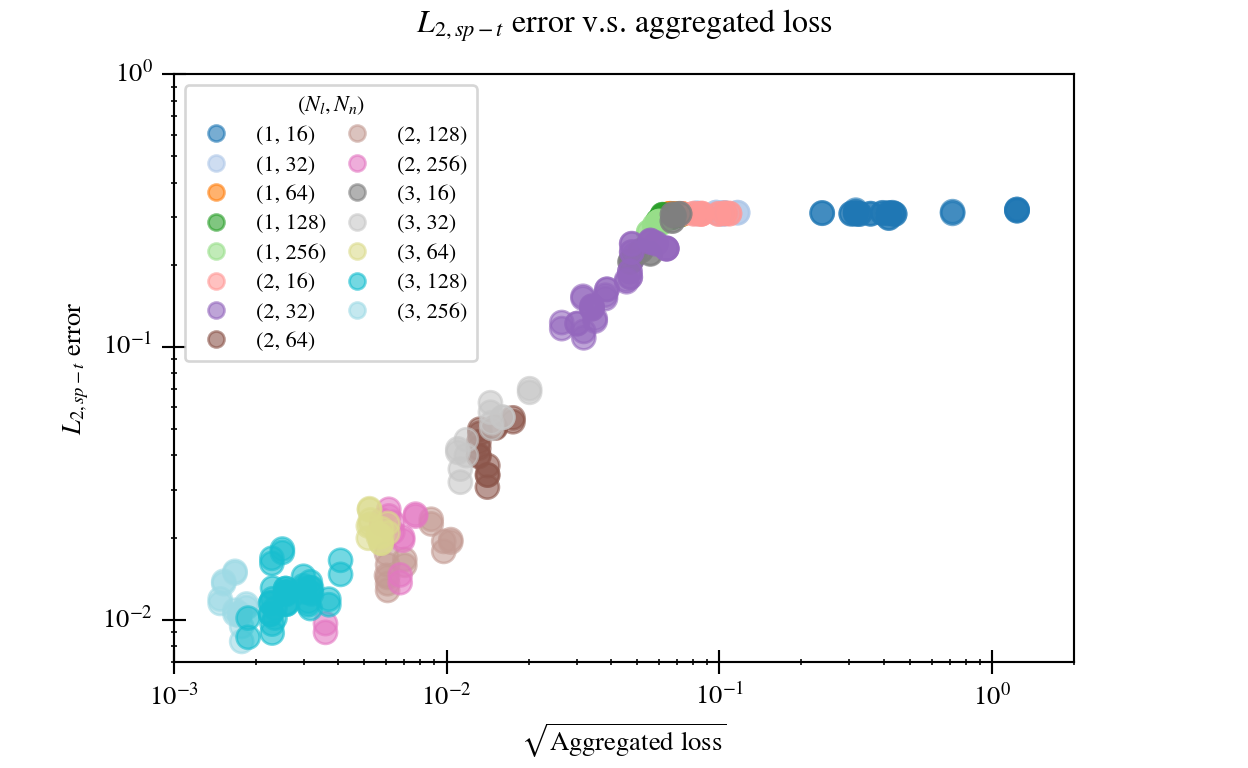
\includegraphics[width=0.9\linewidth]{tgv-2d-re100/err-vs-loss/err-loss.png}
    \caption[%
        PINNs, 2D TGV, $Re=100$: $L_{2,sp-t}$ error v.s. aggregated loss%
    ]{%
        PINNs, 2D TGV, $Re=100$: $L_{2,sp-t}$ error v.s. aggregated loss. %
        $L_{2,sp-t}$ errors for $u$ and $v$ from the same case are separate data points in the figure.
    }
    \label{fig:tgv2d-re100-err-vs-loss}
\end{figure}

From the figure, the first observation is the flat region in the top-right corner.
These cases are mainly those with only one hidden layer, implying that one hidden layer may not be enough to approximate the solutions of the Navier-Stokes equations.

Although the relationship is approximately linear in the middle range, the data points become more scattered in the bottom-left corner, and a similar loss level has a wider range of possible $L_{2,sp-t}$.
Given the observed trends, it is reasonable to suspect that, if we had more data further to the left of this figure, the possible $L_{2,sp-t}$ corresponding to a loss level may have a wider and wider scatter, meaning it is more difficult to predict the solution accuracy for a given training loss.

In addition, we suspect that using adaptive loss weighting like annealing loss aggregation may exacerbate the problem.
As each loss term's weight is updated according to the ratio of characteristic gradient magnitudes, it is likely that two iterations will have the same level of aggregated losses but have different prediction accuracies. 
This observation somehow hurts the predictability of PINNs.
Especially when dealing with real-world problems where we don't have exact solutions to calculate the errors, the losses may be the only indicator for us to estimate a model's prediction capability.
If lowering the loss does not improve the prediction accuracy, we have no means to know if training should keep going.
% vim:ft=tex


    \subsection{Model Complexity, Batch Sizes, and Time Costs}
    \label{sec:pinn-2d-tgv-model-complexity}
    %! TEX root = main.tex

In conventional numerical methods, the degrees of freedom (i.e., the numbers of model parameters) reflect the model complexity.
And given a numerical method and a model complexity, the workload, time cost, and accuracy are theoretically predictable.
In PINNs, the number of model parameters also determines the model complexity.
However, even with a specific PINN implementation, model complexity may not be the only factor determining the time cost and the accuracy.
The number of training points per batch ($N_{bs}$) apparently also influences the time cost.
One interesting question is whether $N_{bs}$ affects the prediction accuracy or errors.
If yes, then how to choose a proper $N_{bs}$ is a follow-up question. 
If no, it means the time cost does not reflect the PINN methods' performance.
In this section, we would like to examine the relationship between model complexity, batch sizes, error levels, and the time costs.

We first visualize the $L_{2,sp-t}$ errors of $u$ for all cases in figure \ref{fig:tgv2d-re100-err-vs-arch}.
\begin{figure}[hbt!]
    \centering%
    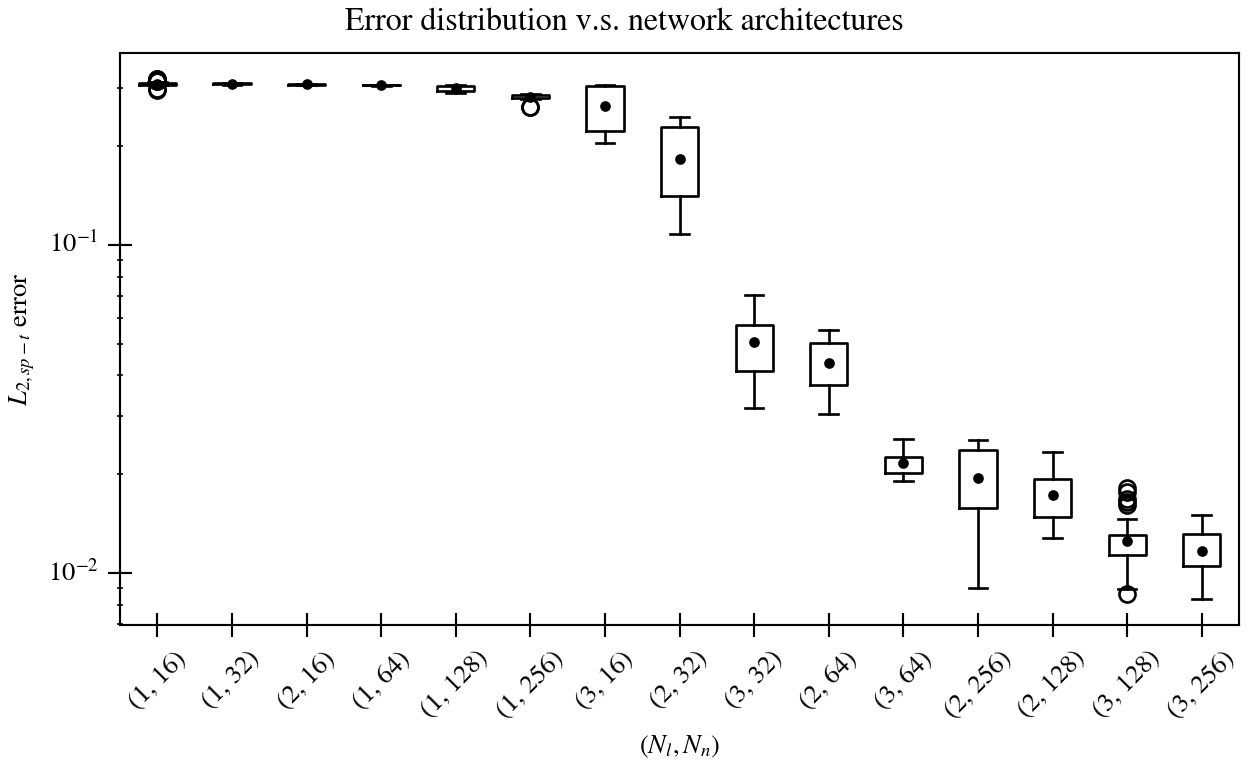
\includegraphics[width=0.95\linewidth]{tgv-2d-re100/err-vs-model-complexity/err-arch-boxplot}
    \caption[%
        PINNs, 2D TGV, $Re=100$: $L_{2,sp-t}$ error v.s. network architecture%
    ]{%
        PINNs, 2D TGV, $Re=100$: $L_{2,sp-t}$ error v.s. network architecture%
    }
    \label{fig:tgv2d-re100-err-vs-arch}
\end{figure}
The $y$-axis is $L_{2,sp-t}$, and $x$-axis denotes the network architectures $(N_l, N_n)$.
The architectures are sorted by their error magnitudes from left to right.
The box plot of each architecture represents the error distributions of different $N_{bs}$ with the same architecture.
We hope this figure can shed some light on how $N_l$, $N_n$, and $N_{bs}$ influence the error levels.
The figure shows that, when $N_l < 2$ or $N_n < 32$, the errors remain at the same level, and $N_{bs}$ does not have any influence.
This may indicate these models are too simple and always underfit the PDEs.
Once the model complexity reaches a certain level, increasing both $N_n$ and $N_l$ helps lower the error levels.
Also, $N_{bs}$ starts to have an effect in these cases.
Nevertheless, if we consider the orders of magnitudes, quantitatively speaking, we don't consider that $N_{bs}$ has a strong impact on the accuracy.
As seen from the figure, model complexity still dominates the error levels. 

It is unclear from figure \ref{fig:tgv2d-re100-err-vs-arch} whether increasing $N_l$ or $N_n$ has a stronger impact on the error levels.
For example, if we are to improve the error level of $(N_l$, $N_n)$ $=$ $(2$, $32)$, both $(2$, $64)$ and $(3$, $32)$ give us similar improvement.
Or, if we are to improve the error of $(2$, $64)$, both $(2$, $128)$ and $(3$, $64)$ give a similar level of errors.
Though increasing $N_l$ or doubling $N_n$ have the same effect in terms of the error levels, their effects in the total number of model parameters are different. 
As seen from equation \eqref{eq:dof-calculator}, the degrees of freedom increase about linearly with $N_l$ but increase proportionally to the square of $N_n$.
In other words, doubling $N_n$ roughly quadruples the number of free parameters, while increasing $N_l$ by one just adds around $N_n^2$ parameters.
Hence, form the viewpoint of computational cost, increasing $N_l$ may be a better choice.

Figure \ref{fig:tgv2d-re100-err-vs-dof} shows a similar box plots but with the $x$-axis being the degrees of freedom.
\begin{figure}[hbt!]
    \centering%
    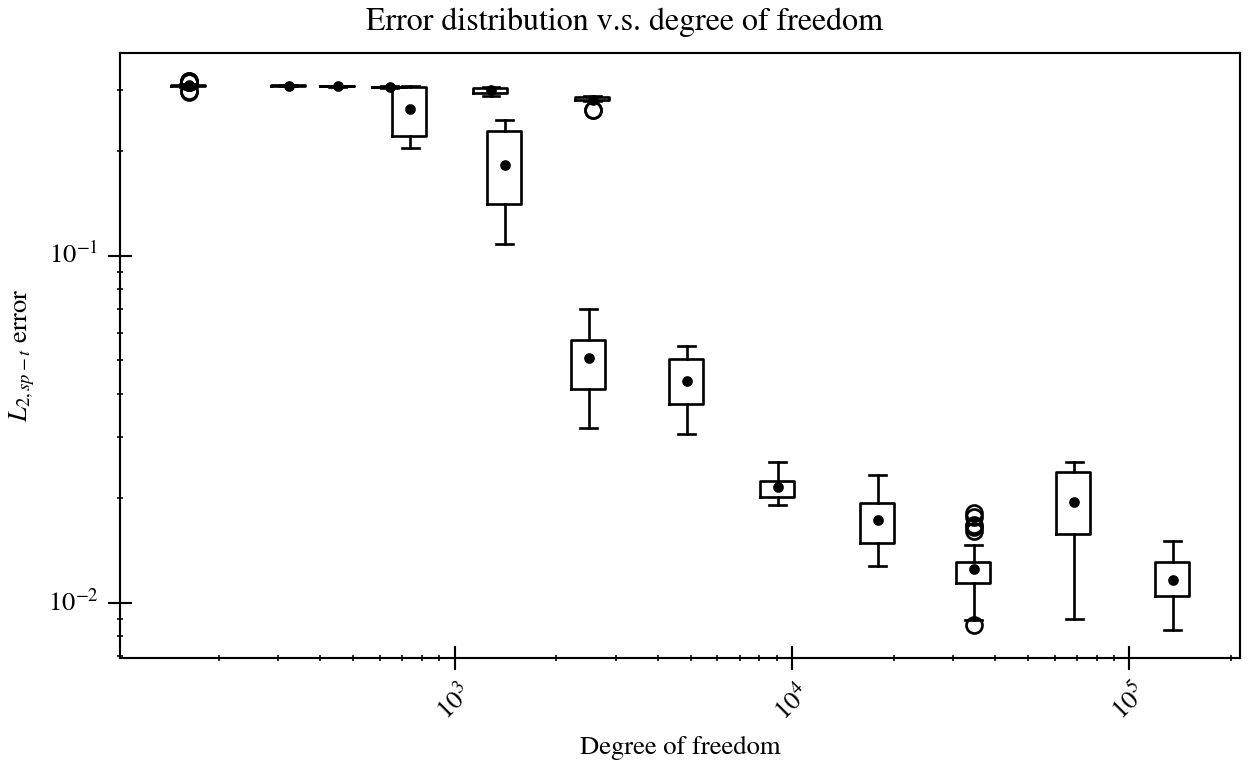
\includegraphics[width=0.95\linewidth]{tgv-2d-re100/err-vs-model-complexity/err-dof-boxplot}
    \caption[%
        PINNs, 2D TGV, $Re=100$: $L_{2,sp-t}$ error v.s. degree of freedom%
    ]{%
        PINNs, 2D TGV, $Re=100$: $L_{2,sp-t}$ error v.s. degree of freedom%
    }
    \label{fig:tgv2d-re100-err-vs-dof}
\end{figure}
From the left portion of the figure, it is obvious that the same number of degrees of freedom does not necessarily give the same accuracy, meaning the model complexity in PINNs can not simply be determined by the number of free parameters in a model.
Also, from the right part of the figure, though increasing the degrees of freedom generally improves the errors, the relationship does not seem to follow a simple monotonically decreasing relationship.
Again, this means the model complexity in PINNs and hence the capability to approximate a complicated flow solution can not be simply determined by the number of free parameters.
This observation also supports the finding that increasing $N_l$ and doubling $N_n$ may have the same effect on the error levels, as the two strategies result in very different numbers of free parameters.

Due to the nonlinearity of PINNs, it is reasonable that the number of free parameters can not be used as a single indicator for how complex an MLP model is.
And to our best knowledge, we have not seen approaches to quantitatively estimate the model complexity.
However, lacking a rigorous understanding of how to evaluate the model complexity in PINNs means, when using PINNs for CFD applications, engineers may not be able to estimate how complicated their PINN models should be to achieve a desired performance.
It further makes it difficult for engineers to evaluate workload, required resources, and costs for engineering projects.

Lastly, figure \ref{fig:tgv2d-re100-err-vs-time} shows the $L_{2,sp-t}$ errors with respect to run times of all cases.
\begin{figure}[hbt!]
    \centering%
    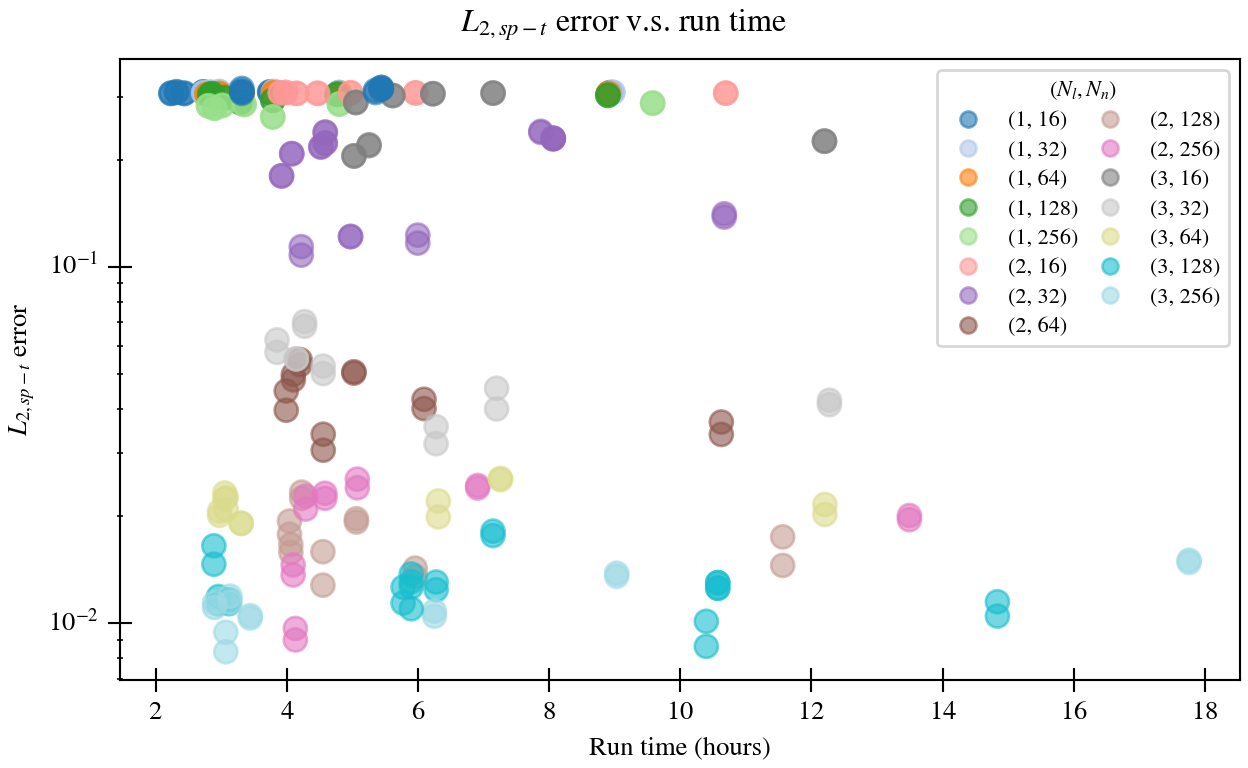
\includegraphics[width=0.95\linewidth]{tgv-2d-re100/err-vs-time/err-time}
    \caption[%
        PINNs, 2D TGV, $Re=100$: $L_{2,sp-t}$ error v.s. run time%
    ]{%
        PINNs, 2D TGV, $Re=100$: $L_{2,sp-t}$ error v.s. run time%
    }
    \label{fig:tgv2d-re100-err-vs-time}
\end{figure}
The colors of dots represent different architectures.
We observed that dots with the same colors are roughly at the same level of errors but are distributed across a wide range of $x$-axis.
It indicates that while $N_{bs}$ has a strong impact on the time costs, it does not have an evident effect on the accuracy.
We did not expect this result because, traditionally in deep learning, using more training data per batch gives a faster convergence and prediction accuracy.
More data per batch means the statistical properties are similar across different batches, and thus the hypersurface does not change significantly from iteration to iteration.
One explanation to the figure \ref{fig:tgv2d-re100-err-vs-time} is that our test cases used too many training points.
The smallest case, $N_{bs}=1024$, might still be big enough for this TGV problem and hence we were not able to see the effect of $N_{bs}$ in the accuracy and convergence rates.
Another explanation is that PINNs are generally insensitive to $N_{bs}$. 
Unfortunately, our test cases are not able to confirm either claim at this point.
If we strictly follow our benchmark results, increasing $N_{bs}$ simply increases the time costs without providing any benefit.
% vim:ft=tex


    \subsection{Training Strategy Investigation}
    \label{sec:pinn-2d-tgv-training-strategy}
    %! TEX root = main.tex
This subsection presents our experiments with several new training strategies, including the annealing loss aggregation, cyclical learning rate, stochastic weight averaging, and the nonlinear conjugate-gradient method.

\subsubsection{Annealing Loss Aggregation}

We applied annealing loss aggregation described in section \ref{sec:loss-annealing} to the cases of $(N_l, N_n, N_{bs}) = (1, 16, 8192)$, $(2, 32, 8192)$, and $(3, 128, 8192)$.
The $\lambda$ parameter in the annealing algorithm is $0.1$ for all cases.
In all the comparisons, we refer to the original loss handling (i.e., equation \eqref{eq:total-residual}) as {\it even-weight aggregation} in the text and {\it naive sum} in the figures to save space.

\begin{figure}[hbt!]
    \centering%
    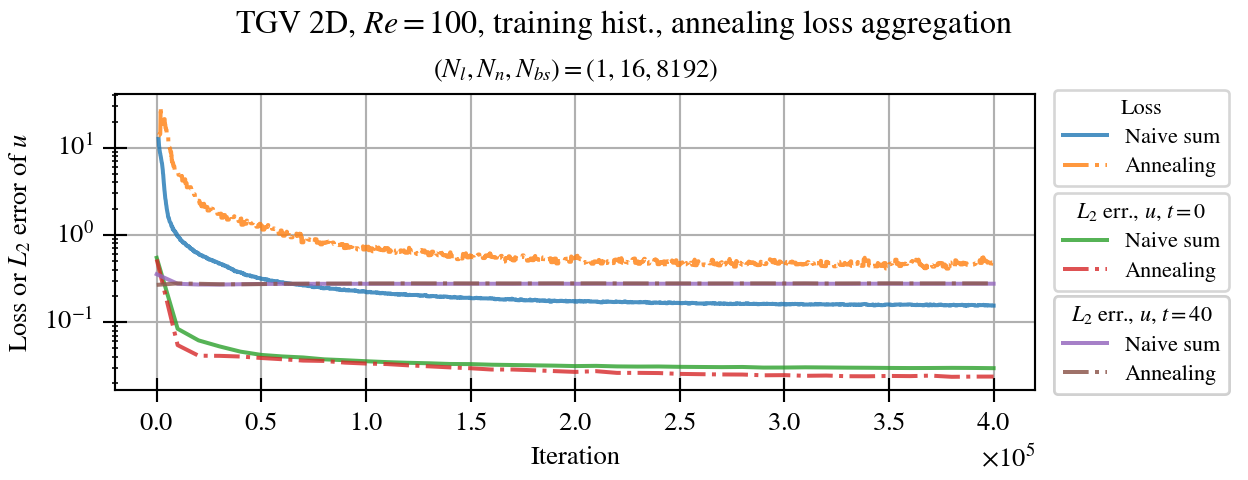
\includegraphics[width=0.9\linewidth]{tgv-2d-re100/annealing-tests/nl1-nn16-npts8192-steps}%
    \caption[%
        Annealing loss aggregation: loss and $L_2$ errors of $u$ v.s. iteration ($(N_l, N_n, N_{bs})=(1, 16, 8192)$)%
    ]{%
        Annealing loss aggregation: loss and $L_2$ errors of $u$ v.s. iteration ($(N_l, N_n, N_{bs})=(1, 16, 8192)$)%
    }\label{fig:annealing-tests-nl1-nn16-npts8192-steps}%
\end{figure}

\begin{figure}[hbt!]
    \centering%
    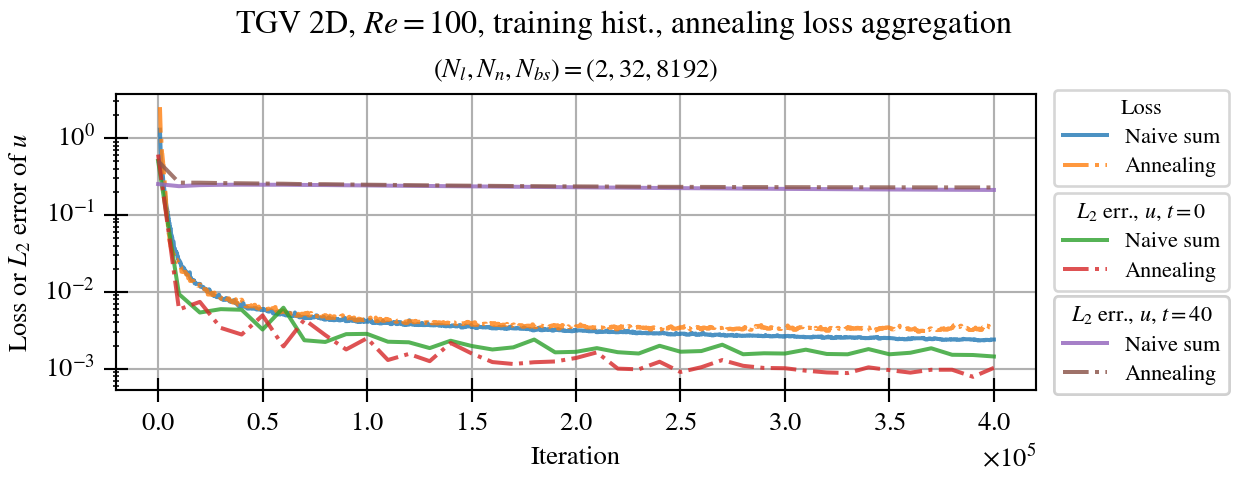
\includegraphics[width=0.9\linewidth]{tgv-2d-re100/annealing-tests/nl2-nn32-npts8192-steps}%
    \caption[%
        Annealing loss aggregation: loss and $L_2$ errors of $u$ v.s. iteration ($(N_l, N_n, N_{bs})=(2, 32, 8192)$)%
    ]{%
        Annealing loss aggregation: loss and $L_2$ errors of $u$ v.s. iteration ($(N_l, N_n, N_{bs})=(2, 32, 8192)$)%
    }\label{fig:annealing-tests-nl2-nn32-npts8192-steps}%
\end{figure}

\begin{figure}[hbt!]
    \centering%
    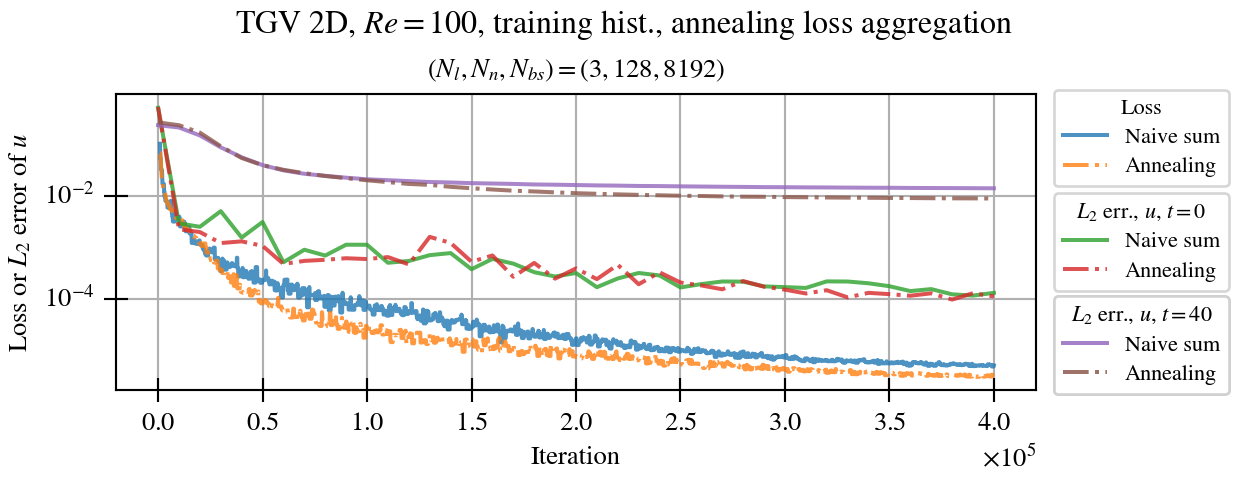
\includegraphics[width=0.9\linewidth]{tgv-2d-re100/annealing-tests/nl3-nn128-npts8192-steps}%
    \caption[%
        Annealing loss aggregation: loss and $L_2$ errors of $u$ v.s. iteration ($(N_l, N_n, N_{bs})=(3, 128, 8192)$)%
    ]{%
        Annealing loss aggregation: loss and $L_2$ errors of $u$ v.s. iteration ($(N_l, N_n, N_{bs})=(3, 128, 8192)$)%
    }\label{fig:annealing-tests-nl3-nn128-npts8192-steps}%
\end{figure}

Figures \ref{fig:annealing-tests-nl1-nn16-npts8192-steps}, \ref{fig:annealing-tests-nl2-nn32-npts8192-steps}, and \ref{fig:annealing-tests-nl3-nn128-npts8192-steps} show the convergence histories of the aggregated losses and errors of $u$.
An interesting observation is that, in figure \ref{fig:annealing-tests-nl1-nn16-npts8192-steps}, the evident gap in the losses of the two algorithms are not reflected in the errors of $u$.
The reason may be that the difference in the losses is due to the different weights of loss terms.
Annealing aggregation may assign a large weight to the IC loss and hence shows a higher aggregated loss.
Other than this observation, we did not observe quantitatively significant difference in both loss and errors between the two algorithms.

Figure \ref{fig:annealing-tests-final-sterrs} gives the comparison of the final $L_{2,sp-t}$ for both $u$ and $v$ velocity.
For simpler network architectures, $(1, 16, 8192)$ and $(2, 32, 8192)$, the final spatial-temporal errors are close.
The more complicated model, $(3, 128, 8192)$, shows visually obvious difference.
However, after examining the actual quantities, we consider them similar.
For example, in the $u$ velocity and with the case of $(3, 128, 8192)$, the even-weight aggregation has an error between $1e-2$ to $2e-2$, while the annealing algorithm has an error between $8e-3$ to $9e-3$.
The difference is just about $20\%$ smaller relative to the even-weight aggregation.
And this difference is even smaller in $v$ velocity.

\begin{figure}[hbt!]
    \centering%
    \includegraphics[width=0.9\linewidth]{tgv-2d-re100/annealing-tests/final-spatial-temporal-errors}%
    \caption[%
        Annealing loss aggregation: final spatial-temporal errors%
    ]{%
        Annealing loss aggregation: final spatial-temporal errors%
    }\label{fig:annealing-tests-final-sterrs}%
\end{figure}

We further examined the convergence with respect to the run times.
Annealing loss aggregation is more expensive as it involves evaluating the gradient of each single loss term with respect to model parameters.
As shown in figures \ref{fig:annealing-tests-nl1-nn16-npts8192-walltimes}, \ref{fig:annealing-tests-nl2-nn32-npts8192-walltimes}, and \ref{fig:annealing-tests-nl3-nn128-npts8192-walltimes}, the even-weight aggregation is considered to converge much faster in terms of the run time.
Though annealing aggregation shows a slightly better accuracy at the end of training for $(3, 128, 8192)$, the even-weight aggregation achieves slightly better losses and errors under a given, meaning a better accuracy-cost ratio.
Annealing loss aggregation's computational cost is about the double of the even-weight aggregation. 

\begin{figure}[hbt!]
    \centering%
    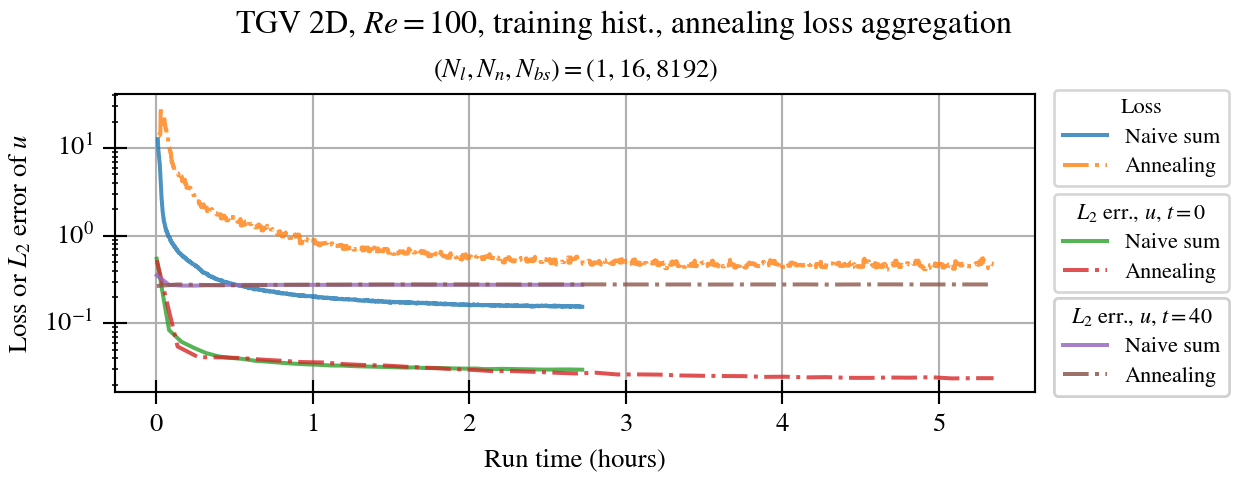
\includegraphics[width=0.9\linewidth]{tgv-2d-re100/annealing-tests/nl1-nn16-npts8192-walltimes}%
    \caption[%
        Annealing loss aggregation: loss and $L_2$ errors of $u$ v.s. wall time ($(N_l, N_n, N_{bs})=(1, 16, 8192)$)%
    ]{%
        Annealing loss aggregation: loss and $L_2$ errors of $u$ v.s. wall time ($(N_l, N_n, N_{bs})=(1, 16, 8192)$)%
    }\label{fig:annealing-tests-nl1-nn16-npts8192-walltimes}%
\end{figure}

\begin{figure}[hbt!]
    \centering%
    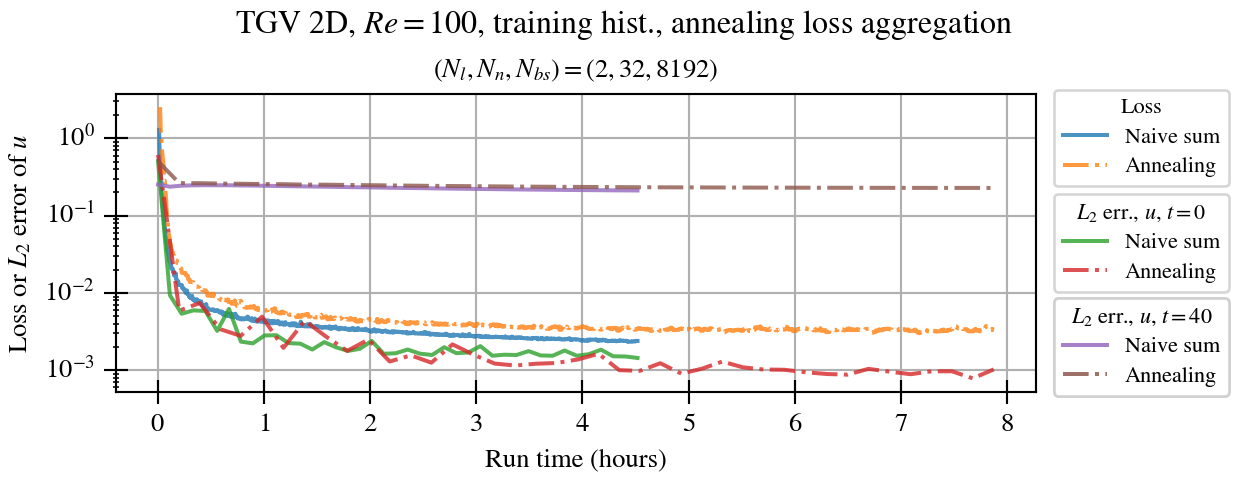
\includegraphics[width=0.9\linewidth]{tgv-2d-re100/annealing-tests/nl2-nn32-npts8192-walltimes}%
    \caption[%
        Annealing loss aggregation: loss and $L_2$ errors of $u$ v.s. wall time ($(N_l, N_n, N_{bs})=(2, 32, 8192)$)%
    ]{%
        Annealing loss aggregation: loss and $L_2$ errors of $u$ v.s. wall time ($(N_l, N_n, N_{bs})=(2, 32, 8192)$)%
    }\label{fig:annealing-tests-nl2-nn32-npts8192-walltimes}%
\end{figure}

\begin{figure}[hbt!]
    \centering%
    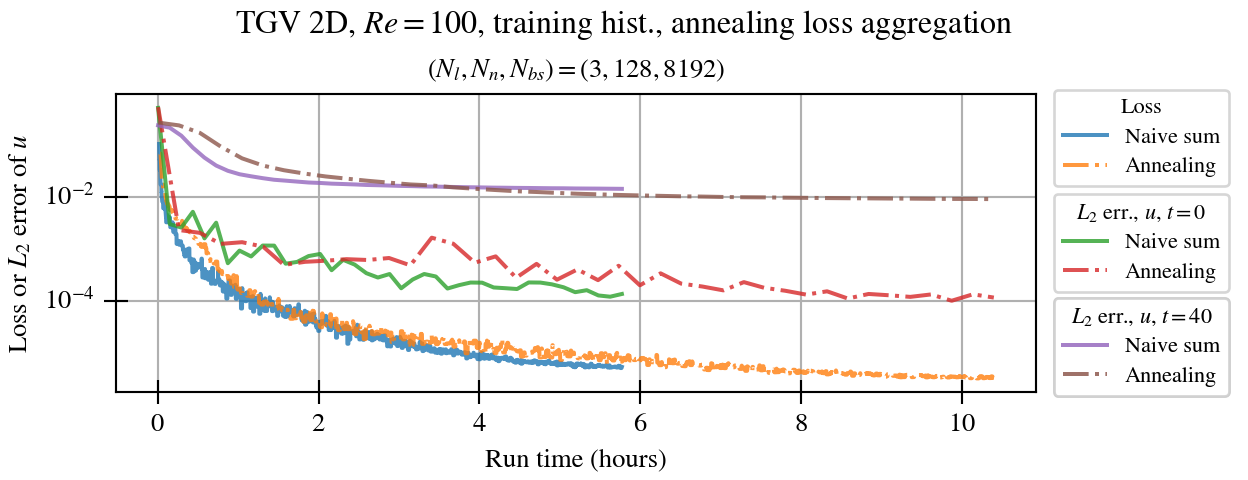
\includegraphics[width=0.9\linewidth]{tgv-2d-re100/annealing-tests/nl3-nn128-npts8192-walltimes}%
    \caption[%
        Annealing loss aggregation: loss and $L_2$ errors of $u$ v.s. wall time ($(N_l, N_n, N_{bs})=(3, 128, 8192)$)%
    ]{%
        Annealing loss aggregation: loss and $L_2$ errors of $u$ v.s. wall time ($(N_l, N_n, N_{bs})=(3, 128, 8192)$)%
    }\label{fig:annealing-tests-nl3-nn128-npts8192-walltimes}%
\end{figure}

\subsubsection{Cyclical Learning Rate and Stochastic Weight Averaging}

The benchmarks in this section cover the cyclical learning rate and stochastic weight averaging (SWA).
The cyclical learning rate (equation \eqref{eq:cyclical-learning-rate}) in this section was configured with $\eta_{low}=1.5e-5$, $\eta_{high}=1.5e-3$, $N_c=5000$, and $\gamma=0.999989$.
Figure \ref{fig:cyclic-swa-tests-lr-hist} shows a comparison of the learning rate from the original exponentially-decaying and the cyclical learning rate.
\begin{figure}[hbt!]
    \centering%
    \includegraphics{tgv-2d-re100/cyclic-swa-tests/learning-rate-hist}%
    \caption[%
        Cyclical LR and SWA: learning rate history%
    ]{%
        Cyclical LR and SWA: learning rate history%
    }\label{fig:cyclic-swa-tests-lr-hist}%
\end{figure}
The exponentially-decaying learning rate will be simply denoted as {\it exponential} learning rate in the later discussion and figures.
SWA, on the other, hand, runs in parallel when using cyclical learning rate and does not affect the normal training process.
It is thus able to decouple the performance of SWA from the results of only cyclical learning rate.
In the cases presented here, SWA was configured to collect and average the model parameters from the last 200,000 iterations of the training.
Its results share the same convergence histories with the cases of pure cyclical learning rates.
The only difference between with and without SWA lies in the prediction errors (e.g., errors in $u$) after iteration 200,000.

\begin{figure}[hbt!]
    \centering%
    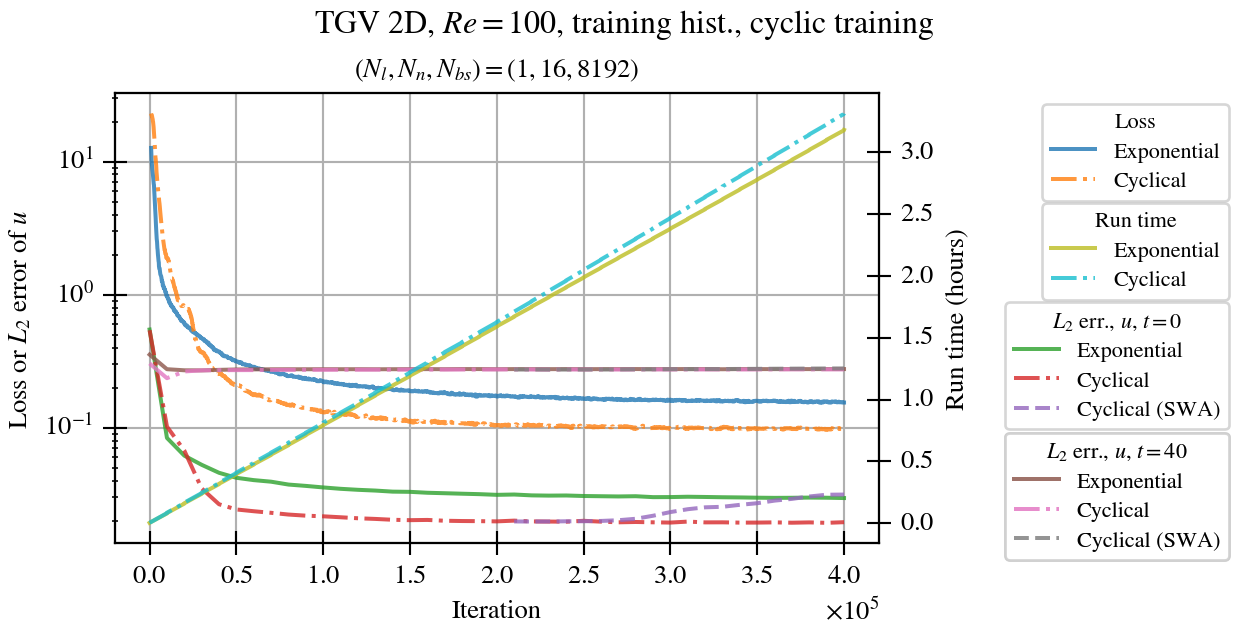
\includegraphics[width=0.9\linewidth]{tgv-2d-re100/cyclic-swa-tests/nl1-nn16-npts8192}%
    \caption[%
        Cyclical LR and SWA: loss and $L_2$ errors of $u$ v.s. iteration ($(N_l, N_n, N_{bs})=(1, 16, 8192)$)%
    ]{%
        Cyclical LR and SWA: loss and $L_2$ errors of $u$ v.s. iteration ($(N_l, N_n, N_{bs})=(1, 16, 8192)$)%
    }\label{fig:cyclic-swa-tests-nl1-nn16-npts8192}%
\end{figure}

\begin{figure}[hbt!]
    \centering%
    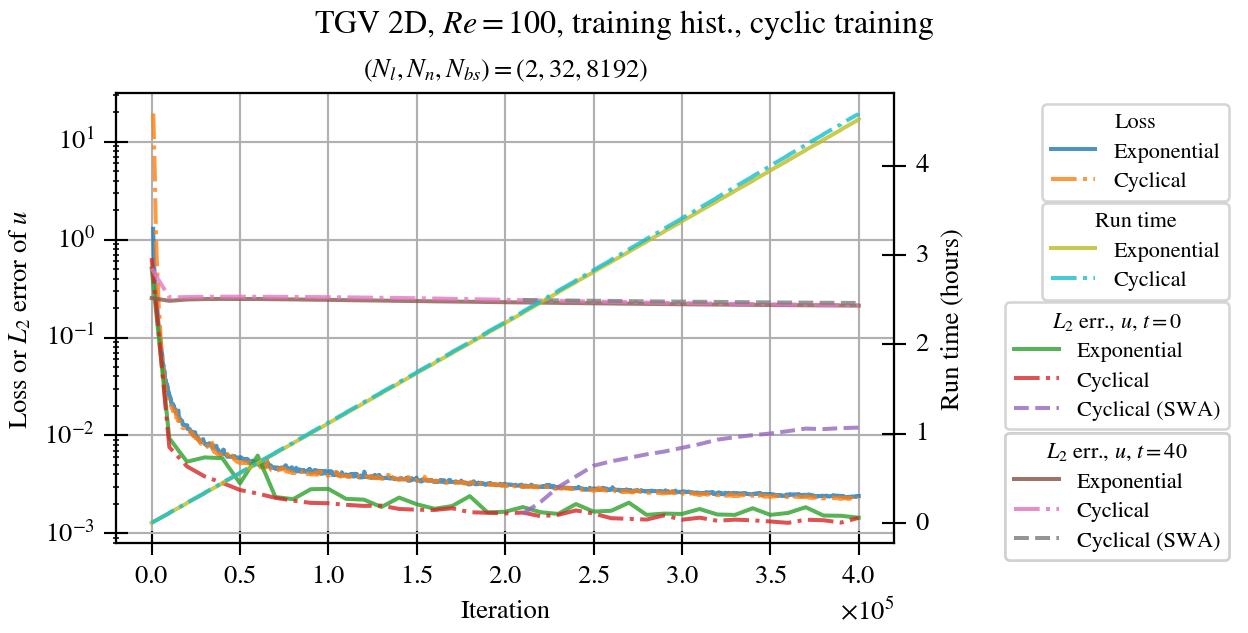
\includegraphics[width=0.9\linewidth]{tgv-2d-re100/cyclic-swa-tests/nl2-nn32-npts8192}%
    \caption[%
        Cyclical LR and SWA: loss and $L_2$ errors of $u$ v.s. iteration ($(N_l, N_n, N_{bs})=(2, 32, 8192)$)%
    ]{%
        Cyclical LR and SWA: loss and $L_2$ errors of $u$ v.s. iteration ($(N_l, N_n, N_{bs})=(2, 32, 8192)$)%
    }\label{fig:cyclic-swa-tests-nl2-nn32-npts8192}%
\end{figure}

\begin{figure}[hbt!]
    \centering%
    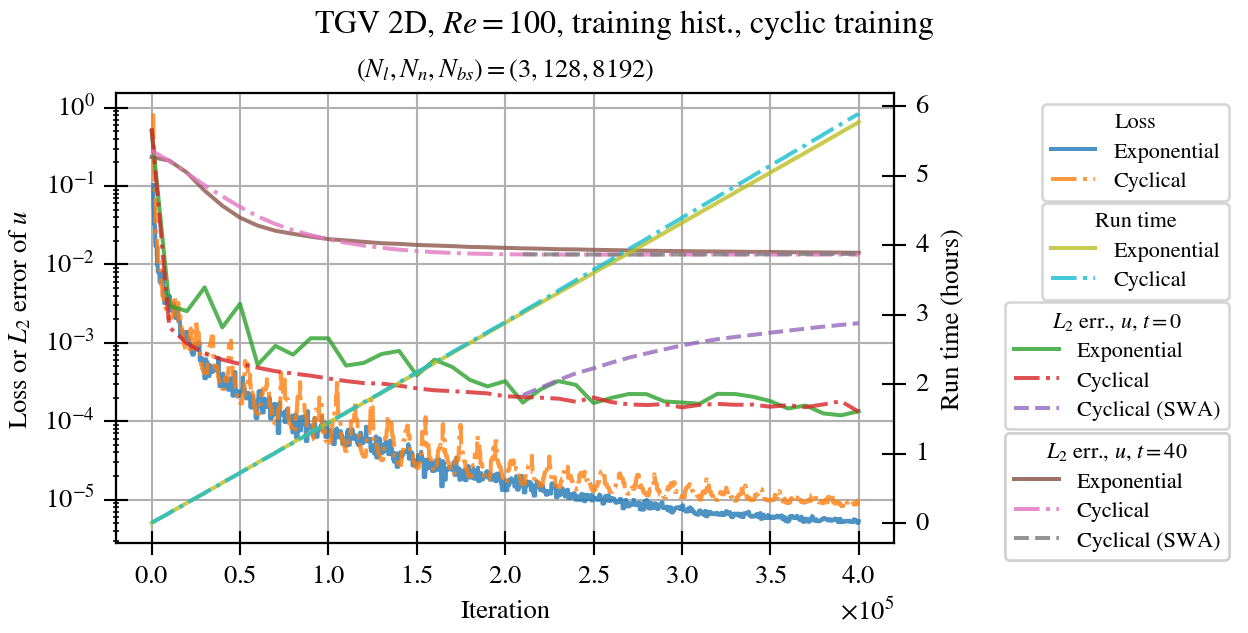
\includegraphics[width=0.9\linewidth]{tgv-2d-re100/cyclic-swa-tests/nl3-nn128-npts8192}%
    \caption[%
        Cyclical LR and SWA: loss and $L_2$ errors of $u$ v.s. iteration ($(N_l, N_n, N_{bs})=(3, 128, 8192)$)%
    ]{%
        Cyclical LR and SWA: loss and $L_2$ errors of $u$ v.s. iteration ($(N_l, N_n, N_{bs})=(3, 128, 8192)$)%
    }\label{fig:cyclic-swa-tests-nl3-nn128-npts8192}%
\end{figure}

In figures \ref{fig:cyclic-swa-tests-nl1-nn16-npts8192}, \ref{fig:cyclic-swa-tests-nl2-nn32-npts8192}, and \ref{fig:cyclic-swa-tests-nl3-nn128-npts8192}, we presented the convergence histories and the time costs.
First, the run times between the two learning rate strategies are similar.
This is expected as cyclical learning rate does not add notable operations to the training.

We next examined the convergence of cyclical and exponentially-decaying learning rates.
The results show that obvious difference only exists in the simplest model, $(1, 16, 8192)$.
However, this difference may be obvious only because the narrower $y$-axis scale in figure \ref{fig:cyclic-swa-tests-nl1-nn16-npts8192}.
If we plot all three figures using the same scale, the difference in $(1, 16, 8192)$ may not be noticeable.
The quantitative difference also supports this claim.
For example, the final loss of exponential learning rate is about $2e-1$, and that of cyclical learning rate is around $1e-1$.
We do not consider this difference significant.

Also, slight oscillation and evident oscillation can be seen in $(2, 32, 8192)$ and $(3, 128, 8192)$, respectively. 
The oscillations may represent how cyclical learning rate helps in escaping local minimums and saddle points. 
The reason that $(1, 16, 8192)$ does not show oscillation may be attributed to the simple hypersurface of $r(\Theta)$.
This architecture may be too simple and may not exhibit complex topography on the hypersurface.

The results in the errors of $u$ show that SWA does not help achieve better predictions at all.
It even hurts the prediction accuracy for $t=0$.
As for $t=40$, for reasons unknown to us at this point, there is no difference.
However, as there is no theory nor guidelines to determine how many iterations should be involved in SWA, the results may be different if using fewer iterations.
Although in this work we did not investigate more on SWA, it could be a potential research question for future studies.

\begin{figure}[hbt!]
    \centering%
    \includegraphics[width=0.9\linewidth]{tgv-2d-re100/cyclic-swa-tests/final-spatial-temporal-errors}%
    \caption[%
        Cyclic LR and SWA: final spatial-temporal errors%
    ]{%
        Cyclic LR and SWA: final spatial-temporal errors%
    }\label{fig:cyclic-swa-tests-final-sterrs}%
\end{figure}

Figure \ref{fig:cyclic-swa-tests-final-sterrs} shows the graphical comparison of the overall spatial-temporal error, $L_{2,sp-t}$.
The results are similar.
Even though SWA gives worse predictions at $t=0$, the integrated error over $t=0$ to $t=100$ does not show significant difference.

\subsubsection{Nonlinear Conjugate-Gradient Optimizer}

The last attempt to adopt new training strategy was the application of nonlinear conjugate-gradient.
The major difficulty of applying CG lies in how to handle batch training.
CG relies on the previous search direction to determine the current search direction, and the former is based on the hypersurface in the last iteration.
In batch training, the hypersurface more or less changes from iteration to iteration due to using different training points.
It is unclear how legit the previous search direction is to be used in the current iteration.

Moreover, in each iteration, the line search algorithm search for a new location along the search direction according to the Wolfe conditions or their derived conditions.
A point meets the Wolfe conditions in the previous iteration does not necessarily meet the same conditions in the current iteration.
This may cause convergence issues in CG as the convergence of CG relies on properly determining the location on each search direction.

Nevertheless, given the efficiencies of CG in non-batched training, we would like to experiment the possibility of using it.
In our current attempt, we used CG to optimize the loss $r(\Theta)$ for a certain batch to a given tolerance before moving on to the next batch.
Also, CG may not have capability to escape from poor local minimums, so our attempts first used Adam for optimization up to 200,000 iterations to identify a region with proper minimum, and then CG was used for an extra 200 iterations.
In other words, pure Adam cases ran 400,000 iterations, while the CG cases ran 200,000 Adam iterations and then 200 iterations with CG.
The case tested are $(1, 16, 8192)$, $(2, 32, 8192)$, and $(3, 128, 8192)$.
CG trained each batch until the change in the loss is smaller than $1e-6$.

\begin{figure}[hbt!]
    \centering%
    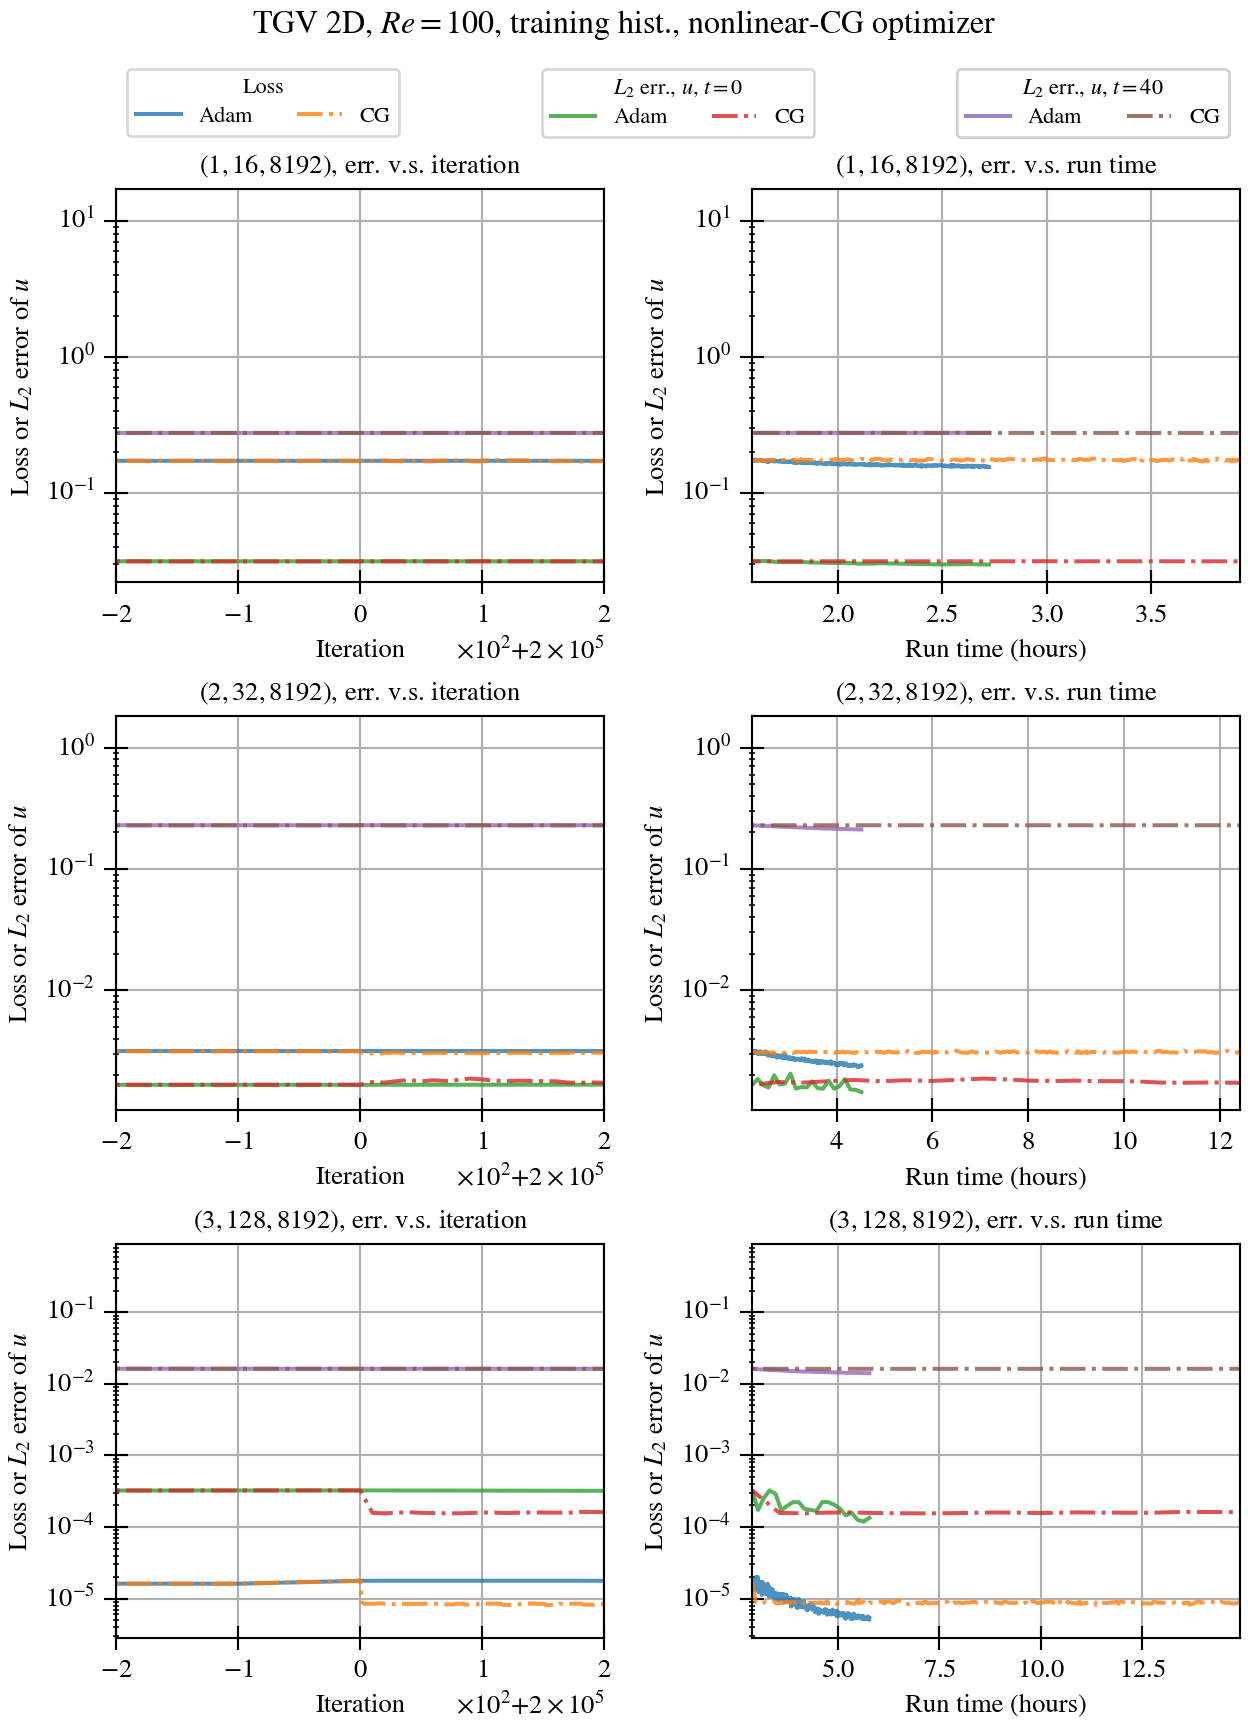
\includegraphics[width=\linewidth]{tgv-2d-re100/ncg-tests/training-hist}%
    \caption[%
        Nonlinear-CG: training history%
    ]{%
        Nonlinear-CG: training history%
    }\label{fig:ncg-tests-train-hist}%
\end{figure}

Figure \ref{fig:ncg-tests-train-hist} shows the comparison of convergence histories between Adam-only cases and CG cases.
On the left we have the losses and errors versus iterations.
The range of iterations shown in the $x$-axis is 199,800th to 200,200th iteration.
We can see for simple architectures, CG does not help reduce the losses.
Based on the observations and discussions in the previous sections, cases with simple architectures converge very early.
It is hence reason for CG not able to improve the losses in simple architectures because they may have already converged.
However, $(3, 128, 8192)$ does show a sudden drop in the loss and error at $t=0$.
After the sudden drop, further training with new batches does not further improve the loss and errors.

On the right of the same figure, we have losses and errors versus run time.
The range of the run time starts from the time for 200,000 iterations until the end of training.
In other words, sub-figures on the right show the 200,000th to 400,000th training iterations for Adam-only cases and 200,000th to 200,200th training iterations for CG cases.
As we use CG on each batch until a certain tolerance, one training iteration with CG consists of hundreds or thousands of sub-iterations inside the CG solver.
Therefore, it is reasonable to see 200 training iterations with CG takes much longer time than 200,000 iterations with Adam.
It is clear from these sub-figures, although CG provides a sudden drop in the losses, it does not further improve the training.
And eventually, Adam reaches even smaller losses than CG does.
More importantly, Adam take much less time.

\begin{figure}[hbt!]
    \centering%
    \includegraphics[width=0.9\linewidth]{tgv-2d-re100/ncg-tests/final-spatial-temporal-errors}%
    \caption[%
        Nonlinear-CG: overall spatial-temporal errors%
    ]{%
        Nonlinear-CG: overall spatial-temporal errors%
    }\label{fig:ncg-tests-final-sterrs}%
\end{figure}

Figure \ref{fig:ncg-tests-final-sterrs} shows the final spatial-temporal errors of $u$ and $v$ velocity.
CG does not provide more accurate results.

As mentioned, the major problem with CG is the combined use with batch training and the capability to escape from saddle points and poor minimums.
Carefully tuned line search parameters and algorithm may help achieve the escaping.
However, how to deal with batched training is still a question.
If the issues is caused by the change in hypersurface, then using more training points per batch may help stabilize the hypersurface from iteration to iteration.
And hence each CG iteration is itself a training iteration, i.e., each batch of points is used in one CG iteration.
This may be a potential direction for future investigation on this topic.
% vim:ft=tex

\section{Steady 2D Cylinder Flow: \texorpdfstring{$Re=40$}{re40}}
\label{sec:pinn-2d-cylinder-re40}

    \subsection{Problem Description and Configurations}
    \label{sec:pinn-2d-cylinder-re40-conf}
    %! TEX root = main.tex
The second part of our benchmarking with PINNs focuses on the ability to simulate nonlinear dynamical systems of flow problems.
Our benchmark target is the 2D cylinder flow at $Re=200$, which exhibits vortex shedding.
However, before we conduct the $Re=200$ cylinder flow test, we would like to test a steady cylinder flow problem with our unsteady PINN implementation for solver validation.
The selected case is $Re=40$ cylinder flow, which reaches a steady state eventually.
The results were validated with experimental data and verified against PetIBM results.

The computational domain of the $Re=40$ cylinder flow is $[-10$, $30]$ $\times$ $[-10$, $10]$, and the simulation time range is $t=0$ to $t=20$.
A cylinder with a radius of $0.5$ sits at the coordinate $(0$, $0)$.
Nondimensional density is $1$, and kinematic viscosity is $0.025$, so the Reynolds number is $40$.
The IC is $u=1$ and $v=0$.
The BCs are $u=1$ and $v=0$ on $x=-10$, $y=-10$, and $y=10$.
The BC at the outlet $x=30$ is a 1D convective condition:
\begin{equation}\label{eq:convec-bc}
    \left\{
    \begin{aligned}
        &\pdiff{u}{t} + c\pdiff{u}{\vec{n}} = 0 \\
        &\pdiff{v}{t} + c\pdiff{v}{\vec{n}} = 0 \\
    \end{aligned}
    \right.
\end{equation}
where $\vec{n}$ is the normal vector of the boundary pointing outward from the domain, and $c$ is the convection speed.
In this work, we used $c=1$.

The network used is $(N_l$, $N_n)$ $=$ $(6$, $512)$.
Two PINN implementations were used: a steady solver and an unsteady one.
Two different $N_{bs}$ were used as well to confirm the effect of batch sizes we observed in the previous section: $N_{bs}=\num{6400}$ and $N_{bs}=\num{25600}$.
And we tested two different cyclical learning rate configurations:
\begin{enumerate}[nolistsep]
    \item Large cycle: $(\eta_{low}, \eta_{high}, N_c, \gamma)=(1\times 10^{-6},\ 1\times 10^{-2},\ 5000,\ 0.99998)$
    \item Small cycle: $(\eta_{low}, \eta_{high}, N_c, \gamma)=(1\times 10^{-6},\ 1\times 10^{-3},\ 2000,\ 0.999972)$
\end{enumerate}
Figure \ref{fig:cylinder-2d-re40-lr-hist} shows the comparison of the two schedules.
\begin{figure}[hbt!]
    \includegraphics[width=0.9\linewidth]{cylinder-2d-re40/learning-rate-hist}
    \caption[%
        PINNs, 2D Cylinder, $Re=40$: cyclical learning rate configurations%
    ]{%
        PINNs, 2D Cylinder, $Re=40$: cyclical learning rate configurations%
    }%
    \label{fig:cylinder-2d-re40-lr-hist}
\end{figure}
A total of 6 cases were run in this benchmark.
(The small cyclical schedule was not applied to $N_{bs}=\num{25600}$.)

For unsteady cases with $N_{bs}=\num{6400}$, the PINN solver sampled $\num{6400}\times \num{10000}$ points from the computational spatial-temporal domain for PDE losses, meaning each batch was repeated every $\num{10000}$ iterations.
Except for the cylinder surface, $640\times \num{10000}$ points were sampled on each boundary and $t\in[0$, $20]$.
On the cylinder surface, $256\times \num{10000}$ points were sampled and also with $t\in[0$, $20]$.
To evaluate IC losses, $\num{6400}\times \num{10000}$ points were sampled from the spatial domain with their temporal coordinates being constrained to $t=0$.
The steady cases with $N_{bs}=\num{6400}$ follows a similar setting, except the PDE evaluation points were sampled only from spatial domain, as there was no temporal coordinates.
And steady cases did not need to evaluate IC losses.

For cases with $N_{bs}=\num{25600}$, the PDE evaluation points follow the same logic described above.
We used $\num{2560}\times \num{10000}$ points on the boundaries of $y=\pm 10$ and $\num{1280}\times \num{10000}$ points on the boundaries of $x=-10$ and $x=30$.
The cylinder surface had $512\times \num{10000}$ points.

Each case ran for \num{400000} iterations during optimization with the Adam optimizer.
The hardware used was 1 NVIDIA A100 GPU for all cases.

A PetIBM simulation was done as a baseline.
The simulation ran with an NVIDIA K40 GPU with 6 cores of Intel i7-5930K.
Note that the K40 GPU is 5 generations behind the A100 GPU in terms of the technology specification.
The PetIBM simulation resolved the flow on a $562 \times 447$ stretched Cartesian grid with the same computational spatial-temporal domain.
PetIBM used double-precision floats, while PINNs used single precision floats.
The tolerance for all linear solvers in PetIBM was $\num{1e-14}$.
% vim:ft=tex


    \subsection{Results}
    \label{sec:pinn-2d-cylinder-re40-results}
    %! TEX root = main.tex

For steady cases, the PINN solver took about 25 hours to finish for $N_{bs}=25,600$ and 13.5 hours for $N_{bs}=6,400$.
The steady PINN solver, on the other hand, took about 26 hours and 14.5 hours for $N_{bs}=25,600$ and $6,400$, respectively.
The baseline PetIBM simulation was finished within 2 minutes.

Figure \ref{fig:cylinder-2d-re40-loss-hist-steady} shows the convergence history of the aggregated losses for the steady cases, and figure \ref{fig:cylinder-2d-re40-loss-hist-unsteady} shows those for the unsteady cases.
Each figure includes sub-figures for losses against iterations and run times.
\begin{figure}[hbt!]
    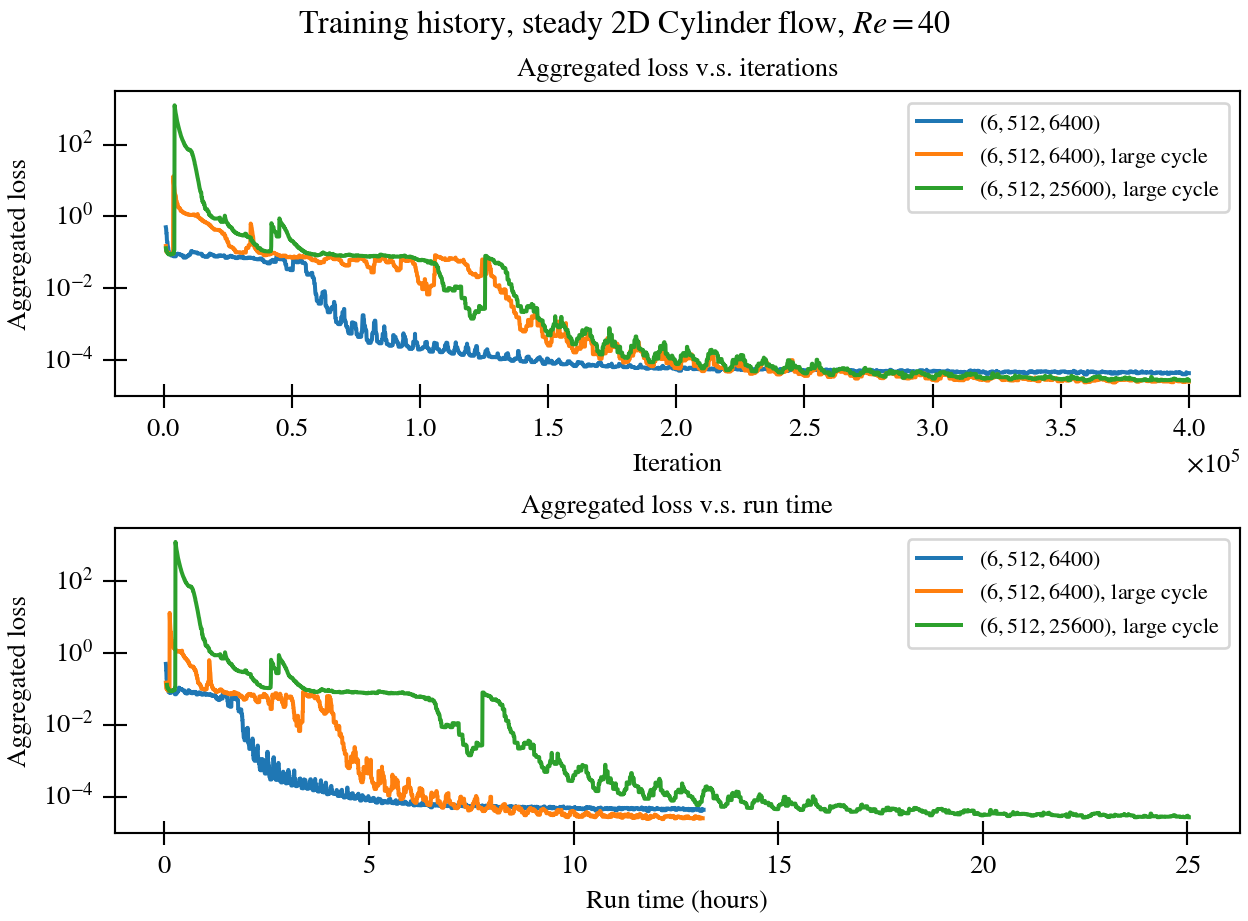
\includegraphics[width=0.9\linewidth]{cylinder-2d-re40/loss-hist-steady}
    \caption[
        PINNs, 2D Cylinder, $Re=40$: training history of steady solvers%
    ]{%
        PINNs, 2D Cylinder, $Re=40$: training history of steady solvers%
    }%
    \label{fig:cylinder-2d-re40-loss-hist-steady}
\end{figure}
\begin{figure}[hbt!]
    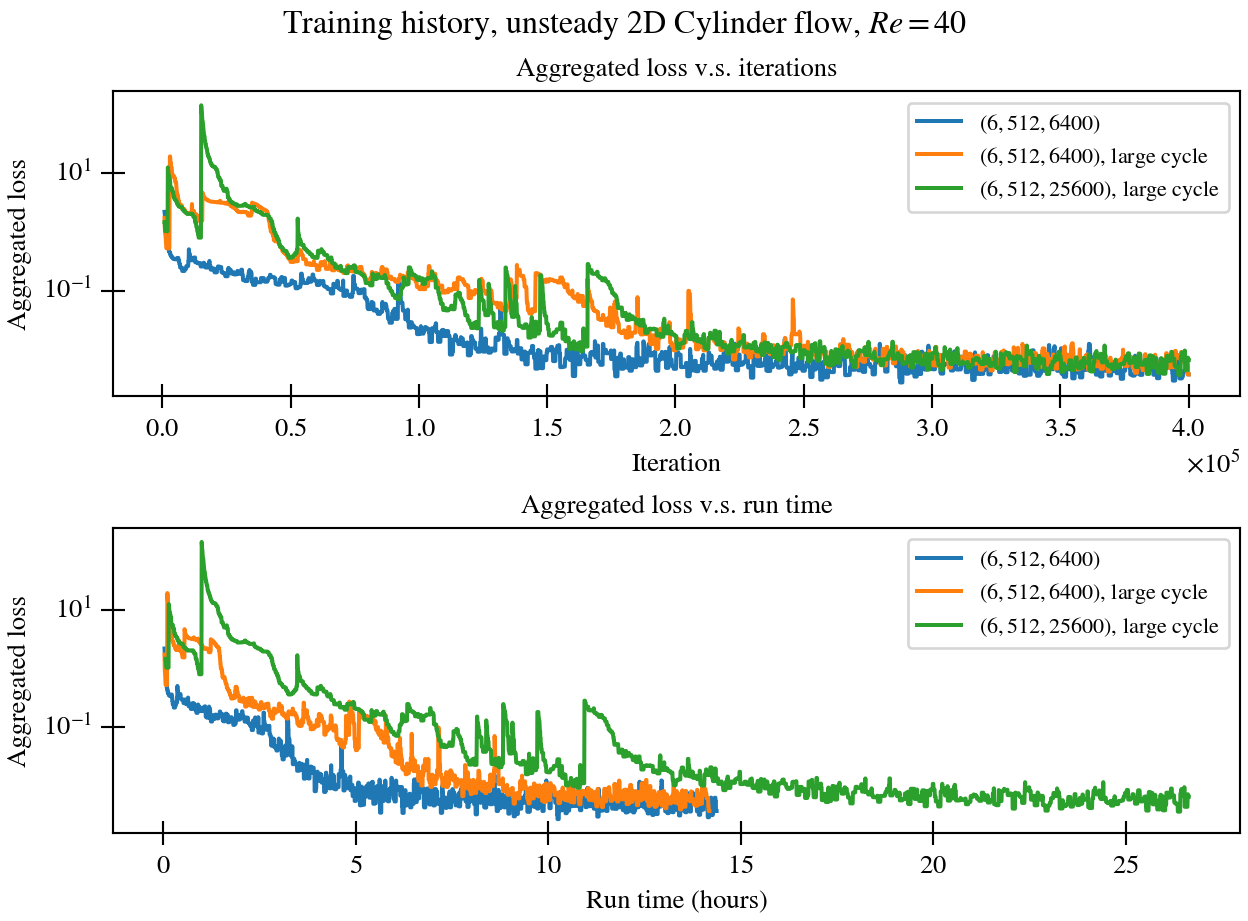
\includegraphics[width=0.9\linewidth]{cylinder-2d-re40/loss-hist-unsteady}
    \caption[
        PINNs, 2D Cylinder, $Re=40$: training history of unsteady solvers%
    ]{%
        PINNs, 2D Cylinder, $Re=40$: training history of unsteady solvers%
    }%
    \label{fig:cylinder-2d-re40-loss-hist-unsteady}
\end{figure}
An interesting observation from figure \ref{fig:cylinder-2d-re40-loss-hist-steady} is the plateaus at the beginning of the training.
Though without a proof, we suspect this trend reflects the escaping from saddle points.
The large cyclical scheduling took more time to escape because it had fewer cycles under given iterations.
Regardless of the difference at the beginning, all cases reaches the same level of losses eventually.
And for the large cyclical scheduling, both $N_{bs}=6,400$ and $N_{bs}=25,600$ show similar convergence history in terms of iterations.
This observation again proves our suspicion in the previous section that $N_{bs}$ does not have significant influence on the losses and errors..

Figure \ref{fig:cylinder-2d-re40-loss-hist-unsteady} also shows plateaus at the beginning, though not as obvious as those for the steady cases.
The convergence histories for the unsteady cases are also bumpier.
We also suspect that it is caused by escaping from saddle points and poor local minimums.
The hypersurface of unsteady solver might be more complicated than the steady one, hence causing more oscillating convergence.
Nevertheless, all unsteady cases converged to a similar loss level.

Figure \ref{fig:cylinder-2d-re40-contours} shows visual comparisons of the steady-state flow fields.
\begin{figure}[hbt!]
    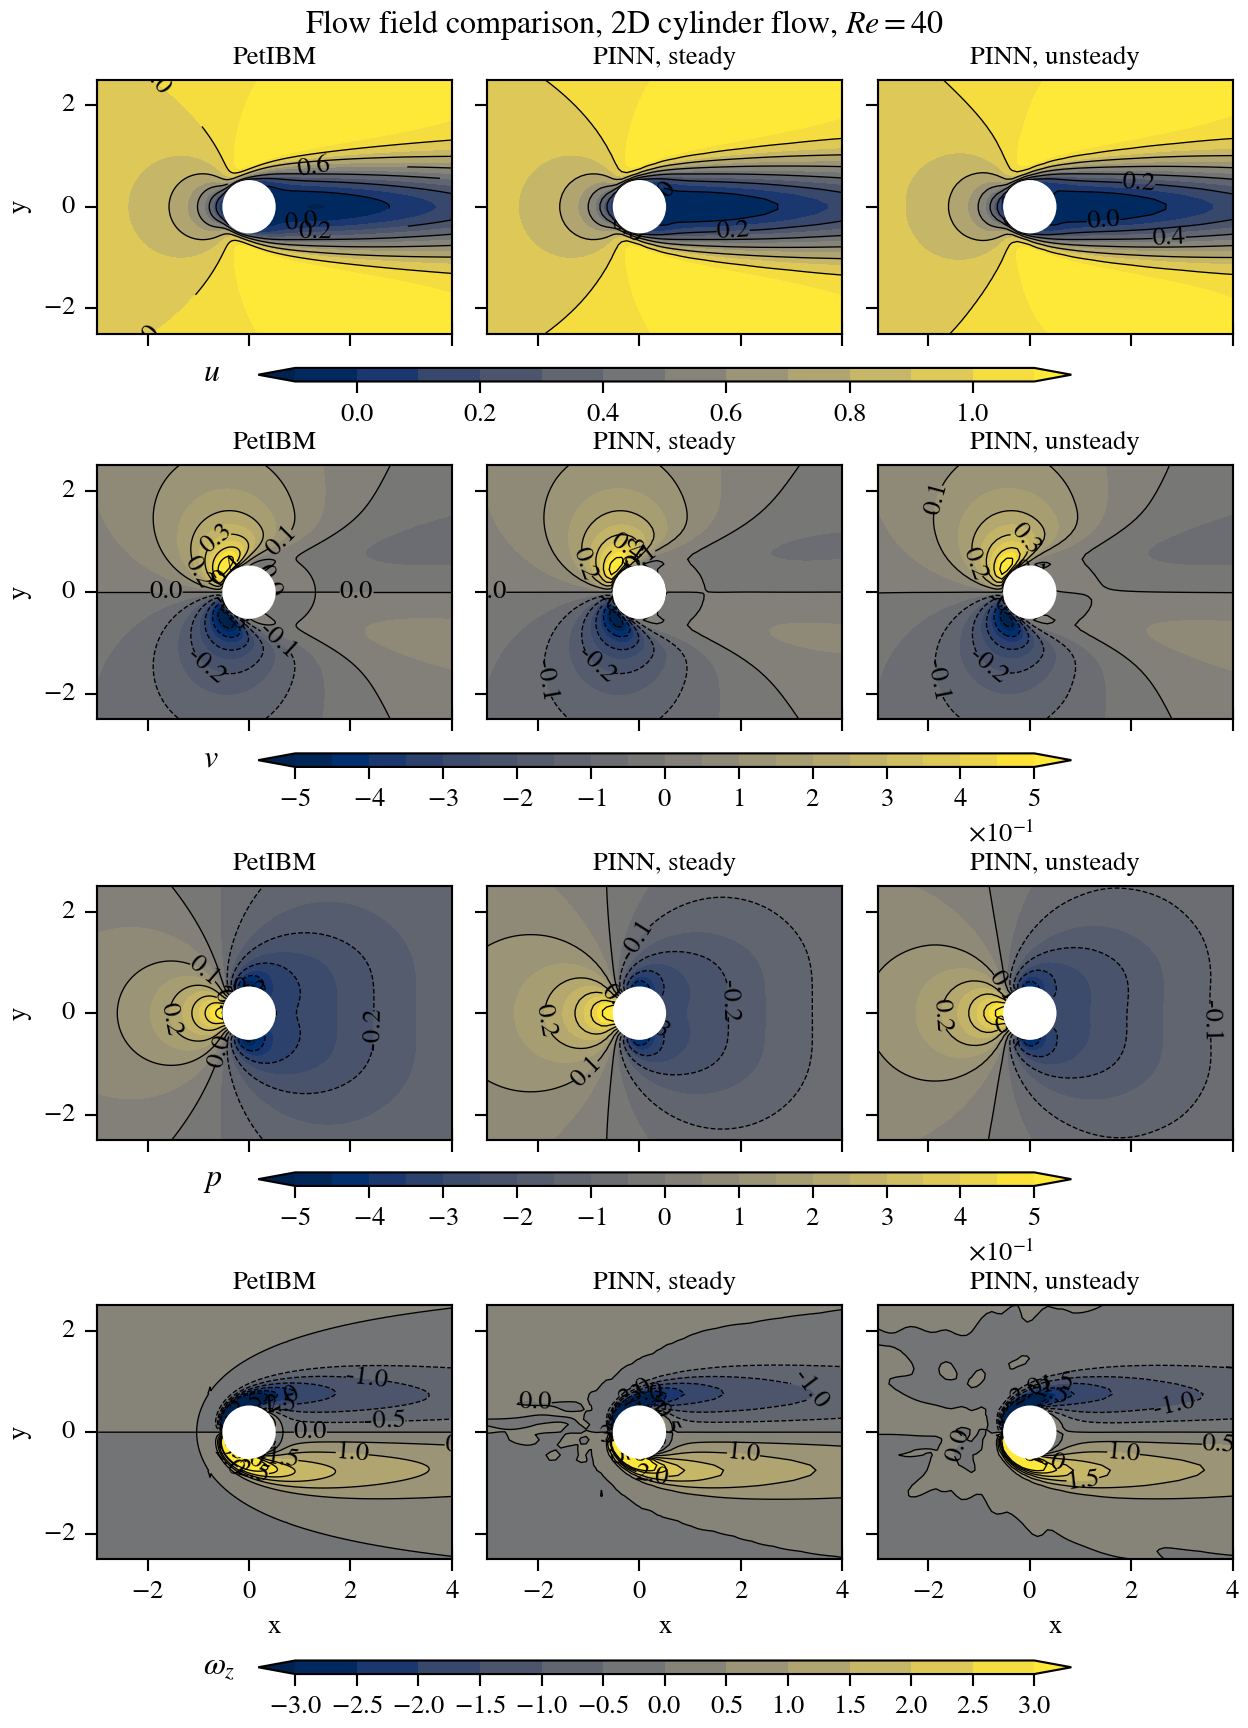
\includegraphics[width=\linewidth]{cylinder-2d-re40/contour-comparison}
    \caption[
        PINNs, 2D Cylinder, $Re=40$: flow fields at steady state%
    ]{%
        PINNs, 2D Cylinder, $Re=40$: flow fields at steady state%
        For the unsteady PINN case, the solution was extracted from $t=20$.
        The fields shown, from the top to bottom, are $u$, $v$, $p$, and vorticity $\omega_z$.
    }%
    \label{fig:cylinder-2d-re40-contours}
\end{figure}
The results of steady PINN solver were obtained from the case of $N_{bs}=25,600$ with the large cyclical scheduling, and that of the unsteady solver was also obtained from the same $N_{bs}$ and scheduling.
All three cases visually agree with each other, except for the vorticity.
Note that vorticity is a product from post-processing for all three solvers.
PetIBM relies on central difference to calculate the vorticity.
And PINNs use automatic differentiation to obtain it.

Figure \ref{fig:cylinder-2d-re40-drag-lift-time} gives the drag and lift coefficients ($C_D$ and $C_L$).
We only plotted the results from the unsteady solver because the steady solvers do not have the time variable. 
\begin{figure}[hbt!]
    \includegraphics[width=\linewidth]{cylinder-2d-re40/drag-lift-coeffs.png}
    \caption[
        PINNs, 2D Cylinder, $Re=40$: drag and lift coefficients%
    ]{%
        PINNs, 2D Cylinder, $Re=40$: drag and lift coefficients%
    }%
    \label{fig:cylinder-2d-re40-drag-lift-time}
\end{figure}
Table \ref{table:cylinder-2d-re40-comparison-cd} compares the values of $C_D$ against the experimental data and simulation data from other groups.
\begin{table}[hbt!]
    \singlespacing
    \begin{threeparttable}[b]
        \begin{tabular}{lccc}
            \toprule
            & $C_D$ & $C_{D_p}$ & $C_{D_f}$ \\
            \midrule
            $(6, 512, 6400)$, steady & 1.62 & 1.07 & 0.55 \\
            $(6, 512, 6400)$, unsteady & 1.63 & 1.02 & 0.61 \\
            $(6, 512, 6400)$, large cycle, steady & 1.62 & 1.07 & 0.55 \\
            $(6, 512, 6400)$, large cycle, unsteady & 1.53 & 0.96 & 0.57 \\
            $(6, 512, 25600)$, large cycle, steady & 1.62 & 1.06 & 0.55 \\
            $(6, 512, 25600)$, large cycle, unsteady & 1.60 & 1.06 & 0.55 \\
            PetIBM & 1.63 & 1.02 & 0.61 \\
            Rosetti et al., 2012\cite{rosetti_urans_2012}\tnote{1} & 1.74\pm 0.09 & n/a & n/a \\
            Rosetti et al., 2012\cite{rosetti_urans_2012}\tnote{2} & 1.61 & n/a & n/a \\
            Sen et al., 2009\cite{sen_steady_2009}\tnote{2} & 1.51 & n/a & n/a \\
            Park et al., 1988\cite{park_numerical_1998}\tnote{2} & 1.51 & 0.99 & 0.53 \\
            Tritton, 1959\cite{tritton_experiments_1959}\tnote{1} & 1.48--1.65 & n/a & n/a \\
            Grove et al., 1964\cite{grove_experimental_1964}\tnote{1} & n/a & 0.94 & n/a \\
            \bottomrule
        \end{tabular}%
        \begin{tablenotes}
            \footnotesize
            \item [1] Experimental result
            \item [2] Simulation result
        \end{tablenotes}
        \caption[PINNs, 2D Cylinder, $Re=40$: validation of drag coefficients]{%
            Validation of drag coefficients.%
            $C_D$, $C_{D_p}$, and $C_{D_f}$ denote the coefficients of total drag, pressure drag, %
            and friction drag, respectively.%
        }%
        \label{table:cylinder-2d-re40-comparison-cd}
    \end{threeparttable}
\end{table}%

As seen from the table, values from different previous works in the literature show a variability in $C_D$.
Though there is not a correct answer to compare against, at least the $C_D$ from PINNs and PetIBM all fall into the range of others' works.
And the differences seen in figure \ref{fig:cylinder-2d-re40-drag-lift-time} is acceptable given that the $C_D$ shown in the figure are all within the acceptable range.
We consider the results of $C_D$ is validated.

Lastly, we compared the pressure coefficient ($C_p$) on the cylinder surface.
Figure \ref{fig:cylinder-2d-re40-surface-cp-steady} shows the surface $C_p$ of the steady cases, and figure \ref{fig:cylinder-2d-re40-surface-cp-unsteady} shows that of the unsteady cases.
\begin{figure}[hbt!]
    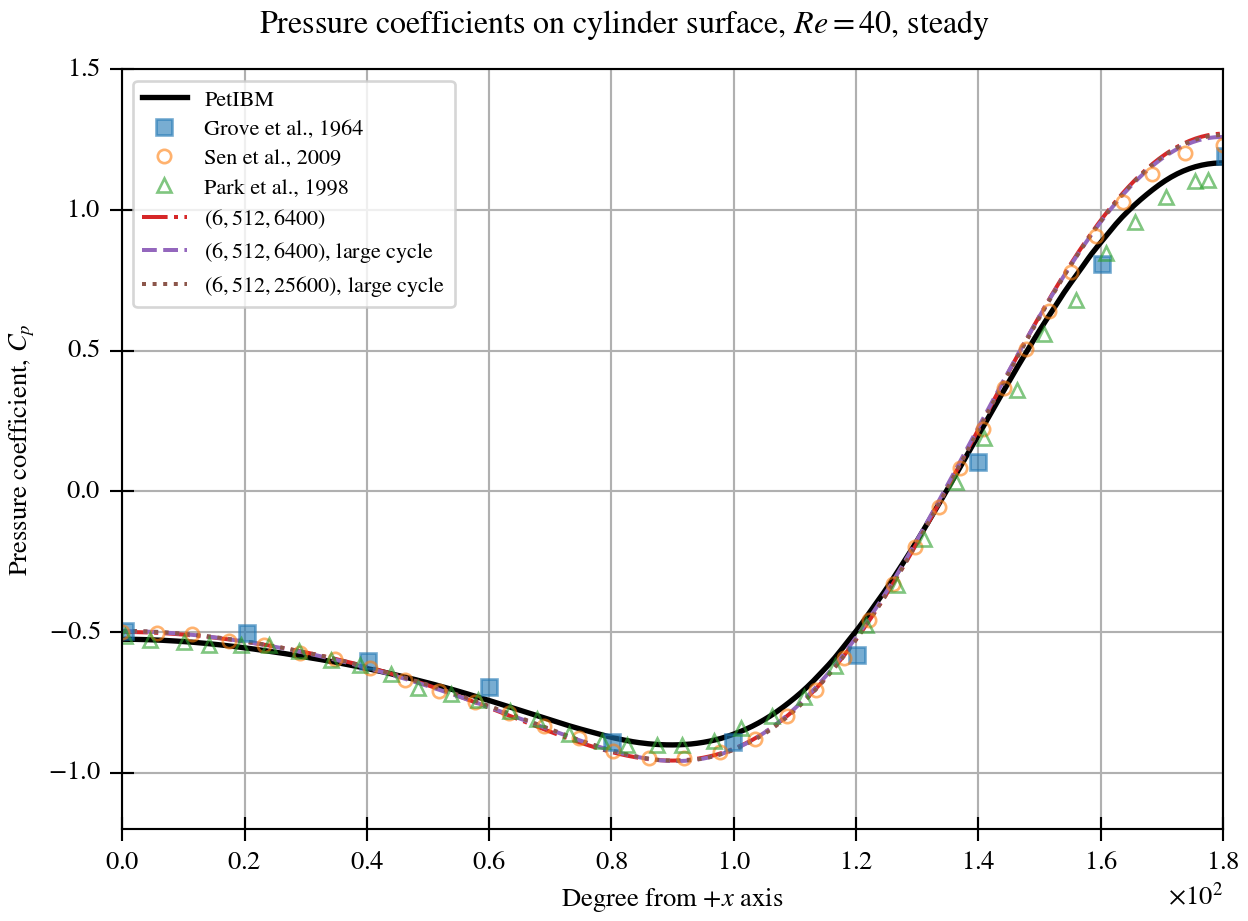
\includegraphics[width=0.9\linewidth]{cylinder-2d-re40/surface-pressure-steady}
    \caption[
        PINNs, 2D Cylinder, $Re=40$: pressure coefficients on cylinder surface for steady solvers%
    ]{
        PINNs, 2D Cylinder, $Re=40$: pressure coefficients on cylinder surface for steady solvers%
        The data from Grove et al., 1964 are experimental, while others are computational.
    }%
    \label{fig:cylinder-2d-re40-surface-cp-steady}
\end{figure}
\begin{figure}[hbt!]
    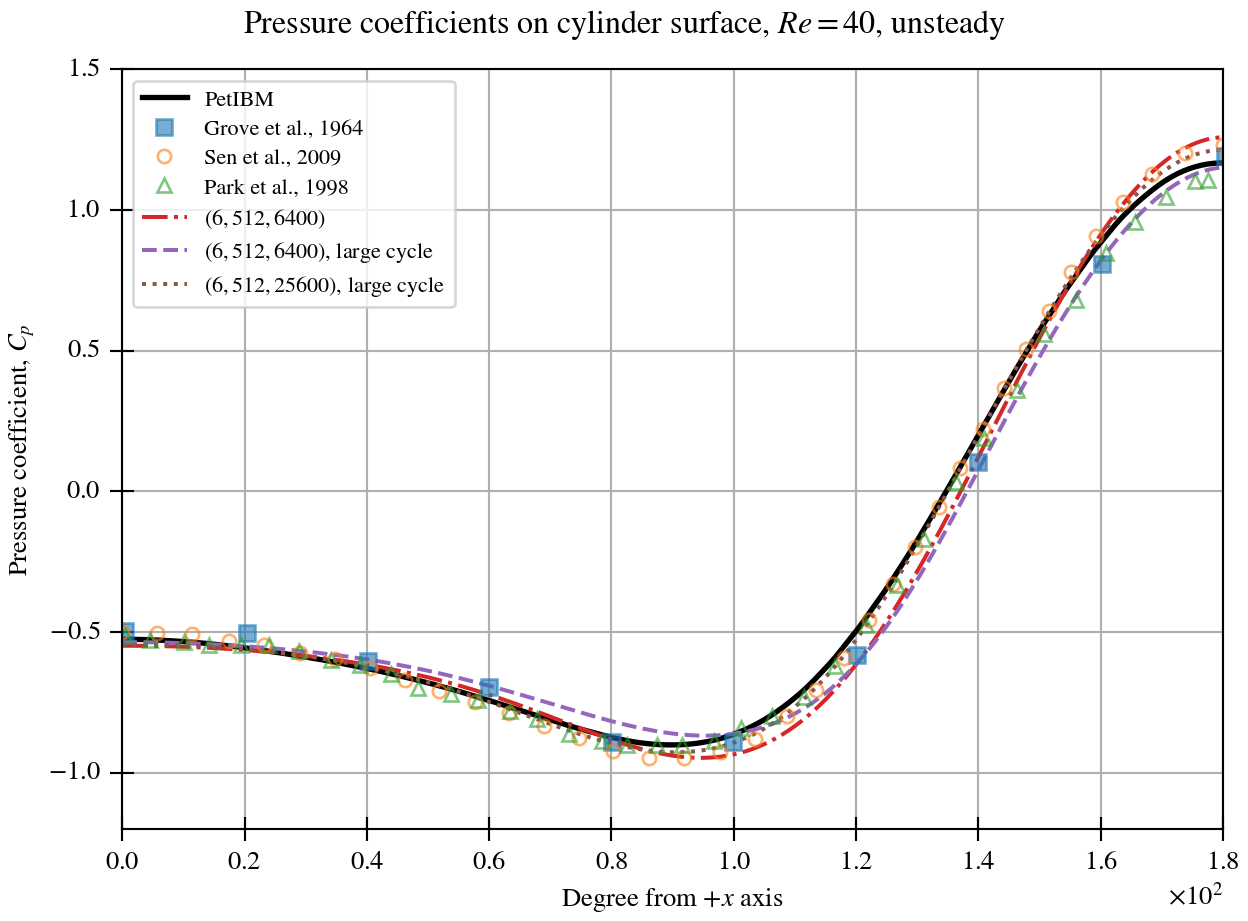
\includegraphics[width=0.9\linewidth]{cylinder-2d-re40/surface-pressure-unsteady}
    \caption[
        PINNs, 2D Cylinder, $Re=40$: pressure coefficients on cylinder surface for unsteady solvers%
    ]{
        PINNs, 2D Cylinder, $Re=40$: pressure coefficients on cylinder surface for unsteady solvers%
        The data from Grove et al., 1964 are experimental, while others are computational.
    }%
    \label{fig:cylinder-2d-re40-surface-cp-unsteady}
\end{figure}
As there is no correct answer, we consider the results of the surface $C_p$ validated.
All results from PINNs are visually within the range made up by the reference data.
% vim:ft=tex

\section{Unsteady 2D Cylinder Flow: Vortex Shedding at \texorpdfstring{$Re=200$}{re200}}
\label{sec:pinn-2d-cylinder-re200}

    \subsection{Problem Description and Configurations}
    \label{sec:pinn-2d-cylinder-re200-conf}
    %! TEX root = main.tex
With the successful validation for the $Re=40$ cylinder flow, we now would like to test an unsteady cylinder flow at $Re=200$.

The computational spatial domain is $[-8$, $25]$ $\times$ $[-8$, $8]$, and the simulation time range is $t\in[0$, $200]$.
Other problem setups are the same as those in section \ref{sec:pinn-2d-cylinder-re40-conf}, except for the kinematic viscosity.
The non-dimensional kinematic viscosity is $0.005$ to make the Reynolds number $200$.

The network architecture is the same: $(N_l$, $N_n)$ $=$ $(6$, $512)$.
We also used a steady and an unsteady PINN solver on this problem, though $Re=200$ is not expected to have a steady-state solution.
The batch size and the configurations of training points are the same as the case of $N_{bs}=\num{6400}$ in section \ref{sec:pinn-2d-cylinder-re40-conf}.
We only used one cyclical learning rate schedule: $(\eta_{low}$, $\eta_{high}$, $N_c$, $\gamma)$ $=$ $(\num{1e-6}$, $\num{1e-2}$, $5000$, $0.9999915)$.

In addition to the steady and unsteady PINN solvers, a third case was done in this benchmark.
This case is a data-driven PINN simulation.
In this data-driven PINN case, we removed the original IC and train the PINN model against several snapshots from a PetIBM simulation.
The selected snapshots from PetIBM were those at $t=125$, $126$, $\cdots$, $139$, $140$.
These snapshots contain around $3$ full periods of vortex shedding.
In other words, we replaced the IC loss terms in equation \eqref{eq:total-residual} with  
\begin{equation}\label{eq:data-driven-loss}
    \left\{
        \begin{aligned}
            &r_{data,\vec{u}}(\Theta) = \sum\limits_{i=1}^{N_{data}}\lVert G_i^{\vec{u}} - \vec{u}_{data, i}\rVert^2 \\
            &r_{data,p}(\Theta) = \sum\limits_{i=1}^{N_{data}}\left( G_i^{p} - p_{data, i} \right)^2
        \end{aligned}
    \right.
\end{equation}
where subscript $data$ denotes the data from the PetIBM simulation.
The total number of data points from PetIBM is around $\num{17000000}$, and we only used $\num{6400}$ every iteration, meaning each data batch was repeated approximately every $\num{2650}$ iterations.
Except for replacing the IC losses with a data-driven approach, all other loss terms in \eqref{eq:total-residual} remain the same.

Note that for the data-driven case, the loss terms of PDEs and BCs were evaluated only in $t\in[125$, $200]$ because we treated PetIBM's data as if they were ICs.
Also, because PDEs were solved even after $t=140$ (the last snapshot from PetIBM), we expected this trained model to be able to make predictions for $t>140$.

Each case ran for $\num{1000000}$ iterations with the Adam optimizer.
The hardware used was 1 NVIDIA A100 GPU for all cases.

The mentioned PetIBM simulation was done on the same K40 configuration as described in section \ref{sec:pinn-2d-cylinder-re40-conf}.
The solver configuration is the same as well, except that the grid resolution is $1485$ $\times$ $720$.
% vim:ft=tex


    \subsection{Results}
    \label{sec:pinn-2d-cylinder-re200-results}
    %! TEX root = main.tex
The overall run times for the steady, unsteady, and data-driven cases are about 28 hours, 31 hours, and 33.5 hours.
The PetIBM simulation, on the other hand, took around 1.7 hours with a 5-generation-behind GPU.

Figure \ref{fig:cylinder-re200-train-hist} shows the convergence history of all cases.
\begin{figure}[hbt!]
    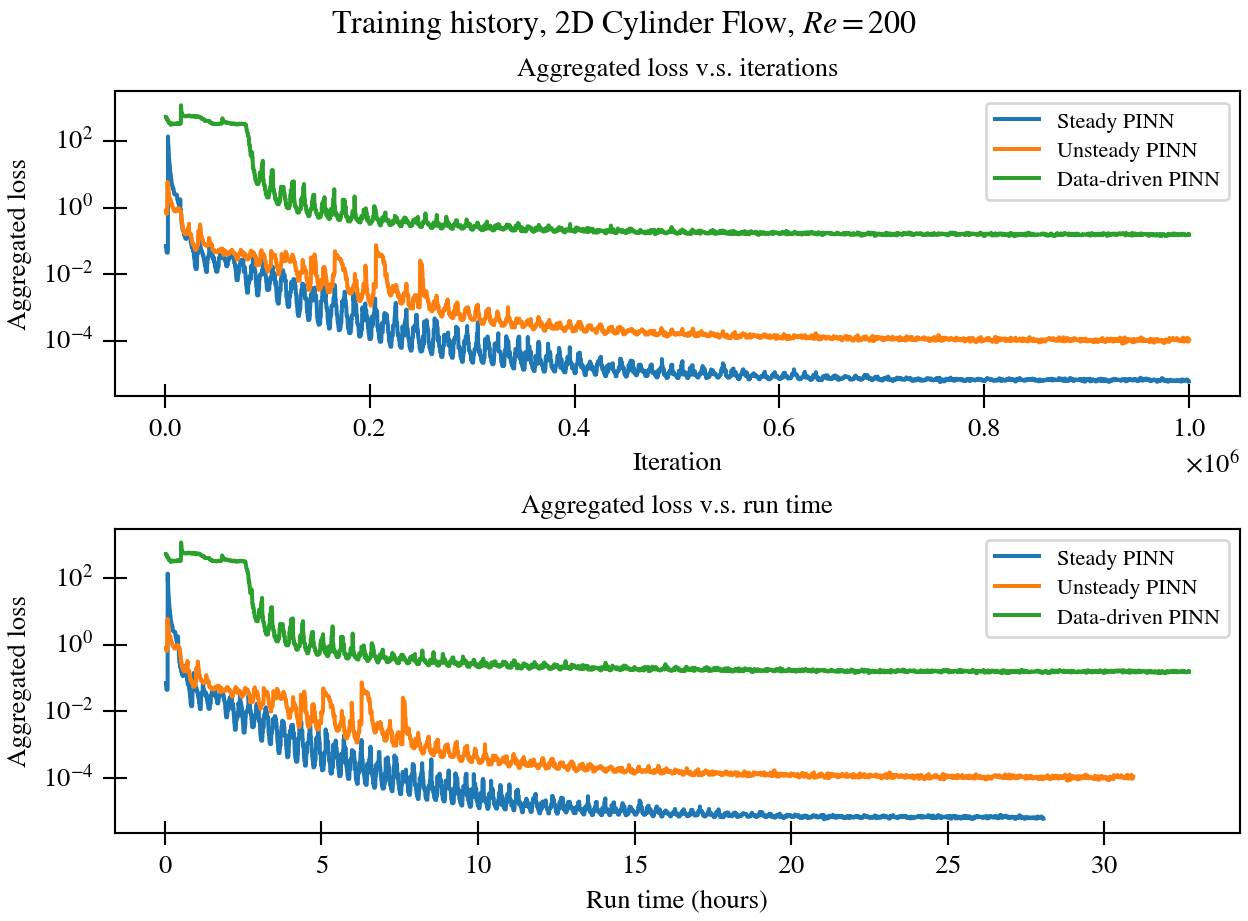
\includegraphics[width=0.9\linewidth]{cylinder-2d-re200/loss-hist}
    \caption{PINNs, 2D Cylinder, $Re=200$: training history}
    \label{fig:cylinder-re200-train-hist}
\end{figure}
One sub-plot is for losses versus iterations, while the other one is against the run times.
The plateaus we observed in the $Re=40$ cases also exist in the unsteady and data-driven cases here.
The steady case does not show any sign of the plateau.
The data-driven case does not converge to a loss level as small as that of the other two cases.
However, the aggregated loss of the data-driven case has extra data loss terms, so it is unclear at this point if all loss terms have higher values or only the data loss terms are higher. 

\begin{table}[hbt!]
    \singlespacing
    \begin{threeparttable}[b]
        \begin{tabular}{lcc}
            \toprule
            & $C_D$ \\
            \midrule
            PetIBM & 1.38   \\
            Steady PINN & 0.95 \\
            Unsteady PINN & 0.95 \\
            Deng et al., 2007\cite{deng_hydrodynamic_2007}\tnote{1} & 1.25 \\
            Rajani et al., 2009\cite{Rajani2009}\tnote{1} & 1.34 \\
            Gushchin \& Shchennikov, 1974\cite{gushchin_numerical_1974}\tnote{2} & 0.97 \\
            Fornberg, 1980\cite{fornberg_numerical_1980}\tnote{2} & 0.83 \\
            \bottomrule
        \end{tabular}%
        \begin{tablenotes}
            \footnotesize
            \item [1] Unsteady simulations.
            \item [2] Steady simulations.
        \end{tablenotes}
        \caption[
            PINNs, 2D Cylinder, $Re=200$: validation of drag coefficients%
        ]{%
            PINNs, 2D Cylinder, $Re=200$: validation of drag coefficients.%
            The data-driven case is excluded because it does not have an obvious periodic state nor a steady-state solution.%
        }%
        \label{table:cylinder-2d-re200-cd}
    \end{threeparttable}
\end{table}%


\begin{figure}[hbt!]
    \includegraphics[width=0.9\linewidth]{cylinder-2d-re200/drag-lift-coeffs}
    \caption{PINNs, 2D Cylinder, $Re=200$: drag and lift coefficients}
    \label{fig:cylinder-re200-drag-lift}
\end{figure}

Figure \ref{fig:cylinder-re200-drag-lift} shows the drag and lift coefficients versus simulation time.
The coefficients from the steady case is just a horizontal line because there is no time variable in this case.
The unsteady case, to our surprise, does not exhibit oscillation, meaning probably no vortex shedding.
Although, it fits well with the PetIBM result before shedding happens (before around $t=75$), including the wake development stage before $t=25$.
Comparing the coefficients between the steady, unsteady, and PetIBM's values before shedding, we believe the unsteady PINN in this particular case behaves just like a steady solver.
This speculation is further supported by the values in table \ref{table:cylinder-2d-re200-cd}, where we compare $C_D$ to both unsteady and steady numerical simulations from literature.
The $C_D$ obtained from the unsteady PINN is the same as the steady PINN and close to those steady CFD simulation results.

As for the data-driven case, its temporal domain is $t\in[125$, $200]$, so the coefficients' trajectories start from $t=125$.
The result, again unexpected to us, only exhibits shedding in the time range where we provide data with shedding to the PINN ($t\in[125$, $140]$).
This result also shows that data-driven PINNs may be more difficult to train, compared to data-free PINNs and regular data-only model fitting.
Even in the range of provided data, the data-driven case is not able to reach the given maximal $C_L$, and the $C_D$ is obviously off from the given data.
After $t=140$, the trajectories quickly fall back to the no-shedding pattern, though it still deviates from the trajectories of the steady and unsteady PINNs.
Combining the loss magnitude shown in figure \ref{fig:cylinder-re200-train-hist}, the deviation of values may be caused by not enough training.
As figure \ref{fig:cylinder-re200-train-hist} shows data-driven PINN is converged, other optimization techniques or hyperparameter tuning may be required to further reduce the loss.

Nevertheless, we believe not being trained enough only explains why the data-driven case deviates from the given data and the trajectories of the other two cases.
Even with a better optimization and eventually a lower loss, based on the trajectories, we do not believe the shedding will continue after $t=140$.

To examine how the transient flow develops, below we show several snapshots of the flow fields from PetIBM and PINNs:
\begin{enumerate}
    \item Figure \ref{fig:cylinder-re200-contour-steady} shows the flow field obtained from the steady PINN as a reference.
    \item Figures \ref{fig:cylinder-re200-contour-uv-t10} and \ref{fig:cylinder-re200-contour-pwz-t10}: flow at $t=10$. We can see the wake is still developing, and the unsteady PINN visually matches PetIBM. It means the unsteady PINN is indeed an unsteady solver. This time is out of the data-driven PINN's temporal domain.
    \item Figures \ref{fig:cylinder-re200-contour-uv-t50} and \ref{fig:cylinder-re200-contour-pwz-t50}: flow at $t=50$. These figures further confirm that the unsteady PINN matches the PetIBM simulation before shedding.
    \item Figures \ref{fig:cylinder-re200-contour-uv-t140} and \ref{fig:cylinder-re200-contour-pwz-t140}: flow at $t=140$. At this point, the shedding already happened. And $t=140$ is the last snapshot we fed to the data-driven PINN for training. The flow from data-driven PINN shows that it at least is able to qualitatively capture the shedding, which is expected.
    \item Figures \ref{fig:cylinder-re200-contour-uv-t144} and \ref{fig:cylinder-re200-contour-pwz-t144}: flow at $t=144$. Just $4$ unit time from the last snapshot we fed to the data-driven PINN, the data-driven PINN has already stopped generating new vortices. The existing vortex can be seen moving toward the boundary, and the wake is gradually recovering to the steady state wake.
    \item Figures \ref{fig:cylinder-re200-contour-uv-t190} and \ref{fig:cylinder-re200-contour-pwz-t190}: flow at $t=190$. Flow field at this time further confirms that the data-driven PINN's behavior is leaning toward that of the unsteady PINN, which is itself behaving like a steady state solver.
\end{enumerate}

\begin{figure}[hbt!]
    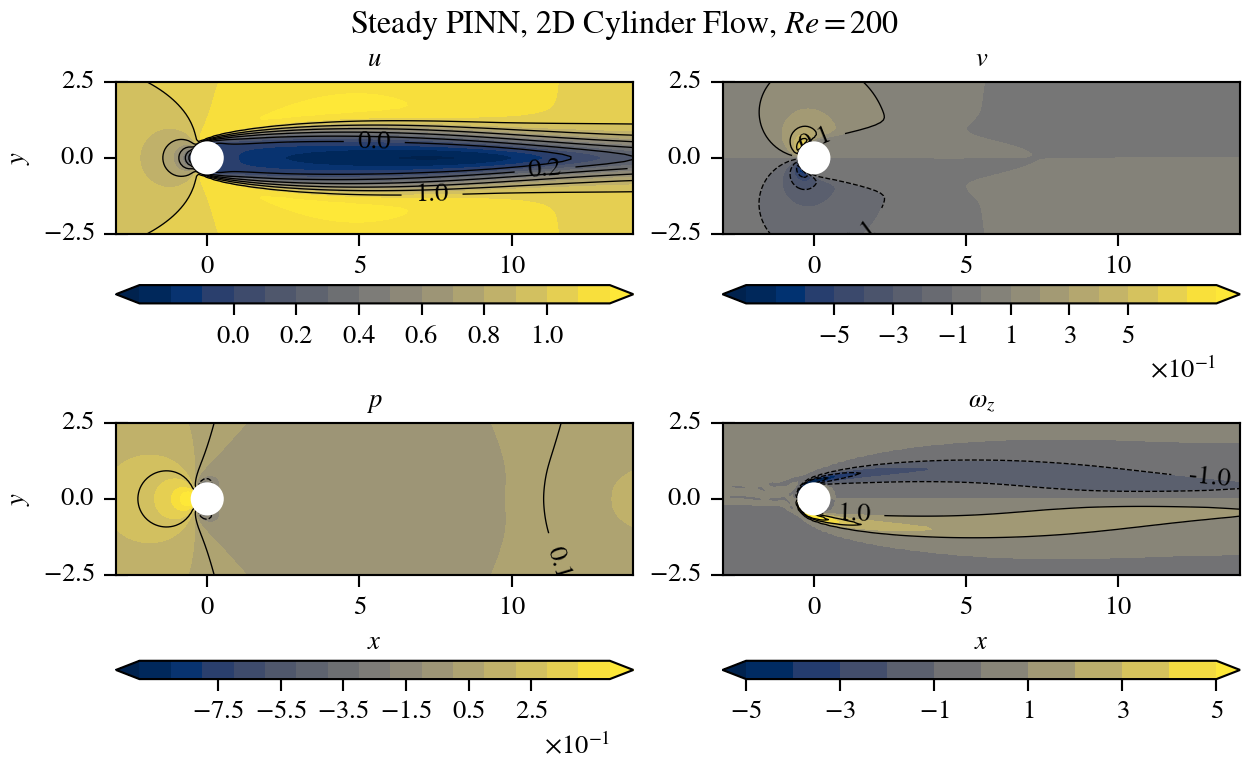
\includegraphics[width=0.9\linewidth]{cylinder-2d-re200/contour-comparison-steady}
    \caption{2D Cylinder, $Re=200$: flow field contours for steady PINN}
    \label{fig:cylinder-re200-contour-steady}
\end{figure}

\begin{figure}[hbt!]
    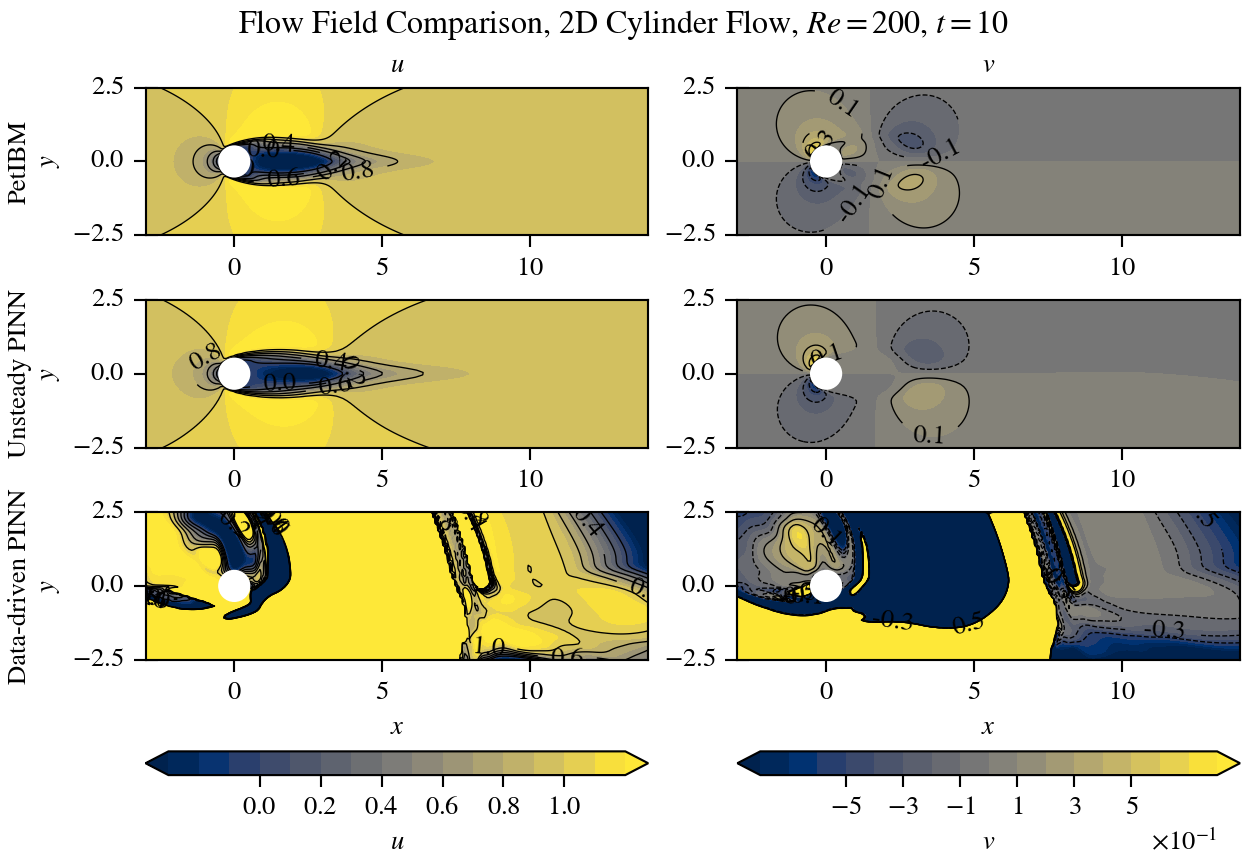
\includegraphics[width=0.9\linewidth]{cylinder-2d-re200/contour-comparison-uv-t10}
    \caption{2D Cylinder, $Re=200$: flow field comparisons for $u$ and $v$ at $t=10$ (PetIBM, data-driven PINN, and data-free PINN)}
    \label{fig:cylinder-re200-contour-uv-t10}
\end{figure}

\begin{figure}[hbt!]
    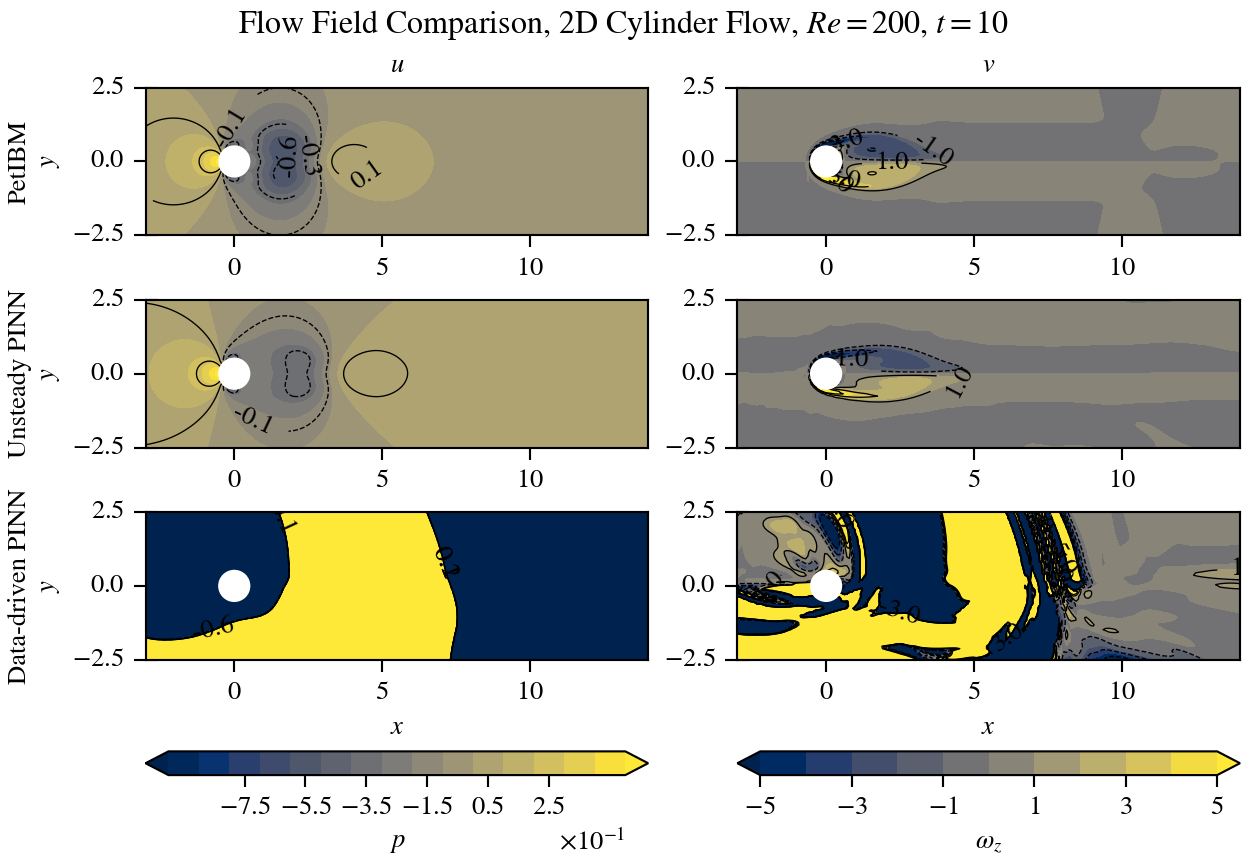
\includegraphics[width=0.9\linewidth]{cylinder-2d-re200/contour-comparison-pwz-t10}
    \caption{2D Cylinder, $Re=200$: flow field comparisons for $p$ and $\omega_z$ at $t=10$ (PetIBM, data-driven PINN, and data-free PINN)}
    \label{fig:cylinder-re200-contour-pwz-t10}
\end{figure}

\begin{figure}[hbt!]
    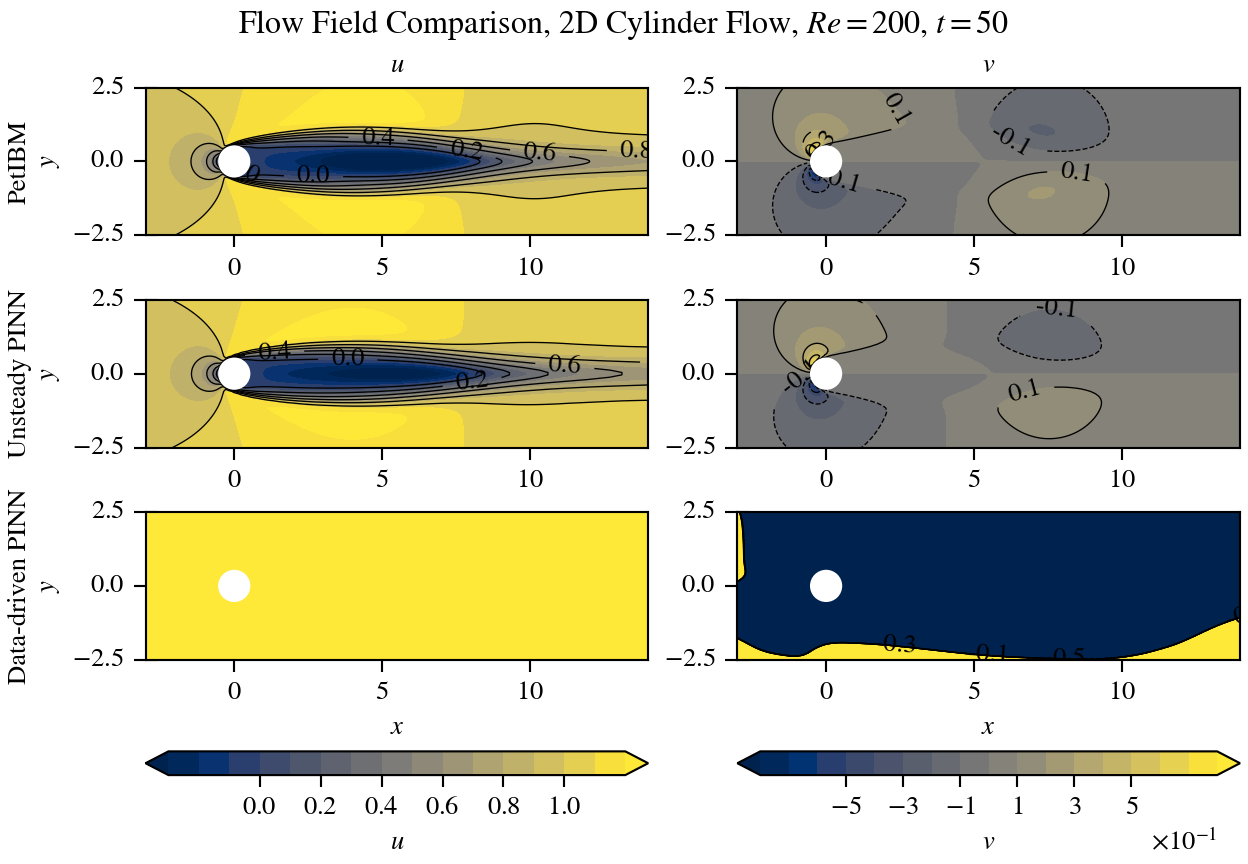
\includegraphics[width=0.9\linewidth]{cylinder-2d-re200/contour-comparison-uv-t50}
    \caption{2D Cylinder, $Re=200$: flow field comparisons for $u$ and $v$ at $t=50$ (PetIBM, data-driven PINN, and data-free PINN)}
    \label{fig:cylinder-re200-contour-uv-t50}
\end{figure}

\begin{figure}[hbt!]
    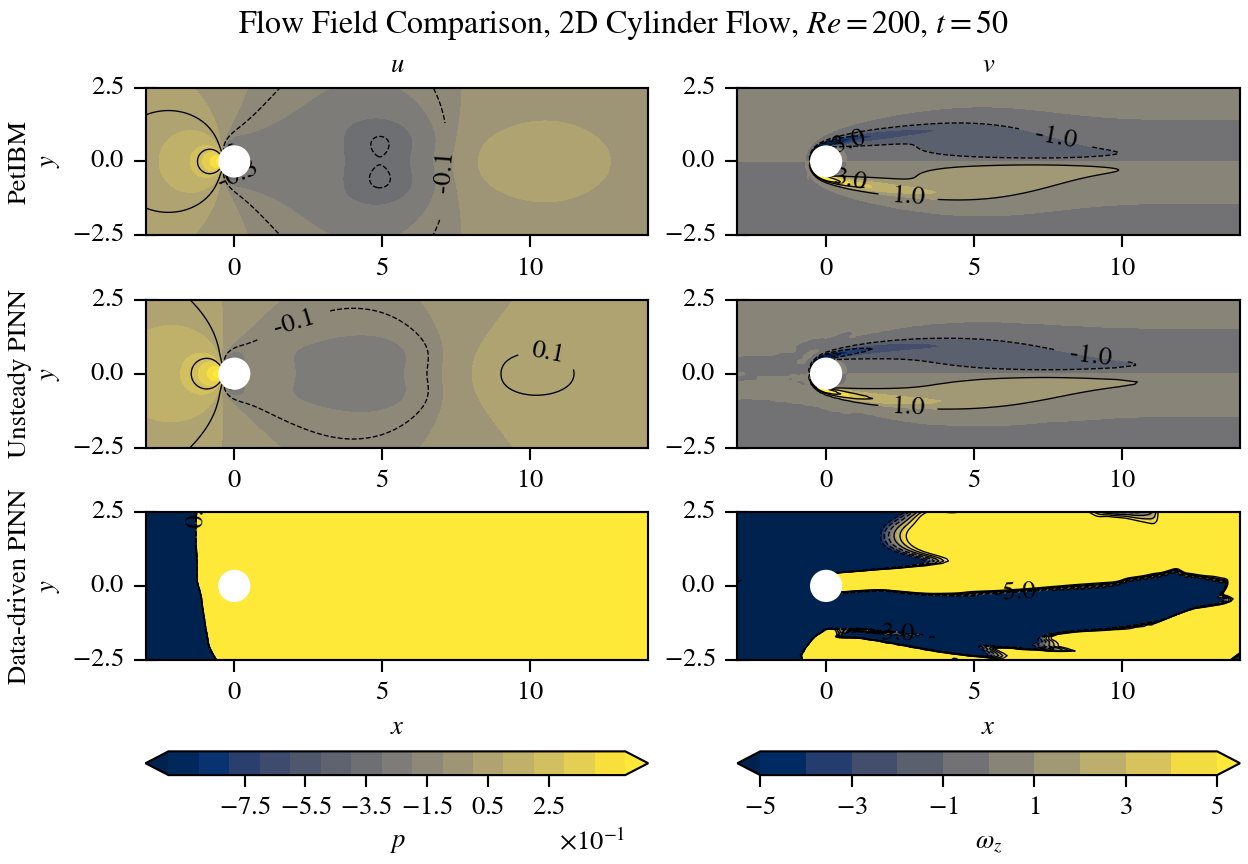
\includegraphics[width=0.9\linewidth]{cylinder-2d-re200/contour-comparison-pwz-t50}
    \caption{2D Cylinder, $Re=200$: flow field comparisons for $p$ and $\omega_z$ at $t=50$ (PetIBM, data-driven PINN, and data-free PINN)}
    \label{fig:cylinder-re200-contour-pwz-t50}
\end{figure}

\begin{figure}[hbt!]
    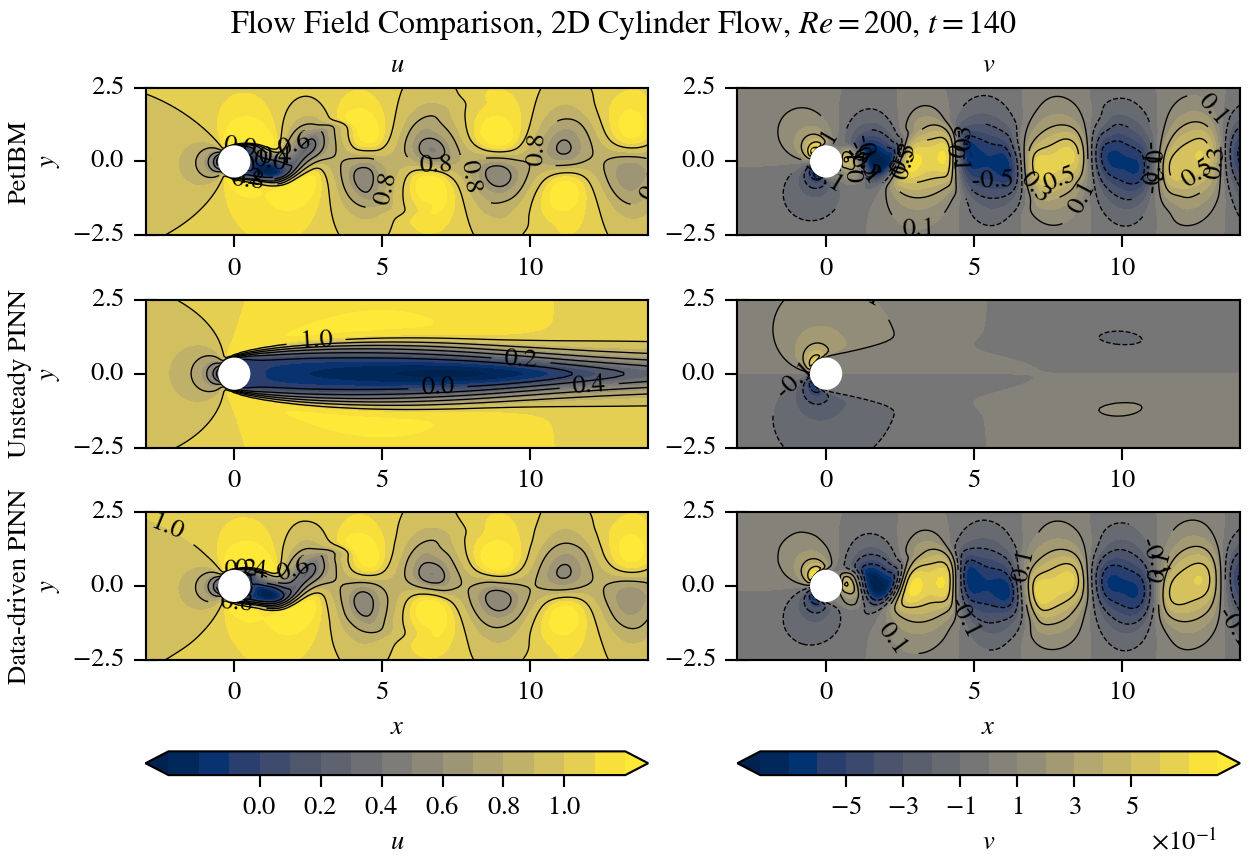
\includegraphics[width=0.9\linewidth]{cylinder-2d-re200/contour-comparison-uv-t140}
    \caption{2D Cylinder, $Re=200$: flow field comparisons for $u$ and $v$ at $t=140$ (PetIBM, data-driven PINN, and data-free PINN)}
    \label{fig:cylinder-re200-contour-uv-t140}
\end{figure}

\begin{figure}[hbt!]
    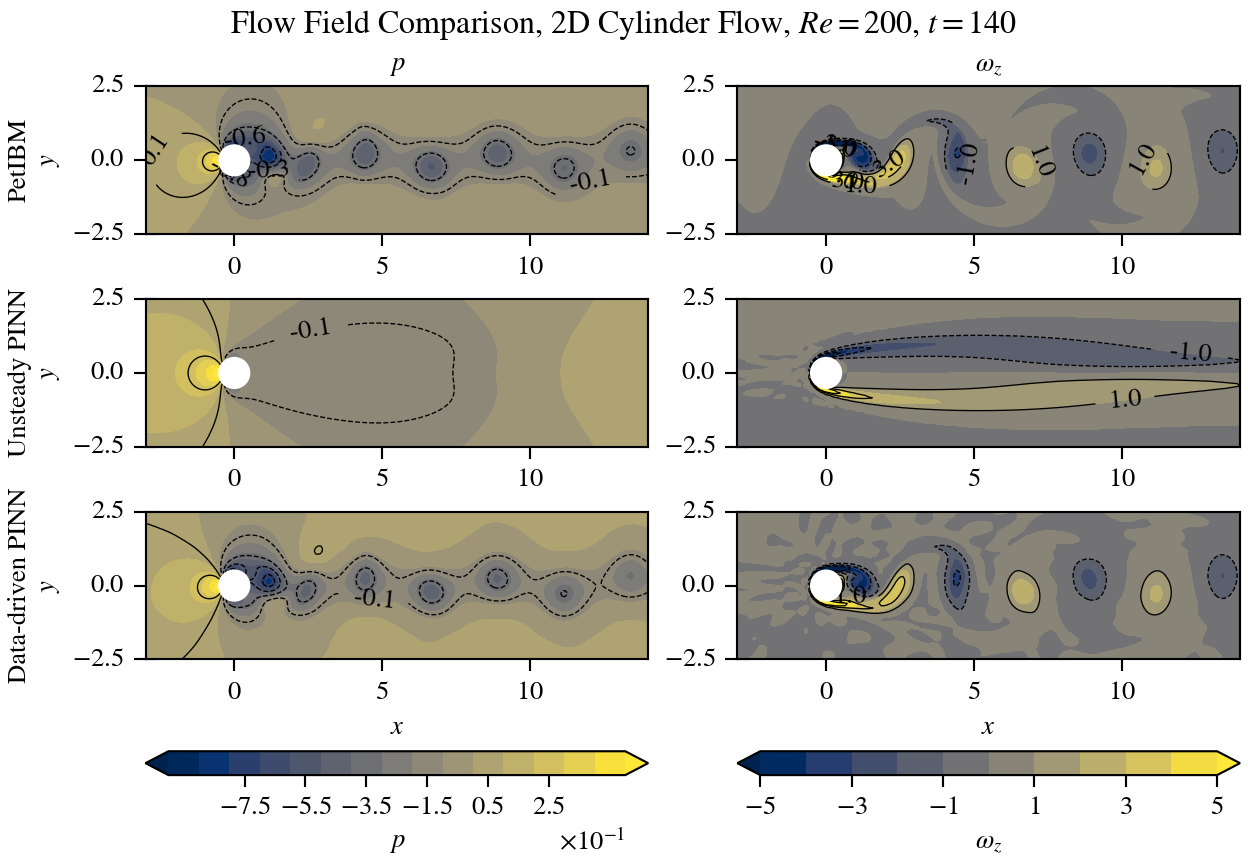
\includegraphics[width=0.9\linewidth]{cylinder-2d-re200/contour-comparison-pwz-t140}
    \caption{2D Cylinder, $Re=200$: flow field comparisons for $p$ and $\omega_z$ at $t=140$ (PetIBM, data-driven PINN, and data-free PINN)}
    \label{fig:cylinder-re200-contour-pwz-t140}
\end{figure}

\begin{figure}[hbt!]
    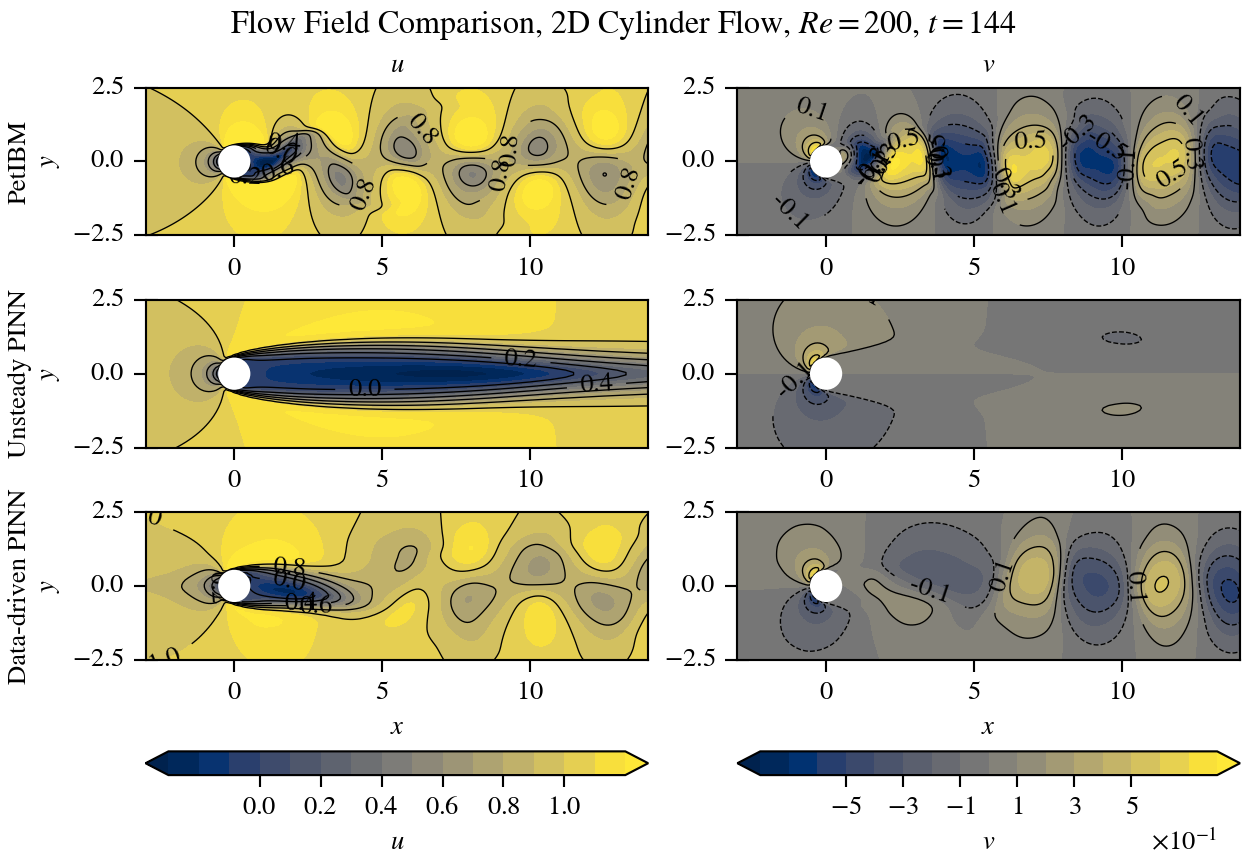
\includegraphics[width=0.9\linewidth]{cylinder-2d-re200/contour-comparison-uv-t144}
    \caption{2D Cylinder, $Re=200$: flow field comparisons for $u$ and $v$ at $t=144$ (PetIBM, data-driven PINN, and data-free PINN)}
    \label{fig:cylinder-re200-contour-uv-t144}
\end{figure}

\begin{figure}[hbt!]
    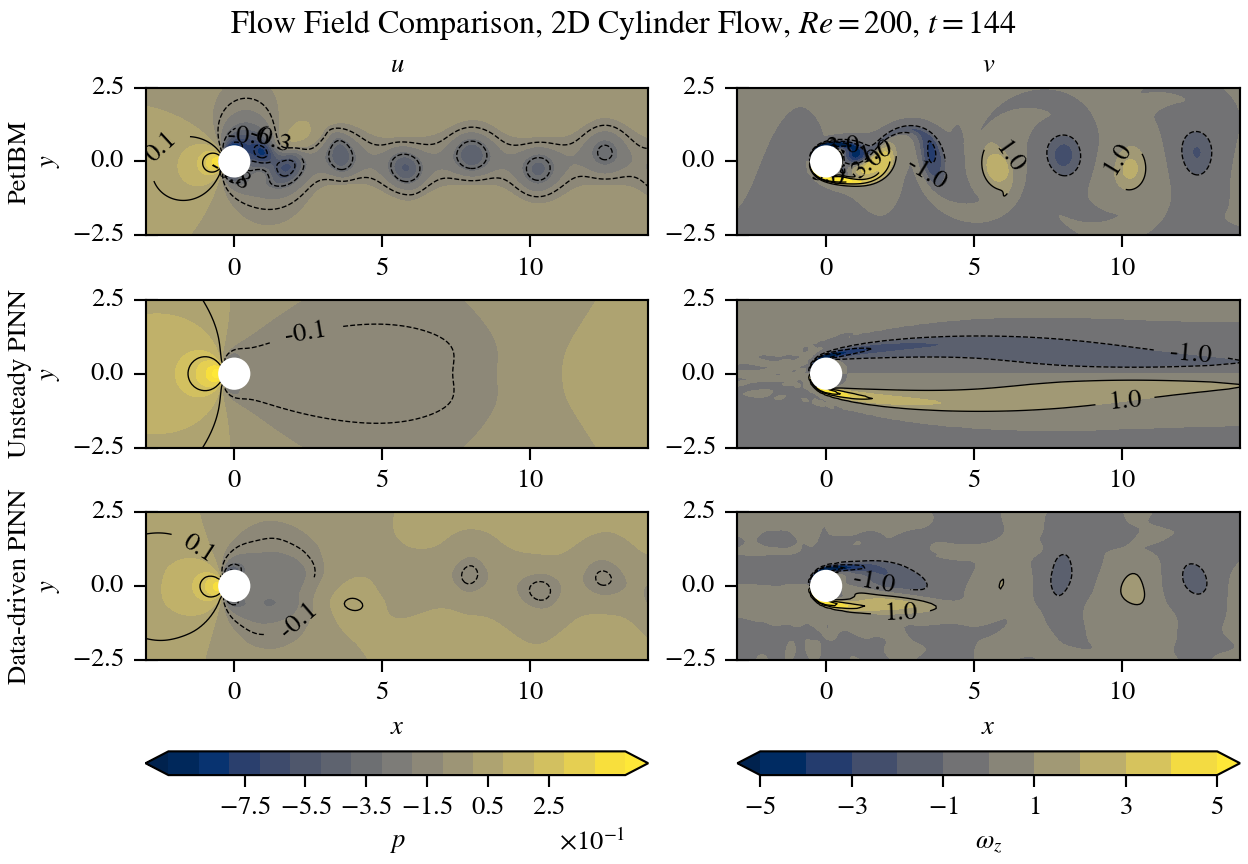
\includegraphics[width=0.9\linewidth]{cylinder-2d-re200/contour-comparison-pwz-t144}
    \caption{2D Cylinder, $Re=200$: flow field comparisons for $p$ and $\omega_z$ at $t=144$ (PetIBM, data-driven PINN, and data-free PINN)}
    \label{fig:cylinder-re200-contour-pwz-t144}
\end{figure}

\begin{figure}[hbt!]
    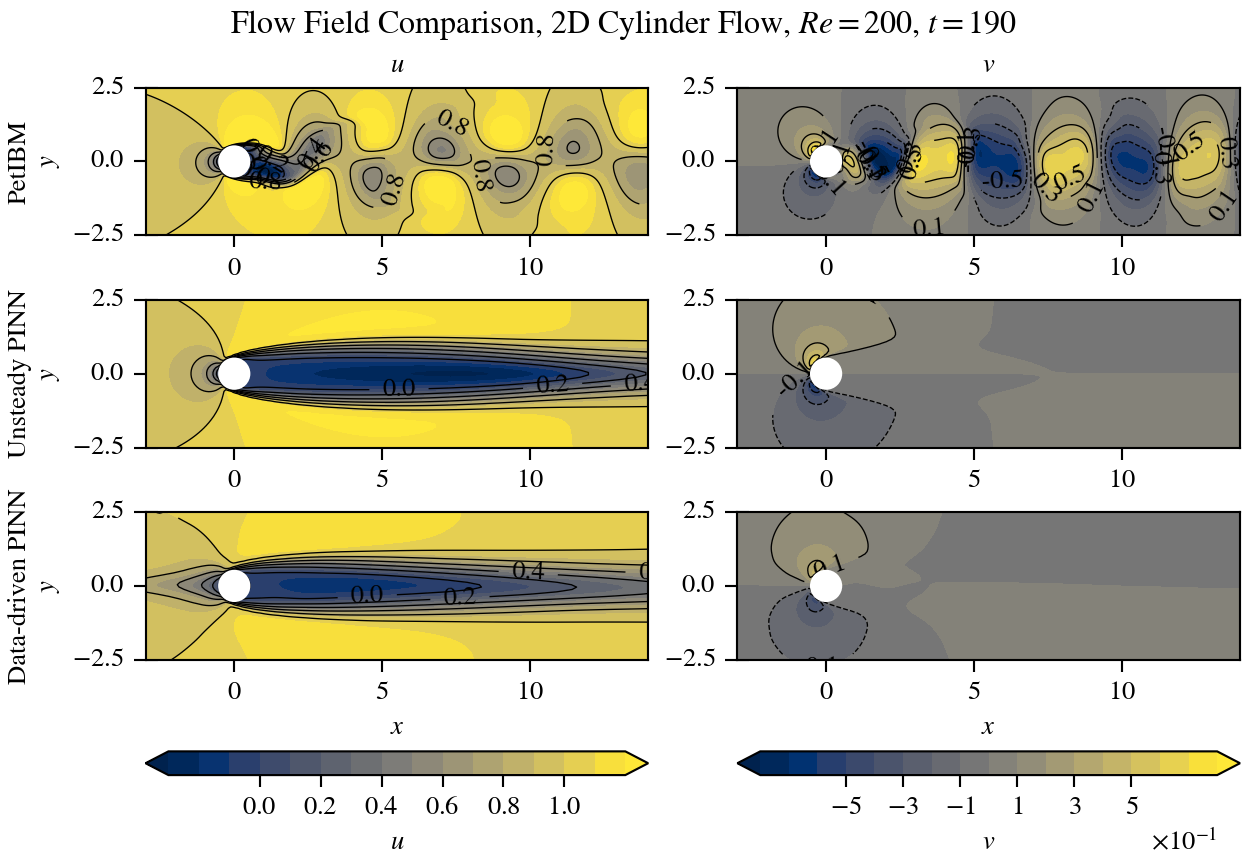
\includegraphics[width=0.9\linewidth]{cylinder-2d-re200/contour-comparison-uv-t190}
    \caption{2D Cylinder, $Re=200$: flow field comparisons for $u$ and $v$ at $t=190$ (PetIBM, data-driven PINN, and data-free PINN)}
    \label{fig:cylinder-re200-contour-uv-t190}
\end{figure}

\begin{figure}[hbt!]
    \includegraphics[width=0.9\linewidth]{cylinder-2d-re200/contour-comparison-pwz-t190}
    \caption{2D Cylinder, $Re=200$: flow field comparisons for $p$ and $\omega_z$ at $t=190$ (PetIBM, data-driven PINN, and data-free PINN)}
    \label{fig:cylinder-re200-contour-pwz-t190}
\end{figure}

\clearpage

Figures \ref{fig:cylinder-2d-re200-refined-vort-1} and \ref{fig:cylinder-2d-re200-refined-vort-2} show the vorticity from PetIBM and the data-driven PINN in the vicinity of the cylinder in $t \in [140, 142.5]$, which contains a half cycle of vortex shedding.
These figures compare how vorticity was generated right after we stopped feeding PetIBM data into the data-driven PINN.
These comparisons were expected to shed some light on why the data-free PINN was not able to generate vortex shedding and why the vortex shedding disappeared in the data-driven PINN after $t=140$.

At $t=140$, PetIBM and the data-driven PINN show visually indistinguishable vorticity contours.
This is expected as the data-driven PINN has training data from PetIBM at this time.
At $t=140.5$, a slight difference exists in the result, though nothing seems unphysical.

At $t=141$ and $141.5$ and in PetIBM's results, the main clockwise vortex (the blue circular pattern in the domain of $[1, 2]\times[-0.5, 0.5]$) moves downstream, and it slows down the downstream's $u$ velocity and accelerates the latter's $v$ velocity in $y<0$.
Intuitively, we can treat the main clockwise vortex as a blocker that blocks the flow in $y<0$ and forces the flow move upward.
The net effect is the generation of a counterclockwise vortex at around $x\approx 1$ and $y \in [-0.5, 0]$.
This new counterclockwise vortex further generates a small but strong secondary clockwise vortex on the cylinder surface in $y\in[-0.5, 0]$.
On the other hand, the results of the data-driven PINN at $t=141$ and $t=141.5$ show that the main clockwise vortex becomes more dissipative and weaker, compared to that in PetIBM.
It is possible that the main clockwise vortex is not strong enough to slow down the flow in $y<0$ nor to bring the flow upward.
The downstream flow in $y<0$ (the red arm-like pattern below the cylinder) thus does not change its direction and keeps going straight down in the $x$ direction.

In the results of $t=142$ and $t=142.5$ from PetIBM, the flow completes a half cycle.
That is, the flow pattern at $t=142.5$ is an upside down version of that at $t=140$.
The results from the PINN, however, do not have any new vortices and becomes more like the steady-state flow. 

\begin{figure}[hbt!]
    \centering
    \includegraphics[width=0.925\linewidth]{cylinder-2d-re200/refined/vorticity_z_t140.0}
    \newline
    \includegraphics[width=0.925\linewidth]{cylinder-2d-re200/refined/vorticity_z_t140.5}
    \newline
    \includegraphics[width=0.925\linewidth]{cylinder-2d-re200/refined/vorticity_z_t141.0}
    \caption{2D Cylinder, $Re=200$: vorticity generation comparison in the vicinity of the cylinder; $t=140$, $140.5$, and $141$ (PetIBM and data-driven PINN)}
    \label{fig:cylinder-2d-re200-refined-vort-1}
\end{figure}

\begin{figure}[hbt!]
    \centering
    \includegraphics[width=0.925\linewidth]{cylinder-2d-re200/refined/vorticity_z_t141.5}
    \newline
    \includegraphics[width=0.925\linewidth]{cylinder-2d-re200/refined/vorticity_z_t142.0}
    \newline
    \includegraphics[width=0.925\linewidth]{cylinder-2d-re200/refined/vorticity_z_t142.5}
    \caption{2D Cylinder, $Re=200$: vorticity generation comparison in the vicinity of the cylinder; $t=141.5$, $142$, and $142.5$ (PetIBM and data-driven PINN)}
    \label{fig:cylinder-2d-re200-refined-vort-2}
\end{figure}

Next, we examined the Q-criterion in the same vicinity of the cylinder in $t\in[140, 142.5]$.
Q-criterion is defined as \cite{jeong_identification_1995}:
\begin{equation}
    Q \equiv \frac{1}{2}\left(\lVert \Omega \rVert^2 - \lVert S \rVert^2\right)
\end{equation}
where $\Omega\equiv\frac{1}{2}\left(\nabla\vec{u}-\nabla\vec{u}^\mathsf{T}\right)$ is the vorticity tensor (i.e., rotation rate tensor); $S\equiv\frac{1}{2}\left(\nabla\vec{u}+\nabla\vec{u}^\mathsf{T}\right)$ is the strain rate tensor; and $\nabla\vec{u}$ is the velocity gradient tensor.
A criterion $Q > 0$ identifies the vortex structure in fluid flow, that is, where the rotation rate is greater than the strain rate.
Figures \ref{fig:cylinder-2d-re200-refined-q-1} and \ref{fig:cylinder-2d-re200-refined-q-2} show the Q-criterion results.
We observed that vortices in the PINN are diffusive and could be dissipative.
Moreover, judging by the locations of vortex centers, vortices also move slower in the PINN than in PetIBM.
The edges of the vortices move at a different speed from that of the vortex centers in the PINN.
This might be hinting the existence of the numerical dispersion in the PINN.

\begin{figure}[hbt!]
    \centering
    \includegraphics[width=0.925\linewidth]{cylinder-2d-re200/refined/qcriterion_t140.0}
    \newline
    \includegraphics[width=0.925\linewidth]{cylinder-2d-re200/refined/qcriterion_t140.5}
    \newline
    \includegraphics[width=0.925\linewidth]{cylinder-2d-re200/refined/qcriterion_t141.0}
    \caption{2D Cylinder, $Re=200$: Q-criterion in the vicinity of the cylinder; $t=140$, $140.5$, and $141$ (PetIBM and data-driven PINN)}
    \label{fig:cylinder-2d-re200-refined-q-1}
\end{figure}

\begin{figure}[hbt!]
    \centering
    \includegraphics[width=0.925\linewidth]{cylinder-2d-re200/refined/qcriterion_t141.5}
    \newline
    \includegraphics[width=0.925\linewidth]{cylinder-2d-re200/refined/qcriterion_t142.0}
    \newline
    \includegraphics[width=0.925\linewidth]{cylinder-2d-re200/refined/qcriterion_t142.5}
    \caption{2D Cylinder, $Re=200$: Q-criterion in the vicinity of the cylinder; $t=141.5$, $142$, and $142.5$ (PetIBM and data-driven PINN)}
    \label{fig:cylinder-2d-re200-refined-q-2}
\end{figure}

In the next subsection, we would like to apply the spectral analysis to further investigate how information propagate in the temporal direction in the PINN.

\FloatBarrier
% vim:ft=tex


    \subsection{Spectral and Koopman Analysis}
    \label{sec:pinn-2d-cylinder-re200-koopman}
    %! TEX root = main.tex

In this subsection, we conducted spectral analysis on the cylinder flow to extract frequencies embedded in the simulation results.
Fluid flow is a dynamical system, and how information (or signals) propagates in time plays an important role.
Information with different frequencies advances at different speeds in the temporal direction, and the superposition of information forms complicated flow patterns over time.
Spectral analysis reveals frequencies and corresponding information---which is called {\it dynamic modes} in fluid dynamics.
By comparing the spectral results against PetIBM, we examined how well/badly the data-driven PINN learned information with different frequencies.

We used Koopman analysis \cite{chen_variants_2012,rowley_spectral_2009} to generate the spectral results.
When having time-series solutions of a dynamical system but not knowing the exact propagation mechanism in the temporal direction, Koopman analysis helps identify the system's characteristics, including frequencies and complex-valued dynamic modes.
Here we skip the details of the Koopman analysis.
Please refer to {\it the method of snapshots} in reference \cite{chen_variants_2012} for the theory and the algorithms we used.

Given $m+1$ flow snapshots with a uniform time spacing $\Delta t$: $\vec{g}_0$, $\vec{g}_1$, $\dots$, $\vec{g}_m \in \mathbb{R}^{N}$, our goal is to express these solutions as the superpositions of $m$ dynamic modes:
\begin{equation}\label{eq:discrete-dmd}
    \vec{g}_k
    =
    \sum\limits_{j=1}^{m}
    \vec{v}_j
    \exp\left(\left( \alpha_j + 2 \pi f_j i\right) k \Delta t\right)
    ,\quad
    k = 0, 1, \cdots, m
\end{equation}
which is a discretized version of the following continuous complex-valued series expansion:
\begin{equation}\label{eq:continuous-dmd}
    \vec{g}(\vec{x}, t)
    =
    \sum\limits_{j=1}^{m}
    \vec{v}_j(\vec{x})
    \exp\left(\left( \alpha_j + 2\pi f_j i\right) t\right)
\end{equation}
$\vec{v}_j \in \mathbb{C}^{N}$ denotes the $j$-th dynamic mode.
$\alpha_j \in \mathbb{R}$ is called the growth rate because $\exp\left(\alpha_j t\right)$ controls the damping/growth of the $j$-th mode over time.
$f_j \in \mathbb{R}$ is the frequency associated with the $j$-th mode. 
$i$ is the imaginary unit.
Note that for a periodic flow pattern (such as vortex shedding), the growth rate $\alpha_j$ must be zero because no mode can become stronger or weaker.

After applying the Koopman analysis, the outcome provides the following series expansion of the solutions:
\begin{equation}\label{eq:koopman}
    \vec{g}_k
    =
    \sum\limits_{j=1}^{m}
    \lambda_j^k \vec{v}_j
    ,\quad
    k = 0, 1, \cdots, m
\end{equation}
where $\lambda_j \in \mathbb{C}$ is called $j$-th Koopman eigenvalue, and $\lambda_j^k$ is $\lambda_j$ to the power of $k$.
$\vec{v}_j$ is the $j$-th Koopman eigenvector and is the same as the $j$-th dynamic mode in equation \eqref{eq:discrete-dmd}.
Equating equation \eqref{eq:discrete-dmd} and \eqref{eq:koopman} allows us to calculate the growth rates and frequencies using the Koopman eigenvalues:
\begin{equation}
    \left\{
        \begin{array}{l}
            \alpha_j = \frac{1}{\Delta t} \mathfrak{Re}\left(\ln\left(\lambda_j\right)\right) \\
            f_j = \frac{1}{2\pi\Delta t} \mathfrak{Im}\left(\ln\left(\lambda_j\right)\right) \\
        \end{array}
    \right.
\end{equation} 

We analyzed the results from PetIBM and the data-driven PINN in $t\in[125, 140]$, which contains about three full cycles of vortex shedding.
A total of $76$ solution snapshots were used from each solver.
The time spacing is $\Delta t = 0.2$.
The Koopman analysis would result in $75$ modes.
Since the snapshots cover three full cycles, we would expect only $25$ distinct frequencies and $25$ nontrivial modes---only $25$ out of $76$ snapshots are distinct.
However, this expectation only happens when the data are free from noise and numerical errors and when the number of three periods is exact.
We would see more than $25$ distinct frequencies and modes if the data were not ideal.
In $t \in [125, 140]$, the data-driven PINN was trained against PetIBM's data, so we expected to see similar spectral results between the two solvers.

Figure \ref{fig:koopman-eigval-dist} shows the distributions of the Koopman eigenvalues, $\lambda_j$, on the complex plane.
The color of each dot represents the normalized strength of the corresponding mode, defined as:
\begin{equation}
    \text{normalized strength of the }j\text{-th mode}
    \equiv
    \frac{\lVert \vec{v}_j \rVert \sqrt{m+1}}{\sqrt{\sum\limits_{k=0}^{m}\lVert\vec{g}_k\rVert^2}}
\end{equation}
The star marker denotes the mode with $f_j=0$: a steady or time-independent mode.
This mode usually has much higher strength than others, so we excluded it from the color map and annotated its strength on each figure.
Koopman eigenvalues come as complex conjugate pairs, so the modes are symmetric with respect to the real-number axis. 
A conjugate pair has an opposite sign in $f_j$ but has the same physical frequency (e.g., $\exp(2\pi f_jt)$ and $\exp(2\pi (-f_j)t)$ both propagate at the same frequency physically).

We also plotted a circle with a radius of one on each figure.
As flow has already reached a fully periodic regime, the growth rates $\alpha_j$ should be zero, that is, $\mathfrak{Re}\left(\ln\left(\lambda_j\right)\right) = \ln\left(\lvert \lambda_j \rvert\right) = 0$.
In other words, $\lvert \lambda_j \rvert = 1$, meaning all $\lambda_j$ were expected to fall on this circle on the complex plane.
If a mode falls inside the circle, it has a negative growth rate, and its contribution to the solution diminishes over time.
Similarly, a mode falling outside the circle has positive growth over time.

\begin{figure}[hbt!]
    \centering
    \includegraphics[width=0.975\linewidth]{cylinder-2d-re200/koopman/koopman_eigenvalues_complex}
    \caption{2D Cylinder, $Re=200$: Koopman eigenvalue distribution on the complex plane}
    \label{fig:koopman-eigval-dist}
\end{figure}

On the complex plane, all $\lambda_j$ of PetIBM fall onto the circle or close to the circle (on the left in figure \ref{fig:koopman-eigval-dist}).
Though PetIBM's plot shows $75$---rather than $25$---distinct $\lambda_j$ and modes, modes are evenly clustered into 25 groups.
Each group has three modes, among which one or two modes fall on the circle, while the remaining one(s) falls inside but very close to the circle.
Modes within each group have a similar $\lambda_j$, and the one precisely on the circle has significantly higher strength than other modes (if not all modes in the group are weak).
Due to the numerical errors in PetIBM's solutions, data in a vortex period are similar to but not exactly the same as those in another period.
The strong modes falling precisely on the circle may represent the period-averaged flow patterns and are the $25$ modes we expected in the previous paragraphs. 
The effect of numerical errors was filtered out from these modes.
We call these 25 modes primary modes and all other modes secondary modes.
Secondary modes are mostly weak and may come from the numerical errors in the PetIBM simulation.
The plot shows these secondary modes are slightly dispersive but non-increasing over time, which is reasonable because the numerical schemes in PetIBM are stable.

As for the PINN's result (on the right in figure \ref{fig:koopman-eigval-dist}), the mode distribution is not as structured as in PetIBM.
It is hard to distinguish if all 25 expected modes also exist in this plot.
However, we observed that at least the top 7 primary modes (the steady mode, two purple and 4 orange dots on the circle) also exist in the PINN's plot.
Secondary modes spread out more widely on and inside the circle, compared to the clustered modes in PetIBM.
We believe this means the PINN is more numerically dispersive and noisy.
The frequencies of many of these secondary modes do not exist in PetIBM.
So one possible source of these additional frequencies and modes may be the method of PINN itself.
It could be not-enough training or that the neural network itself inherently is dispersive. 
However, secondary modes on the circle are weak.
We suspect that their contribution to the solution may be trivial.

A more concerning observation is the presence of damped modes (modes that fall inside the circle). 
These modes have negative growth rates and hence are damped over time.
We believe these modes contribute significantly to the solution because their strengths are nontrivial.
The existence of the damped modes also means the PINN's predictions have more significant discrepancies from one vortex period to another vortex period, compared to the PetIBM's simulation.
In addition, the flow pattern in PINN would keep changing after $t=140$.
They may be the culprits causing the PINN's solution to quickly fall back to a non-oscillating solution for $t>140$.
We may consider these errors as numerical dissipation.
However, whether these errors came from not being trained enough or were inherent in the PINN is unclear.

Note that the spectral analysis was done against data in $t\in[125, 140]$.
It does not mean the solutions in $t>140$ also have the same spectral characteristics: the flow system is nonlinear, but the Koopman analysis uses linear approximations \cite{rowley_spectral_2009}.

\begin{figure}[hbt!]
    \centering
    \includegraphics[width=0.975\linewidth]{cylinder-2d-re200/koopman/koopman_mode_strength}
    \caption{2D Cylinder, $Re=200$: Koopman mode strength v.s. Strouhal number}
    \label{fig:koopman-freq-st}
\end{figure}

Figure \ref{fig:koopman-freq-st} shows mode strengths versus mode frequencies.
The plots use nondimensional frequency, i.e., Strouhal number $St\equiv\frac{Df}{U_{inlet}}$, in their horizontal axes. 
In our cylinder flow, $D=U_{inlet} = 1$.
We only plotted modes with $f_j \ge 0$ for a concise visualization.
Note that we use a log scale for the vertical axis.
Plots in this figure also show the same observations in the previous paragraphs: the data-driven PINN is more dispersive and dissipative.

An observation that is now clearer from figure \ref{fig:koopman-freq-st} is the strength distribution.
In PetIBM's plot, strengths decrease exponentially from the steady mode (i.e., $St=0$) to high-frequency modes.
One can deduce a similar conclusion from PetIBM's simulation result.
The vortex shedding is dominated by a single frequency (this frequency is $St\approx 0.2$ because $t\in[125, 140]$ contains three periods).
Therefore, the flow should be dominated by the steady mode and a mode with a frequency close to $St=0.2$.
We can indeed verify this statement from PetIBM's plot in figure \ref{fig:koopman-freq-st}: the primary modes of $St=0$ and $St\approx 0.2$ are much stronger than others.
The strength of the immediately next mode, i.e., $St\approx 0.4$, drops in an order of magnitude. 
Note the use of the logarithm scale.
If we re-plot figure \ref{fig:koopman-freq-st} using a regular scale, only $St=0$ and $St=0.2$ would be visible in the figure.

The strength distribution in the PINN's plot also shows that $St=0$ and $St\approx 0.2$ are strong.
However, they are not the only dominating modes.  
Several other modes also have strengths at around $10^{-1}$.
As discovered in the previous paragraphs, these additional strong modes are damped modes.
We also observed that some damped modes have the same frequencies as primary modes.
For example, the secondary modes at $St=0$ and $St=0.2$ are damped modes, which can be confirmed in figure \ref{fig:koopman-eigval-dist}.
Note that for $St=0$, if a mode is damped, then it is not a steady mode anymore because its magnitude changes with time, though it is still non-oscillating.

\begin{table}[hbt!]
    \singlespacing
    \begin{threeparttable}[b]
        \begin{tabular}{ccccc}
            \toprule
            $St$ & Strength\tnote{1} & Growth Rate & Contours \\
            \midrule
            0     & 0.96 & 1.3e-7  & Figure \ref{fig:koopman-petibm-mode-1}\\
            0.201 & 0.20 & -4.3e-7 & Figure \ref{fig:koopman-petibm-mode-2}\\
            0.403 & 0.04 & 1.7e-6  & Figure \ref{fig:koopman-petibm-mode-3}\\
            0.604 & 0.03 & 2.7e-6  & Figure \ref{fig:koopman-petibm-mode-4}\\
            \bottomrule
        \end{tabular}%
        \begin{tablenotes}
            \footnotesize
            \item [1] Normalized.
        \end{tablenotes}
        \caption{%
            2D Cylinder, $Re=200$: top 4 primary dynamic modes (sorted by strengths) for PetIBM%
        }%
        \label{table:koopman-petibm}
    \end{threeparttable}
\end{table}%

Table \ref{table:koopman-petibm} summarizes the top 4 modes (ranked in their strengths) in PetIBM's spectral result.
For reference, these modes' contours are provided in figure \ref{fig:koopman-petibm-mode-1} to \ref{fig:koopman-petibm-mode-4}.
The dynamic modes are complex-valued, and the contours include both the real and the imaginary parts.
Note the growth rates of these 4 modes are not exactly zero but around $10^{-6}$ and $10^{-7}$.
We were unsure if we could treat them as zero at these orders of magnitude.
If not, and if they do cause the primary modes to be slightly damped or augmented over time, then we believe they also serve a reasonable explanation for the existence of the other 50 non-primary modes in PetIBM---to compensate for the loss or the gain in the primary modes.

Table \ref{table:koopman-pinn-non-damped} lists the PINN's top 4 primary modes. They are the same as those in table \ref{table:koopman-petibm}.
Table \ref{table:koopman-pinn-damped} shows the top 4 damped modes in the PINN's result.
Their contours are also indicated in the tables for readers' reference.
The growth rates of the primary modes in the PINN's result are around $10^{-5}$ and $10^{-6}$, slightly larger than that of PetIBM's.
If these orders of magnitude can not be deemed as zero, then these primary are slightly damped and dissipative, though the major source of the numerical dissipation may still be the actual damped modes in table \ref{table:koopman-pinn-damped}.

\begin{table}[hbt!]
    \singlespacing
    \begin{threeparttable}[b]
        \begin{tabular}{ccccc}
            \toprule
            $St$ & Strength\tnote{1} & Growth Rate & Contours \\
            \midrule
            0     & 0.97 & -2.2e-6  & Figure \ref{fig:koopman-pinn-undamped-mode-1}\\
            0.201 & 0.18 & -9.4e-6 & Figure \ref{fig:koopman-pinn-undamped-mode-2}\\
            0.403 & 0.03 & 2.3e-5  & Figure \ref{fig:koopman-pinn-undamped-mode-3}\\
            0.604 & 0.03 & -8.6e-5  & Figure \ref{fig:koopman-pinn-undamped-mode-4}\\
            \bottomrule
        \end{tabular}%
        \begin{tablenotes}
            \footnotesize
            \item [1] Normalized.
        \end{tablenotes}
        \caption{%
            2D Cylinder, $Re=200$: top 4 primary dynamic modes (sorted by strengths) for PINN%
        }%
        \label{table:koopman-pinn-non-damped}
    \end{threeparttable}
\end{table}%

\begin{table}[hbt!]
    \singlespacing
    \begin{threeparttable}[b]
        \begin{tabular}{ccccc}
            \toprule
            $St$ & Strength\tnote{1} & Growth Rate & Contours \\
            \midrule
            1.142 & 0.12 & -0.24 & Figure \ref{fig:koopman-pinn-damped-mode-1}\\
            1.253 & 0.08 & -0.22 & Figure \ref{fig:koopman-pinn-damped-mode-2}\\
            0.633 & 0.05 & -0.14 & Figure \ref{fig:koopman-pinn-damped-mode-3}\\
            0.761 & 0.04 & -0.13 & Figure \ref{fig:koopman-pinn-damped-mode-4}\\
            \bottomrule
        \end{tabular}%
        \begin{tablenotes}
            \footnotesize
            \item [1] Normalized.
        \end{tablenotes}
        \caption{%
            2D Cylinder, $Re=200$: top 4 damped dynamic modes (sorted by strengths) for PINN%
        }%
        \label{table:koopman-pinn-damped}
    \end{threeparttable}
\end{table}%

\begin{figure}[hbt!]
    \centering
    \includegraphics[width=0.975\linewidth]{cylinder-2d-re200/koopman/koopman_petibm_000_st0.000}
    \caption{2D Cylinder, $Re=200$: Koopman mode, $St=0$ (PetIBM)}
    \label{fig:koopman-petibm-mode-1}
\end{figure}

\begin{figure}[hbt!]
    \centering
    \includegraphics[width=0.975\linewidth]{cylinder-2d-re200/koopman/koopman_petibm_001_st0.201}
    \caption{2D Cylinder, $Re=200$: Koopman mode, $St=0.201$ (PetIBM)}
    \label{fig:koopman-petibm-mode-2}
\end{figure}

\begin{figure}[hbt!]
    \centering
    \includegraphics[width=0.975\linewidth]{cylinder-2d-re200/koopman/koopman_petibm_002_st0.403}
    \caption{2D Cylinder, $Re=200$: Koopman mode, $St=0.403$ (PetIBM)}
    \label{fig:koopman-petibm-mode-3}
\end{figure}

\begin{figure}[hbt!]
    \centering
    \includegraphics[width=0.975\linewidth]{cylinder-2d-re200/koopman/koopman_petibm_003_st0.604}
    \caption{2D Cylinder, $Re=200$: Koopman mode, $St=0.604$ (PetIBM)}
    \label{fig:koopman-petibm-mode-4}
\end{figure}

\begin{figure}[hbt!]
    \centering
    \includegraphics[width=0.975\linewidth]{cylinder-2d-re200/koopman/koopman_pinn_000_st0.000}
    \caption{2D Cylinder, $Re=200$: Koopman mode, $St=0$ (PINN)}
    \label{fig:koopman-pinn-undamped-mode-1}
\end{figure}

\begin{figure}[hbt!]
    \centering
    \includegraphics[width=0.975\linewidth]{cylinder-2d-re200/koopman/koopman_pinn_001_st0.201}
    \caption{2D Cylinder, $Re=200$: Koopman mode, $St=0.201$ (PINN)}
    \label{fig:koopman-pinn-undamped-mode-2}
\end{figure}

\begin{figure}[hbt!]
    \centering
    \includegraphics[width=0.975\linewidth]{cylinder-2d-re200/koopman/koopman_pinn_006_st0.403}
    \caption{2D Cylinder, $Re=200$: Koopman mode, $St=0.403$ (PINN)}
    \label{fig:koopman-pinn-undamped-mode-3}
\end{figure}

\begin{figure}[hbt!]
    \centering
    \includegraphics[width=0.975\linewidth]{cylinder-2d-re200/koopman/koopman_pinn_007_st0.604}
    \caption{2D Cylinder, $Re=200$: Koopman mode, $St=0.604$ (PINN)}
    \label{fig:koopman-pinn-undamped-mode-4}
\end{figure}

\begin{figure}[hbt!]
    \centering
    \includegraphics[width=0.975\linewidth]{cylinder-2d-re200/koopman/koopman_pinn_002_st1.142}
    \caption{2D Cylinder, $Re=200$: Koopman mode, $St=1.142$ (PINN)}
    \label{fig:koopman-pinn-damped-mode-1}
\end{figure}

\begin{figure}[hbt!]
    \centering
    \includegraphics[width=0.975\linewidth]{cylinder-2d-re200/koopman/koopman_pinn_003_st1.253}
    \caption{2D Cylinder, $Re=200$: Koopman mode, $St=1.253$ (PINN)}
    \label{fig:koopman-pinn-damped-mode-2}
\end{figure}

\begin{figure}[hbt!]
    \centering
    \includegraphics[width=0.975\linewidth]{cylinder-2d-re200/koopman/koopman_pinn_004_st0.633}
    \caption{2D Cylinder, $Re=200$: Koopman mode, $St=0.633$ (PINN)}
    \label{fig:koopman-pinn-damped-mode-3}
\end{figure}

\begin{figure}[hbt!]
    \centering
    \includegraphics[width=0.975\linewidth]{cylinder-2d-re200/koopman/koopman_pinn_005_st0.761}
    \caption{2D Cylinder, $Re=200$: Koopman mode, $St=0.761$ (PINN)}
    \label{fig:koopman-pinn-damped-mode-4}
\end{figure}

% vim:ft=tex

    \subsection{Comments}
    \label{sec:pinn-2d-cylinder-re200-comment}
    %! TEX root = main.tex

Note that a steady solution might still be physical for cylinder flow at $Re=200$ in a perfect world when there is absolutely no perturbation and noise.
In the real world, the shedding is triggered by any natural perturbation.
In computer simulations, the shedding is triggered by all kinds of numerical noises, such as rounding errors and truncation errors.
These numerical noises mimic the natural perturbation.
As numerical noises also exist in PINNs, PINNs are expected to develop vortex shedding.

In traditional numerical simulations, sometimes it is also challenging to develop vortex shedding, especially if everything is symmetric.
However, we can still manually trigger shedding by using non-uniform ICs.
This did not happen to our benchmarks of PINNs, either.
The data-driven PINN can be seen as a data-free PINN with a non-uniform IC.
And given that this non-uniform IC already has vortex shedding, the vortex shedding phenomenon is supposed to continue.
Contrary to our expectation, the data-driven PINN stopped generating new vortices and returned to steady-state behavior.

The root cause for the unsteady data-free PINN's steady-state behavior is unknown to us at this point.
It is reasonable to assume the same cause also explains why the data-driven PINN falls back to non-shedding flow once we stopped feeding shedding training data.
In sections \ref{sec:pinn-2d-cylinder-re200-results} and \ref{sec:pinn-2d-cylinder-re200-koopman}, we hoped to gain more insight by examining (1) the vorticity generation and vortex transport in the vicinity of the cylinder and (2) the spectral information of the data-driven PINN.
We found that the PINN, at least the one we used in this work, is dispersive and dissipative.
Both dispersion and dissipation inhibit the oscillation and may add stability to the system.
We suspected the dispersion and the dissipation add difficulty for shedding to happen and cause the steady-state behavior.

Rahaman et al. (2019) \cite{rahaman_spectral_2019} showed that neural networks have spectral bias.
They tend to prioritize the learning of low-frequency patterns in the training data.
In the cylinder flow, the lowest frequency is $St=0$.
It is thus reasonable to suspect that the data-free PINN prioritized the learning of the mode at $St=0$, which is the steady mode, from the Navier-Stokes equations.
As for the data-driven PINN, on top of learning the solution of the Navier-Stokes equations, the PINN also had to learn from the training data with vortex shedding.
The vortex shedding in the training data forces the PINN to learn the higher-frequency data.
However, the tendency to prioritize the mode at $St=0$ made the flow quickly restore the non-oscillating solution in the Navier-Stokes equations.
And the damped secondary dynamic modes represent this restoration mechanism in the data-driven PINN.
More work is required to verify our suspicion.

In addition to the fact that the shedding does not continue after $t=140$ in the data-driven PINN, we are also not satisfied with its predictions before $t=125$.
Of course, there were no training points before $t=125$ during the training.
However, one reason for using data-driven PINNs is to have a better prediction capability on new data that were not seen before.
In other words, we expected PINNs to have a satisfying extrapolation capability.
If data-driven PINNs do not perform well on extrapolation but can only handle interpolation problems, then their advantage over regular data-only machine learning may need more scrutinization.

We must emphasize that while there are too many configurations and settings to try, our benchmark on data-driven PINNs may be very limited and naive.
Our focus in this work is still the data-free PINNs in solving PDEs.
% vim:ft=tex

% vim:ft=tex:
